\documentclass[twoside]{book}

% Packages required by doxygen
\usepackage{fixltx2e}
\usepackage{calc}
\usepackage{doxygen}
\usepackage{graphicx}
\usepackage[utf8]{inputenc}
\usepackage{makeidx}
\usepackage{multicol}
\usepackage{multirow}
\PassOptionsToPackage{warn}{textcomp}
\usepackage{textcomp}
\usepackage[nointegrals]{wasysym}
\usepackage[table]{xcolor}

% Font selection
\usepackage[T1]{fontenc}
\usepackage{mathptmx}
\usepackage[scaled=.90]{helvet}
\usepackage{courier}
\usepackage{amssymb}
\usepackage{sectsty}
\renewcommand{\familydefault}{\sfdefault}
\allsectionsfont{%
  \fontseries{bc}\selectfont%
  \color{darkgray}%
}
\renewcommand{\DoxyLabelFont}{%
  \fontseries{bc}\selectfont%
  \color{darkgray}%
}
\newcommand{\+}{\discretionary{\mbox{\scriptsize$\hookleftarrow$}}{}{}}

% Page & text layout
\usepackage{geometry}
\geometry{%
  a4paper,%
  top=2.5cm,%
  bottom=2.5cm,%
  left=2.5cm,%
  right=2.5cm%
}
\tolerance=750
\hfuzz=15pt
\hbadness=750
\setlength{\emergencystretch}{15pt}
\setlength{\parindent}{0cm}
\setlength{\parskip}{0.2cm}
\makeatletter
\renewcommand{\paragraph}{%
  \@startsection{paragraph}{4}{0ex}{-1.0ex}{1.0ex}{%
    \normalfont\normalsize\bfseries\SS@parafont%
  }%
}
\renewcommand{\subparagraph}{%
  \@startsection{subparagraph}{5}{0ex}{-1.0ex}{1.0ex}{%
    \normalfont\normalsize\bfseries\SS@subparafont%
  }%
}
\makeatother

% Headers & footers
\usepackage{fancyhdr}
\pagestyle{fancyplain}
\fancyhead[LE]{\fancyplain{}{\bfseries\thepage}}
\fancyhead[CE]{\fancyplain{}{}}
\fancyhead[RE]{\fancyplain{}{\bfseries\leftmark}}
\fancyhead[LO]{\fancyplain{}{\bfseries\rightmark}}
\fancyhead[CO]{\fancyplain{}{}}
\fancyhead[RO]{\fancyplain{}{\bfseries\thepage}}
\fancyfoot[LE]{\fancyplain{}{}}
\fancyfoot[CE]{\fancyplain{}{}}
\fancyfoot[RE]{\fancyplain{}{\bfseries\scriptsize Generated on Tue Sep 23 2014 16\+:10\+:43 for Happy\+Coding by Doxygen }}
\fancyfoot[LO]{\fancyplain{}{\bfseries\scriptsize Generated on Tue Sep 23 2014 16\+:10\+:43 for Happy\+Coding by Doxygen }}
\fancyfoot[CO]{\fancyplain{}{}}
\fancyfoot[RO]{\fancyplain{}{}}
\renewcommand{\footrulewidth}{0.4pt}
\renewcommand{\chaptermark}[1]{%
  \markboth{#1}{}%
}
\renewcommand{\sectionmark}[1]{%
  \markright{\thesection\ #1}%
}

% Indices & bibliography
\usepackage{natbib}
\usepackage[titles]{tocloft}
\setcounter{tocdepth}{3}
\setcounter{secnumdepth}{5}
\makeindex

% Hyperlinks (required, but should be loaded last)
\usepackage{ifpdf}
\ifpdf
  \usepackage[pdftex,pagebackref=true]{hyperref}
\else
  \usepackage[ps2pdf,pagebackref=true]{hyperref}
\fi
\hypersetup{%
  colorlinks=true,%
  linkcolor=blue,%
  citecolor=blue,%
  unicode%
}

% Custom commands
\newcommand{\clearemptydoublepage}{%
  \newpage{\pagestyle{empty}\cleardoublepage}%
}


%===== C O N T E N T S =====

\begin{document}

% Titlepage & ToC
\hypersetup{pageanchor=false,
             bookmarks=true,
             bookmarksnumbered=true,
             pdfencoding=unicode
            }
\pagenumbering{roman}
\begin{titlepage}
\vspace*{7cm}
\begin{center}%
{\Large Happy\+Coding }\\
\vspace*{1cm}
{\large Generated by Doxygen 1.8.8}\\
\vspace*{0.5cm}
{\small Tue Sep 23 2014 16:10:43}\\
\end{center}
\end{titlepage}
\clearemptydoublepage
\tableofcontents
\clearemptydoublepage
\pagenumbering{arabic}
\hypersetup{pageanchor=true}

%--- Begin generated contents ---
\chapter{Namespace Index}
\section{Namespace List}
Here is a list of all namespaces with brief descriptions\+:\begin{DoxyCompactList}
\item\contentsline{section}{\hyperlink{namespace_ui}{Ui} }{\pageref{namespace_ui}}{}
\end{DoxyCompactList}

\chapter{Hierarchical Index}
\section{Class Hierarchy}
This inheritance list is sorted roughly, but not completely, alphabetically\+:\begin{DoxyCompactList}
\item \contentsline{section}{Entry\+Entity}{\pageref{class_entry_entity}}{}
\item Q\+Dialog\begin{DoxyCompactList}
\item \contentsline{section}{Dialog\+Help}{\pageref{class_dialog_help}}{}
\item \contentsline{section}{Dialog\+New\+Entry}{\pageref{class_dialog_new_entry}}{}
\item \contentsline{section}{Dialog\+Search\+Criteria}{\pageref{class_dialog_search_criteria}}{}
\item \contentsline{section}{Dialog\+Settings}{\pageref{class_dialog_settings}}{}
\item \contentsline{section}{Dialog\+Simple\+Entry}{\pageref{class_dialog_simple_entry}}{}
\item \contentsline{section}{Entry\+Details}{\pageref{class_entry_details}}{}
\end{DoxyCompactList}
\item Q\+Layout\begin{DoxyCompactList}
\item \contentsline{section}{Flow\+Layout}{\pageref{class_flow_layout}}{}
\end{DoxyCompactList}
\item Q\+Main\+Window\begin{DoxyCompactList}
\item \contentsline{section}{Main\+Window}{\pageref{class_main_window}}{}
\end{DoxyCompactList}
\item Q\+Object\begin{DoxyCompactList}
\item \contentsline{section}{Database\+Manager}{\pageref{class_database_manager}}{}
\end{DoxyCompactList}
\item Q\+Widget\begin{DoxyCompactList}
\item \contentsline{section}{Entry\+Widget}{\pageref{class_entry_widget}}{}
\item \contentsline{section}{Header\+Widget}{\pageref{class_header_widget}}{}
\item \contentsline{section}{Simple\+Criteria}{\pageref{class_simple_criteria}}{}
\end{DoxyCompactList}
\end{DoxyCompactList}

\chapter{Class Index}
\section{Class List}
Here are the classes, structs, unions and interfaces with brief descriptions\+:\begin{DoxyCompactList}
\item\contentsline{section}{\hyperlink{class_database_manager}{Database\+Manager} \\*The \hyperlink{class_database_manager}{Database\+Manager} class }{\pageref{class_database_manager}}{}
\item\contentsline{section}{\hyperlink{class_dialog_help}{Dialog\+Help} \\*The \hyperlink{class_dialog_help}{Dialog\+Help} class }{\pageref{class_dialog_help}}{}
\item\contentsline{section}{\hyperlink{class_dialog_new_entry}{Dialog\+New\+Entry} \\*The \hyperlink{class_dialog_new_entry}{Dialog\+New\+Entry} class }{\pageref{class_dialog_new_entry}}{}
\item\contentsline{section}{\hyperlink{class_dialog_search_criteria}{Dialog\+Search\+Criteria} \\*The \hyperlink{class_dialog_search_criteria}{Dialog\+Search\+Criteria} class }{\pageref{class_dialog_search_criteria}}{}
\item\contentsline{section}{\hyperlink{class_dialog_settings}{Dialog\+Settings} \\*The \hyperlink{class_dialog_settings}{Dialog\+Settings} class }{\pageref{class_dialog_settings}}{}
\item\contentsline{section}{\hyperlink{class_dialog_simple_entry}{Dialog\+Simple\+Entry} \\*The \hyperlink{class_dialog_simple_entry}{Dialog\+Simple\+Entry} class }{\pageref{class_dialog_simple_entry}}{}
\item\contentsline{section}{\hyperlink{class_entry_details}{Entry\+Details} \\*The \hyperlink{class_entry_details}{Entry\+Details} class }{\pageref{class_entry_details}}{}
\item\contentsline{section}{\hyperlink{class_entry_entity}{Entry\+Entity} \\*The \hyperlink{class_entry_entity}{Entry\+Entity} class }{\pageref{class_entry_entity}}{}
\item\contentsline{section}{\hyperlink{class_entry_widget}{Entry\+Widget} \\*The \hyperlink{class_entry_widget}{Entry\+Widget} class }{\pageref{class_entry_widget}}{}
\item\contentsline{section}{\hyperlink{class_flow_layout}{Flow\+Layout} \\*The \hyperlink{class_flow_layout}{Flow\+Layout} class }{\pageref{class_flow_layout}}{}
\item\contentsline{section}{\hyperlink{class_header_widget}{Header\+Widget} \\*The \hyperlink{class_header_widget}{Header\+Widget} class }{\pageref{class_header_widget}}{}
\item\contentsline{section}{\hyperlink{class_main_window}{Main\+Window} \\*The \hyperlink{class_main_window}{Main\+Window} class }{\pageref{class_main_window}}{}
\item\contentsline{section}{\hyperlink{class_simple_criteria}{Simple\+Criteria} \\*The \hyperlink{class_simple_criteria}{Simple\+Criteria} class }{\pageref{class_simple_criteria}}{}
\end{DoxyCompactList}

\chapter{File Index}
\section{File List}
Here is a list of all files with brief descriptions\+:\begin{DoxyCompactList}
\item\contentsline{section}{D\+:/\+Entwicklung/\+C++/\+Workspace/\+Beleg\+Cpp/\hyperlink{databasemanager_8cpp}{databasemanager.\+cpp} }{\pageref{databasemanager_8cpp}}{}
\item\contentsline{section}{D\+:/\+Entwicklung/\+C++/\+Workspace/\+Beleg\+Cpp/\hyperlink{databasemanager_8h}{databasemanager.\+h} }{\pageref{databasemanager_8h}}{}
\item\contentsline{section}{D\+:/\+Entwicklung/\+C++/\+Workspace/\+Beleg\+Cpp/\hyperlink{dialoghelp_8cpp}{dialoghelp.\+cpp} }{\pageref{dialoghelp_8cpp}}{}
\item\contentsline{section}{D\+:/\+Entwicklung/\+C++/\+Workspace/\+Beleg\+Cpp/\hyperlink{dialoghelp_8h}{dialoghelp.\+h} }{\pageref{dialoghelp_8h}}{}
\item\contentsline{section}{D\+:/\+Entwicklung/\+C++/\+Workspace/\+Beleg\+Cpp/\hyperlink{dialognewentry_8cpp}{dialognewentry.\+cpp} }{\pageref{dialognewentry_8cpp}}{}
\item\contentsline{section}{D\+:/\+Entwicklung/\+C++/\+Workspace/\+Beleg\+Cpp/\hyperlink{dialognewentry_8h}{dialognewentry.\+h} }{\pageref{dialognewentry_8h}}{}
\item\contentsline{section}{D\+:/\+Entwicklung/\+C++/\+Workspace/\+Beleg\+Cpp/\hyperlink{dialogsearchcriteria_8cpp}{dialogsearchcriteria.\+cpp} }{\pageref{dialogsearchcriteria_8cpp}}{}
\item\contentsline{section}{D\+:/\+Entwicklung/\+C++/\+Workspace/\+Beleg\+Cpp/\hyperlink{dialogsearchcriteria_8h}{dialogsearchcriteria.\+h} }{\pageref{dialogsearchcriteria_8h}}{}
\item\contentsline{section}{D\+:/\+Entwicklung/\+C++/\+Workspace/\+Beleg\+Cpp/\hyperlink{dialogsettings_8cpp}{dialogsettings.\+cpp} }{\pageref{dialogsettings_8cpp}}{}
\item\contentsline{section}{D\+:/\+Entwicklung/\+C++/\+Workspace/\+Beleg\+Cpp/\hyperlink{dialogsettings_8h}{dialogsettings.\+h} }{\pageref{dialogsettings_8h}}{}
\item\contentsline{section}{D\+:/\+Entwicklung/\+C++/\+Workspace/\+Beleg\+Cpp/\hyperlink{dialogsimpleentry_8cpp}{dialogsimpleentry.\+cpp} }{\pageref{dialogsimpleentry_8cpp}}{}
\item\contentsline{section}{D\+:/\+Entwicklung/\+C++/\+Workspace/\+Beleg\+Cpp/\hyperlink{dialogsimpleentry_8h}{dialogsimpleentry.\+h} }{\pageref{dialogsimpleentry_8h}}{}
\item\contentsline{section}{D\+:/\+Entwicklung/\+C++/\+Workspace/\+Beleg\+Cpp/\hyperlink{entrydetails_8cpp}{entrydetails.\+cpp} }{\pageref{entrydetails_8cpp}}{}
\item\contentsline{section}{D\+:/\+Entwicklung/\+C++/\+Workspace/\+Beleg\+Cpp/\hyperlink{entrydetails_8h}{entrydetails.\+h} }{\pageref{entrydetails_8h}}{}
\item\contentsline{section}{D\+:/\+Entwicklung/\+C++/\+Workspace/\+Beleg\+Cpp/\hyperlink{entryentity_8cpp}{entryentity.\+cpp} }{\pageref{entryentity_8cpp}}{}
\item\contentsline{section}{D\+:/\+Entwicklung/\+C++/\+Workspace/\+Beleg\+Cpp/\hyperlink{entryentity_8h}{entryentity.\+h} }{\pageref{entryentity_8h}}{}
\item\contentsline{section}{D\+:/\+Entwicklung/\+C++/\+Workspace/\+Beleg\+Cpp/\hyperlink{entrywidget_8cpp}{entrywidget.\+cpp} }{\pageref{entrywidget_8cpp}}{}
\item\contentsline{section}{D\+:/\+Entwicklung/\+C++/\+Workspace/\+Beleg\+Cpp/\hyperlink{entrywidget_8h}{entrywidget.\+h} }{\pageref{entrywidget_8h}}{}
\item\contentsline{section}{D\+:/\+Entwicklung/\+C++/\+Workspace/\+Beleg\+Cpp/\hyperlink{flowlayout_8cpp}{flowlayout.\+cpp} }{\pageref{flowlayout_8cpp}}{}
\item\contentsline{section}{D\+:/\+Entwicklung/\+C++/\+Workspace/\+Beleg\+Cpp/\hyperlink{flowlayout_8h}{flowlayout.\+h} }{\pageref{flowlayout_8h}}{}
\item\contentsline{section}{D\+:/\+Entwicklung/\+C++/\+Workspace/\+Beleg\+Cpp/\hyperlink{headerwidget_8cpp}{headerwidget.\+cpp} }{\pageref{headerwidget_8cpp}}{}
\item\contentsline{section}{D\+:/\+Entwicklung/\+C++/\+Workspace/\+Beleg\+Cpp/\hyperlink{headerwidget_8h}{headerwidget.\+h} }{\pageref{headerwidget_8h}}{}
\item\contentsline{section}{D\+:/\+Entwicklung/\+C++/\+Workspace/\+Beleg\+Cpp/\hyperlink{main_8cpp}{main.\+cpp} }{\pageref{main_8cpp}}{}
\item\contentsline{section}{D\+:/\+Entwicklung/\+C++/\+Workspace/\+Beleg\+Cpp/\hyperlink{mainwindow_8cpp}{mainwindow.\+cpp} }{\pageref{mainwindow_8cpp}}{}
\item\contentsline{section}{D\+:/\+Entwicklung/\+C++/\+Workspace/\+Beleg\+Cpp/\hyperlink{mainwindow_8h}{mainwindow.\+h} }{\pageref{mainwindow_8h}}{}
\item\contentsline{section}{D\+:/\+Entwicklung/\+C++/\+Workspace/\+Beleg\+Cpp/\hyperlink{simplecriteria_8cpp}{simplecriteria.\+cpp} }{\pageref{simplecriteria_8cpp}}{}
\item\contentsline{section}{D\+:/\+Entwicklung/\+C++/\+Workspace/\+Beleg\+Cpp/\hyperlink{simplecriteria_8h}{simplecriteria.\+h} }{\pageref{simplecriteria_8h}}{}
\end{DoxyCompactList}

\chapter{Namespace Documentation}
\hypertarget{namespace_ui}{\section{Ui Namespace Reference}
\label{namespace_ui}\index{Ui@{Ui}}
}

\chapter{Class Documentation}
\hypertarget{class_database_manager}{\section{Database\+Manager Class Reference}
\label{class_database_manager}\index{Database\+Manager@{Database\+Manager}}
}


The \hyperlink{class_database_manager}{Database\+Manager} class.  




{\ttfamily \#include $<$databasemanager.\+h$>$}



Inheritance diagram for Database\+Manager\+:
\nopagebreak
\begin{figure}[H]
\begin{center}
\leavevmode
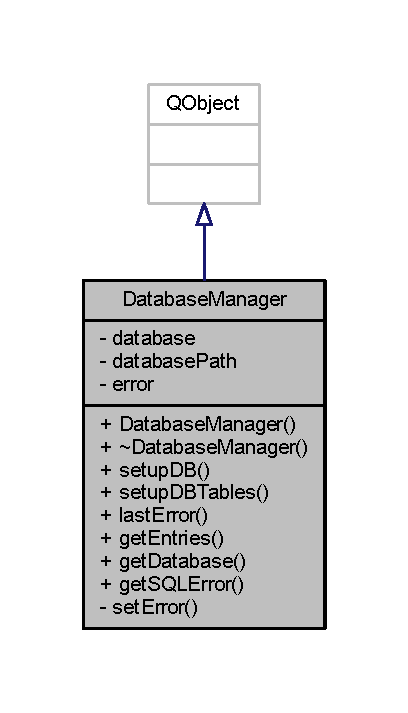
\includegraphics[width=196pt]{class_database_manager__inherit__graph}
\end{center}
\end{figure}


Collaboration diagram for Database\+Manager\+:
\nopagebreak
\begin{figure}[H]
\begin{center}
\leavevmode
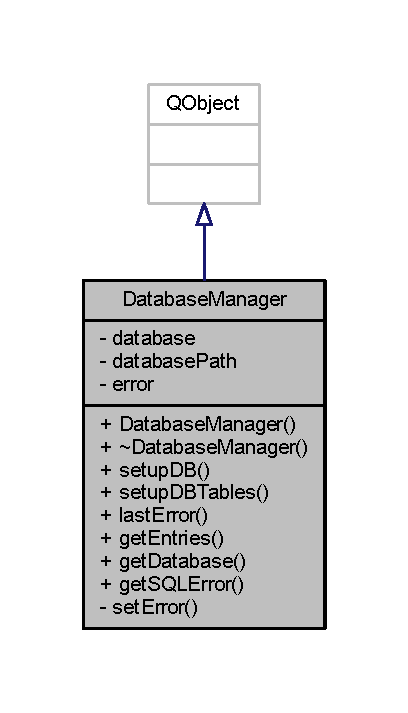
\includegraphics[width=196pt]{class_database_manager__coll__graph}
\end{center}
\end{figure}
\subsection*{Public Member Functions}
\begin{DoxyCompactItemize}
\item 
\hyperlink{class_database_manager_a957885a860c413d46e6c924c5573d89e}{Database\+Manager} (Q\+Object $\ast$parent=0)
\begin{DoxyCompactList}\small\item\em \hyperlink{class_database_manager_a957885a860c413d46e6c924c5573d89e}{Database\+Manager\+::\+Database\+Manager}. \end{DoxyCompactList}\item 
\hyperlink{class_database_manager_ae9b3a5da1e04fbb00faf8a034da1d063}{$\sim$\+Database\+Manager} ()
\begin{DoxyCompactList}\small\item\em \hyperlink{class_database_manager_ae9b3a5da1e04fbb00faf8a034da1d063}{Database\+Manager\+::$\sim$\+Database\+Manager}. \end{DoxyCompactList}\item 
bool \hyperlink{class_database_manager_a3cf904602c89c51b42ee4c66752a8989}{setup\+D\+B} ()
\begin{DoxyCompactList}\small\item\em \hyperlink{class_database_manager_a3cf904602c89c51b42ee4c66752a8989}{Database\+Manager\+::setup\+D\+B}. \end{DoxyCompactList}\item 
bool \hyperlink{class_database_manager_ad3d4a41b420d52c57a2ef4f19b031904}{setup\+D\+B\+Tables} ()
\begin{DoxyCompactList}\small\item\em \hyperlink{class_database_manager_ad3d4a41b420d52c57a2ef4f19b031904}{Database\+Manager\+::setup\+D\+B\+Tables}. \end{DoxyCompactList}\item 
Q\+Sql\+Error \hyperlink{class_database_manager_a0d786883976ea0f32e3566415138478d}{last\+Error} ()
\begin{DoxyCompactList}\small\item\em \hyperlink{class_database_manager_a0d786883976ea0f32e3566415138478d}{Database\+Manager\+::last\+Error}. \end{DoxyCompactList}\item 
Q\+Sql\+Query \hyperlink{class_database_manager_ae4cb8c8594da3342bc97a5ed325794c5}{get\+Entries} (Q\+String sql\+Statement)
\item 
Q\+Sql\+Database \hyperlink{class_database_manager_a4c1124bbf21d49013912fedac7407ce8}{get\+Database} ()
\begin{DoxyCompactList}\small\item\em \hyperlink{class_database_manager_a4c1124bbf21d49013912fedac7407ce8}{Database\+Manager\+::get\+Database}. \end{DoxyCompactList}\item 
Q\+String \hyperlink{class_database_manager_ab3c7cbe356245a5d3222147e1bb019bd}{get\+S\+Q\+L\+Error} ()
\begin{DoxyCompactList}\small\item\em \hyperlink{class_database_manager_ab3c7cbe356245a5d3222147e1bb019bd}{Database\+Manager\+::get\+S\+Q\+L\+Error}. \end{DoxyCompactList}\end{DoxyCompactItemize}
\subsection*{Private Member Functions}
\begin{DoxyCompactItemize}
\item 
void \hyperlink{class_database_manager_a0d54fec86ec216a04a38b98ef2493b9f}{set\+Error} (Q\+String alert)
\begin{DoxyCompactList}\small\item\em \hyperlink{class_database_manager_a0d54fec86ec216a04a38b98ef2493b9f}{Database\+Manager\+::set\+Error}. \end{DoxyCompactList}\end{DoxyCompactItemize}
\subsection*{Private Attributes}
\begin{DoxyCompactItemize}
\item 
Q\+Sql\+Database \hyperlink{class_database_manager_ac59e194df96c891e617fcff06a56745b}{database}
\item 
Q\+String \hyperlink{class_database_manager_ac6e7c2d8a3d5603e83c0cd36cdb4e870}{database\+Path}
\item 
Q\+String \hyperlink{class_database_manager_aeac4d1f7e240732d413d6e7d74cbaef6}{error}
\end{DoxyCompactItemize}


\subsection{Detailed Description}
The \hyperlink{class_database_manager}{Database\+Manager} class. 

\hyperlink{databasemanager_8h}{databasemanager.\+h} This manages the connection of the programm to the database.

\begin{DoxyAuthor}{Author}
Robert Wolfinger 
\end{DoxyAuthor}
\begin{DoxyVersion}{Version}
1.\+0 20.\+09.\+14 
\end{DoxyVersion}


\subsection{Constructor \& Destructor Documentation}
\hypertarget{class_database_manager_a957885a860c413d46e6c924c5573d89e}{\index{Database\+Manager@{Database\+Manager}!Database\+Manager@{Database\+Manager}}
\index{Database\+Manager@{Database\+Manager}!Database\+Manager@{Database\+Manager}}
\subsubsection[{Database\+Manager}]{\setlength{\rightskip}{0pt plus 5cm}Database\+Manager\+::\+Database\+Manager (
\begin{DoxyParamCaption}
\item[{Q\+Object $\ast$}]{parent = {\ttfamily 0}}
\end{DoxyParamCaption}
)}}\label{class_database_manager_a957885a860c413d46e6c924c5573d89e}


\hyperlink{class_database_manager_a957885a860c413d46e6c924c5573d89e}{Database\+Manager\+::\+Database\+Manager}. 

Constructs the \hyperlink{class_database_manager}{Database\+Manager} with the given parent.


\begin{DoxyParams}{Parameters}
{\em parent} & \\
\hline
\end{DoxyParams}
\hypertarget{class_database_manager_ae9b3a5da1e04fbb00faf8a034da1d063}{\index{Database\+Manager@{Database\+Manager}!````~Database\+Manager@{$\sim$\+Database\+Manager}}
\index{````~Database\+Manager@{$\sim$\+Database\+Manager}!Database\+Manager@{Database\+Manager}}
\subsubsection[{$\sim$\+Database\+Manager}]{\setlength{\rightskip}{0pt plus 5cm}Database\+Manager\+::$\sim$\+Database\+Manager (
\begin{DoxyParamCaption}
{}
\end{DoxyParamCaption}
)}}\label{class_database_manager_ae9b3a5da1e04fbb00faf8a034da1d063}


\hyperlink{class_database_manager_ae9b3a5da1e04fbb00faf8a034da1d063}{Database\+Manager\+::$\sim$\+Database\+Manager}. 

Deconstructs the \hyperlink{class_database_manager}{Database\+Manager}. All changes are being comitted and the connection is closed. 

\subsection{Member Function Documentation}
\hypertarget{class_database_manager_a4c1124bbf21d49013912fedac7407ce8}{\index{Database\+Manager@{Database\+Manager}!get\+Database@{get\+Database}}
\index{get\+Database@{get\+Database}!Database\+Manager@{Database\+Manager}}
\subsubsection[{get\+Database}]{\setlength{\rightskip}{0pt plus 5cm}Q\+Sql\+Database Database\+Manager\+::get\+Database (
\begin{DoxyParamCaption}
{}
\end{DoxyParamCaption}
)}}\label{class_database_manager_a4c1124bbf21d49013912fedac7407ce8}


\hyperlink{class_database_manager_a4c1124bbf21d49013912fedac7407ce8}{Database\+Manager\+::get\+Database}. 

Returns the database of the \hyperlink{class_database_manager}{Database\+Manager}.

\begin{DoxyReturn}{Returns}
database 
\end{DoxyReturn}
\hypertarget{class_database_manager_ae4cb8c8594da3342bc97a5ed325794c5}{\index{Database\+Manager@{Database\+Manager}!get\+Entries@{get\+Entries}}
\index{get\+Entries@{get\+Entries}!Database\+Manager@{Database\+Manager}}
\subsubsection[{get\+Entries}]{\setlength{\rightskip}{0pt plus 5cm}Q\+Sql\+Query Database\+Manager\+::get\+Entries (
\begin{DoxyParamCaption}
\item[{Q\+String}]{sql\+Statement}
\end{DoxyParamCaption}
)}}\label{class_database_manager_ae4cb8c8594da3342bc97a5ed325794c5}
\hypertarget{class_database_manager_ab3c7cbe356245a5d3222147e1bb019bd}{\index{Database\+Manager@{Database\+Manager}!get\+S\+Q\+L\+Error@{get\+S\+Q\+L\+Error}}
\index{get\+S\+Q\+L\+Error@{get\+S\+Q\+L\+Error}!Database\+Manager@{Database\+Manager}}
\subsubsection[{get\+S\+Q\+L\+Error}]{\setlength{\rightskip}{0pt plus 5cm}Q\+String Database\+Manager\+::get\+S\+Q\+L\+Error (
\begin{DoxyParamCaption}
{}
\end{DoxyParamCaption}
)}}\label{class_database_manager_ab3c7cbe356245a5d3222147e1bb019bd}


\hyperlink{class_database_manager_ab3c7cbe356245a5d3222147e1bb019bd}{Database\+Manager\+::get\+S\+Q\+L\+Error}. 

Returns the set S\+Q\+L\+Error of the \hyperlink{class_database_manager}{Database\+Manager}.

\begin{DoxyReturn}{Returns}
S\+Q\+L\+Error 
\end{DoxyReturn}
\hypertarget{class_database_manager_a0d786883976ea0f32e3566415138478d}{\index{Database\+Manager@{Database\+Manager}!last\+Error@{last\+Error}}
\index{last\+Error@{last\+Error}!Database\+Manager@{Database\+Manager}}
\subsubsection[{last\+Error}]{\setlength{\rightskip}{0pt plus 5cm}Q\+Sql\+Error Database\+Manager\+::last\+Error (
\begin{DoxyParamCaption}
{}
\end{DoxyParamCaption}
)}}\label{class_database_manager_a0d786883976ea0f32e3566415138478d}


\hyperlink{class_database_manager_a0d786883976ea0f32e3566415138478d}{Database\+Manager\+::last\+Error}. 

Returns the last error of the database.

\begin{DoxyReturn}{Returns}
Last error of the database 
\end{DoxyReturn}
\hypertarget{class_database_manager_a0d54fec86ec216a04a38b98ef2493b9f}{\index{Database\+Manager@{Database\+Manager}!set\+Error@{set\+Error}}
\index{set\+Error@{set\+Error}!Database\+Manager@{Database\+Manager}}
\subsubsection[{set\+Error}]{\setlength{\rightskip}{0pt plus 5cm}void Database\+Manager\+::set\+Error (
\begin{DoxyParamCaption}
\item[{Q\+String}]{alert}
\end{DoxyParamCaption}
)\hspace{0.3cm}{\ttfamily [private]}}}\label{class_database_manager_a0d54fec86ec216a04a38b98ef2493b9f}


\hyperlink{class_database_manager_a0d54fec86ec216a04a38b98ef2493b9f}{Database\+Manager\+::set\+Error}. 

Sets the error of the \hyperlink{class_database_manager}{Database\+Manager} from the given alert. This can be used to set for example a S\+Q\+L\+Error which is not a Database\+Error.


\begin{DoxyParams}{Parameters}
{\em alert} & \\
\hline
\end{DoxyParams}


Here is the caller graph for this function\+:
\nopagebreak
\begin{figure}[H]
\begin{center}
\leavevmode
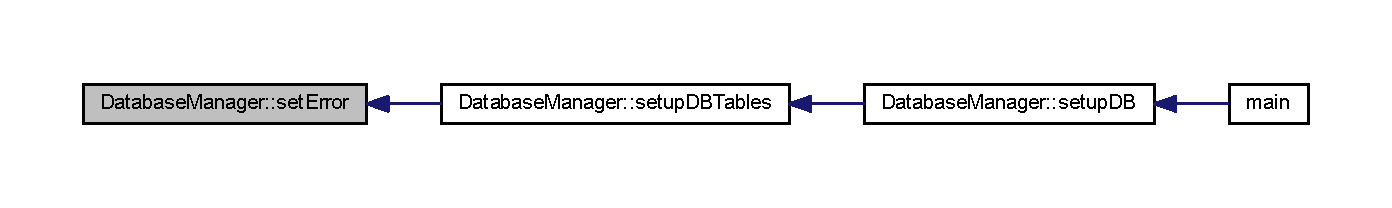
\includegraphics[width=350pt]{class_database_manager_a0d54fec86ec216a04a38b98ef2493b9f_icgraph}
\end{center}
\end{figure}


\hypertarget{class_database_manager_a3cf904602c89c51b42ee4c66752a8989}{\index{Database\+Manager@{Database\+Manager}!setup\+D\+B@{setup\+D\+B}}
\index{setup\+D\+B@{setup\+D\+B}!Database\+Manager@{Database\+Manager}}
\subsubsection[{setup\+D\+B}]{\setlength{\rightskip}{0pt plus 5cm}bool Database\+Manager\+::setup\+D\+B (
\begin{DoxyParamCaption}
{}
\end{DoxyParamCaption}
)}}\label{class_database_manager_a3cf904602c89c51b42ee4c66752a8989}


\hyperlink{class_database_manager_a3cf904602c89c51b42ee4c66752a8989}{Database\+Manager\+::setup\+D\+B}. 

Sets up the databaseconnection of the \hyperlink{class_database_manager}{Database\+Manager}.

\begin{DoxyReturn}{Returns}
success of the setup 
\end{DoxyReturn}


Here is the call graph for this function\+:
\nopagebreak
\begin{figure}[H]
\begin{center}
\leavevmode
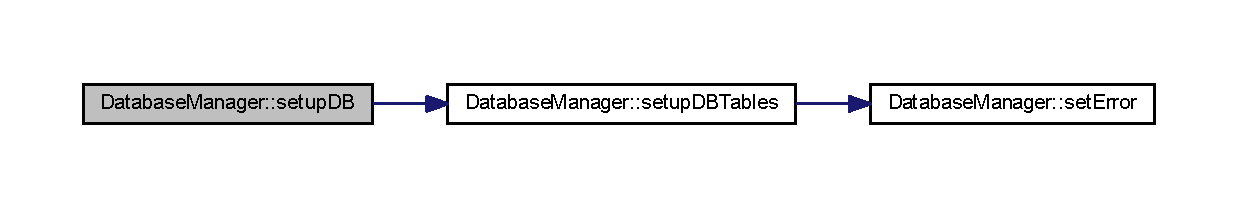
\includegraphics[width=350pt]{class_database_manager_a3cf904602c89c51b42ee4c66752a8989_cgraph}
\end{center}
\end{figure}




Here is the caller graph for this function\+:\nopagebreak
\begin{figure}[H]
\begin{center}
\leavevmode
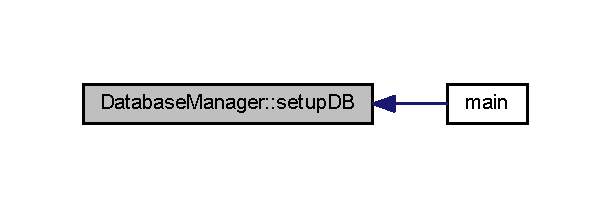
\includegraphics[width=293pt]{class_database_manager_a3cf904602c89c51b42ee4c66752a8989_icgraph}
\end{center}
\end{figure}


\hypertarget{class_database_manager_ad3d4a41b420d52c57a2ef4f19b031904}{\index{Database\+Manager@{Database\+Manager}!setup\+D\+B\+Tables@{setup\+D\+B\+Tables}}
\index{setup\+D\+B\+Tables@{setup\+D\+B\+Tables}!Database\+Manager@{Database\+Manager}}
\subsubsection[{setup\+D\+B\+Tables}]{\setlength{\rightskip}{0pt plus 5cm}bool Database\+Manager\+::setup\+D\+B\+Tables (
\begin{DoxyParamCaption}
{}
\end{DoxyParamCaption}
)}}\label{class_database_manager_ad3d4a41b420d52c57a2ef4f19b031904}


\hyperlink{class_database_manager_ad3d4a41b420d52c57a2ef4f19b031904}{Database\+Manager\+::setup\+D\+B\+Tables}. 

Creates all necessary tables in the database if they do not already exist.

\begin{DoxyReturn}{Returns}
success of setting up tables 
\end{DoxyReturn}


Here is the call graph for this function\+:
\nopagebreak
\begin{figure}[H]
\begin{center}
\leavevmode
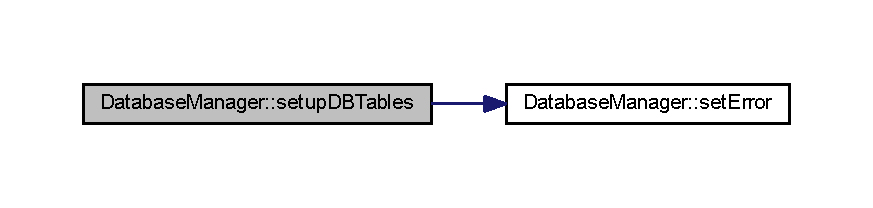
\includegraphics[width=350pt]{class_database_manager_ad3d4a41b420d52c57a2ef4f19b031904_cgraph}
\end{center}
\end{figure}




Here is the caller graph for this function\+:\nopagebreak
\begin{figure}[H]
\begin{center}
\leavevmode
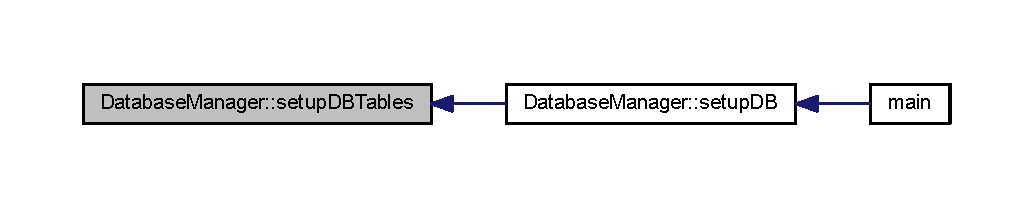
\includegraphics[width=350pt]{class_database_manager_ad3d4a41b420d52c57a2ef4f19b031904_icgraph}
\end{center}
\end{figure}




\subsection{Member Data Documentation}
\hypertarget{class_database_manager_ac59e194df96c891e617fcff06a56745b}{\index{Database\+Manager@{Database\+Manager}!database@{database}}
\index{database@{database}!Database\+Manager@{Database\+Manager}}
\subsubsection[{database}]{\setlength{\rightskip}{0pt plus 5cm}Q\+Sql\+Database Database\+Manager\+::database\hspace{0.3cm}{\ttfamily [private]}}}\label{class_database_manager_ac59e194df96c891e617fcff06a56745b}
\hypertarget{class_database_manager_ac6e7c2d8a3d5603e83c0cd36cdb4e870}{\index{Database\+Manager@{Database\+Manager}!database\+Path@{database\+Path}}
\index{database\+Path@{database\+Path}!Database\+Manager@{Database\+Manager}}
\subsubsection[{database\+Path}]{\setlength{\rightskip}{0pt plus 5cm}Q\+String Database\+Manager\+::database\+Path\hspace{0.3cm}{\ttfamily [private]}}}\label{class_database_manager_ac6e7c2d8a3d5603e83c0cd36cdb4e870}
\hypertarget{class_database_manager_aeac4d1f7e240732d413d6e7d74cbaef6}{\index{Database\+Manager@{Database\+Manager}!error@{error}}
\index{error@{error}!Database\+Manager@{Database\+Manager}}
\subsubsection[{error}]{\setlength{\rightskip}{0pt plus 5cm}Q\+String Database\+Manager\+::error\hspace{0.3cm}{\ttfamily [private]}}}\label{class_database_manager_aeac4d1f7e240732d413d6e7d74cbaef6}


The documentation for this class was generated from the following files\+:\begin{DoxyCompactItemize}
\item 
D\+:/\+Entwicklung/\+C++/\+Workspace/\+Beleg\+Cpp/\hyperlink{databasemanager_8h}{databasemanager.\+h}\item 
D\+:/\+Entwicklung/\+C++/\+Workspace/\+Beleg\+Cpp/\hyperlink{databasemanager_8cpp}{databasemanager.\+cpp}\end{DoxyCompactItemize}

\hypertarget{class_dialog_help}{\section{Dialog\+Help Class Reference}
\label{class_dialog_help}\index{Dialog\+Help@{Dialog\+Help}}
}


The \hyperlink{class_dialog_help}{Dialog\+Help} class.  




{\ttfamily \#include $<$dialoghelp.\+h$>$}



Inheritance diagram for Dialog\+Help\+:
\nopagebreak
\begin{figure}[H]
\begin{center}
\leavevmode
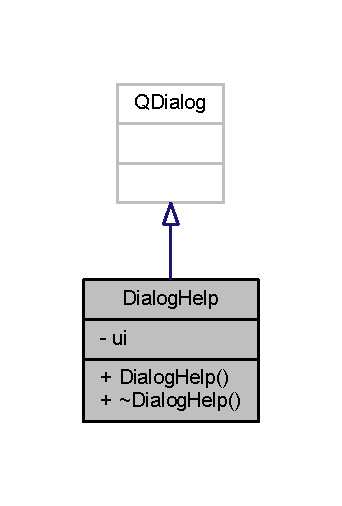
\includegraphics[width=164pt]{class_dialog_help__inherit__graph}
\end{center}
\end{figure}


Collaboration diagram for Dialog\+Help\+:
\nopagebreak
\begin{figure}[H]
\begin{center}
\leavevmode
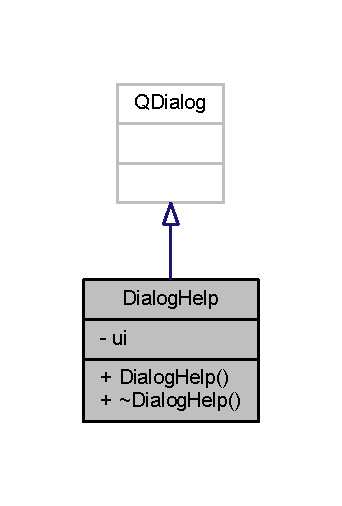
\includegraphics[width=164pt]{class_dialog_help__coll__graph}
\end{center}
\end{figure}
\subsection*{Public Member Functions}
\begin{DoxyCompactItemize}
\item 
\hyperlink{class_dialog_help_a8c9e470d3a7a8b2e28c4e59d020bf51e}{Dialog\+Help} (Q\+Widget $\ast$parent=0)
\begin{DoxyCompactList}\small\item\em \hyperlink{class_dialog_help_a8c9e470d3a7a8b2e28c4e59d020bf51e}{Dialog\+Help\+::\+Dialog\+Help}. \end{DoxyCompactList}\item 
\hyperlink{class_dialog_help_a4c076a8c67ad264caf067c9135911839}{$\sim$\+Dialog\+Help} ()
\begin{DoxyCompactList}\small\item\em \hyperlink{class_dialog_help_a4c076a8c67ad264caf067c9135911839}{Dialog\+Help\+::$\sim$\+Dialog\+Help}. \end{DoxyCompactList}\end{DoxyCompactItemize}
\subsection*{Private Attributes}
\begin{DoxyCompactItemize}
\item 
Ui\+::\+Dialog\+Help $\ast$ \hyperlink{class_dialog_help_a7e241423eb5ac274a3f1bde98ad625dd}{ui}
\end{DoxyCompactItemize}


\subsection{Detailed Description}
The \hyperlink{class_dialog_help}{Dialog\+Help} class. 

This class represents the Helpdialog.

\begin{DoxyAuthor}{Author}
Robert Wolfinger 
\end{DoxyAuthor}
\begin{DoxyVersion}{Version}
1.\+0 20.\+09.\+14 
\end{DoxyVersion}


\subsection{Constructor \& Destructor Documentation}
\hypertarget{class_dialog_help_a8c9e470d3a7a8b2e28c4e59d020bf51e}{\index{Dialog\+Help@{Dialog\+Help}!Dialog\+Help@{Dialog\+Help}}
\index{Dialog\+Help@{Dialog\+Help}!Dialog\+Help@{Dialog\+Help}}
\subsubsection[{Dialog\+Help}]{\setlength{\rightskip}{0pt plus 5cm}Dialog\+Help\+::\+Dialog\+Help (
\begin{DoxyParamCaption}
\item[{Q\+Widget $\ast$}]{parent = {\ttfamily 0}}
\end{DoxyParamCaption}
)\hspace{0.3cm}{\ttfamily [explicit]}}}\label{class_dialog_help_a8c9e470d3a7a8b2e28c4e59d020bf51e}


\hyperlink{class_dialog_help_a8c9e470d3a7a8b2e28c4e59d020bf51e}{Dialog\+Help\+::\+Dialog\+Help}. 

\begin{DoxyAuthor}{Author}
Robert Wolfinger 
\end{DoxyAuthor}
\begin{DoxyVersion}{Version}
1.\+0 20.\+09.\+14 Constructs the \hyperlink{class_dialog_help}{Dialog\+Help} the given parent. Sets up the Dialog and reads the readme.\+html file into the textbrowser.
\end{DoxyVersion}

\begin{DoxyParams}{Parameters}
{\em parent} & \\
\hline
\end{DoxyParams}
\hypertarget{class_dialog_help_a4c076a8c67ad264caf067c9135911839}{\index{Dialog\+Help@{Dialog\+Help}!````~Dialog\+Help@{$\sim$\+Dialog\+Help}}
\index{````~Dialog\+Help@{$\sim$\+Dialog\+Help}!Dialog\+Help@{Dialog\+Help}}
\subsubsection[{$\sim$\+Dialog\+Help}]{\setlength{\rightskip}{0pt plus 5cm}Dialog\+Help\+::$\sim$\+Dialog\+Help (
\begin{DoxyParamCaption}
{}
\end{DoxyParamCaption}
)}}\label{class_dialog_help_a4c076a8c67ad264caf067c9135911839}


\hyperlink{class_dialog_help_a4c076a8c67ad264caf067c9135911839}{Dialog\+Help\+::$\sim$\+Dialog\+Help}. 

Deconstructs the Dialog. 

\subsection{Member Data Documentation}
\hypertarget{class_dialog_help_a7e241423eb5ac274a3f1bde98ad625dd}{\index{Dialog\+Help@{Dialog\+Help}!ui@{ui}}
\index{ui@{ui}!Dialog\+Help@{Dialog\+Help}}
\subsubsection[{ui}]{\setlength{\rightskip}{0pt plus 5cm}Ui\+::\+Dialog\+Help$\ast$ Dialog\+Help\+::ui\hspace{0.3cm}{\ttfamily [private]}}}\label{class_dialog_help_a7e241423eb5ac274a3f1bde98ad625dd}


The documentation for this class was generated from the following files\+:\begin{DoxyCompactItemize}
\item 
D\+:/\+Entwicklung/\+C++/\+Workspace/\+Beleg\+Cpp/\hyperlink{dialoghelp_8h}{dialoghelp.\+h}\item 
D\+:/\+Entwicklung/\+C++/\+Workspace/\+Beleg\+Cpp/\hyperlink{dialoghelp_8cpp}{dialoghelp.\+cpp}\end{DoxyCompactItemize}

\hypertarget{class_dialog_new_entry}{\section{Dialog\+New\+Entry Class Reference}
\label{class_dialog_new_entry}\index{Dialog\+New\+Entry@{Dialog\+New\+Entry}}
}


The \hyperlink{class_dialog_new_entry}{Dialog\+New\+Entry} class.  




{\ttfamily \#include $<$dialognewentry.\+h$>$}



Inheritance diagram for Dialog\+New\+Entry\+:
\nopagebreak
\begin{figure}[H]
\begin{center}
\leavevmode
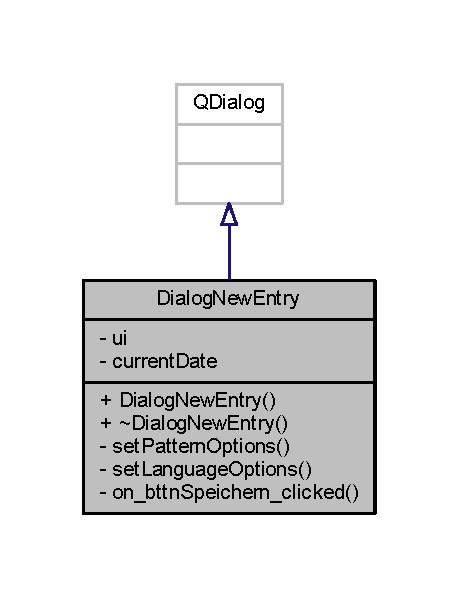
\includegraphics[width=220pt]{class_dialog_new_entry__inherit__graph}
\end{center}
\end{figure}


Collaboration diagram for Dialog\+New\+Entry\+:
\nopagebreak
\begin{figure}[H]
\begin{center}
\leavevmode
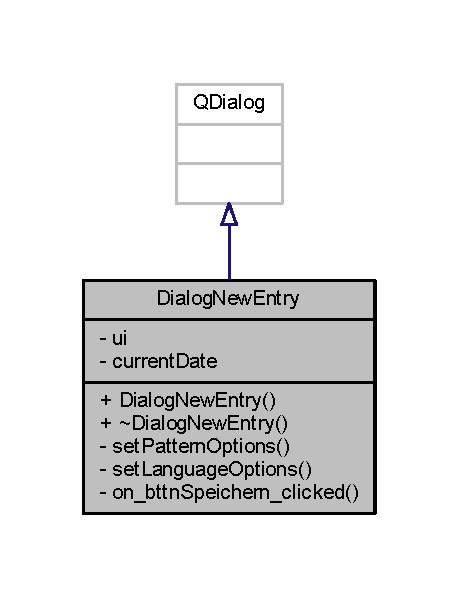
\includegraphics[width=220pt]{class_dialog_new_entry__coll__graph}
\end{center}
\end{figure}
\subsection*{Public Member Functions}
\begin{DoxyCompactItemize}
\item 
\hyperlink{class_dialog_new_entry_adf5d314059f2ddb1d49035df63279b47}{Dialog\+New\+Entry} (Q\+Widget $\ast$parent=0)
\begin{DoxyCompactList}\small\item\em \hyperlink{class_dialog_new_entry_adf5d314059f2ddb1d49035df63279b47}{Dialog\+New\+Entry\+::\+Dialog\+New\+Entry}. \end{DoxyCompactList}\item 
\hyperlink{class_dialog_new_entry_aea9c132ba82fba5dc62a017257be0e89}{$\sim$\+Dialog\+New\+Entry} ()
\begin{DoxyCompactList}\small\item\em \hyperlink{class_dialog_new_entry_aea9c132ba82fba5dc62a017257be0e89}{Dialog\+New\+Entry\+::$\sim$\+Dialog\+New\+Entry}. \end{DoxyCompactList}\end{DoxyCompactItemize}
\subsection*{Private Slots}
\begin{DoxyCompactItemize}
\item 
void \hyperlink{class_dialog_new_entry_a3ca9da6355dbe206ea01975d2b37e72a}{on\+\_\+bttn\+Speichern\+\_\+clicked} ()
\begin{DoxyCompactList}\small\item\em \hyperlink{class_dialog_new_entry_a3ca9da6355dbe206ea01975d2b37e72a}{Dialog\+New\+Entry\+::on\+\_\+bttn\+Speichern\+\_\+clicked}. \end{DoxyCompactList}\end{DoxyCompactItemize}
\subsection*{Private Member Functions}
\begin{DoxyCompactItemize}
\item 
void \hyperlink{class_dialog_new_entry_a419783c0f14219c207dcd5946fc302a2}{set\+Pattern\+Options} ()
\begin{DoxyCompactList}\small\item\em \hyperlink{class_dialog_new_entry_a419783c0f14219c207dcd5946fc302a2}{Dialog\+New\+Entry\+::set\+Pattern\+Options}. \end{DoxyCompactList}\item 
void \hyperlink{class_dialog_new_entry_a23ba49e12a08f09848d5d72a772e5a0e}{set\+Language\+Options} ()
\begin{DoxyCompactList}\small\item\em \hyperlink{class_dialog_new_entry_a23ba49e12a08f09848d5d72a772e5a0e}{Dialog\+New\+Entry\+::set\+Language\+Options}. \end{DoxyCompactList}\end{DoxyCompactItemize}
\subsection*{Private Attributes}
\begin{DoxyCompactItemize}
\item 
Ui\+::\+Dialog\+New\+Entry $\ast$ \hyperlink{class_dialog_new_entry_a793dbaf0032320cdc11a683fe27c30f0}{ui}
\item 
Q\+Date \hyperlink{class_dialog_new_entry_a2caaaa17bdf2e1ce91cf21a162d32c03}{current\+Date}
\end{DoxyCompactItemize}


\subsection{Detailed Description}
The \hyperlink{class_dialog_new_entry}{Dialog\+New\+Entry} class. 

This class represents the Q\+Dialog for creating a new entry.

\begin{DoxyAuthor}{Author}
Robert Wolfinger 
\end{DoxyAuthor}
\begin{DoxyVersion}{Version}
1.\+0 20.\+09.\+14 
\end{DoxyVersion}


\subsection{Constructor \& Destructor Documentation}
\hypertarget{class_dialog_new_entry_adf5d314059f2ddb1d49035df63279b47}{\index{Dialog\+New\+Entry@{Dialog\+New\+Entry}!Dialog\+New\+Entry@{Dialog\+New\+Entry}}
\index{Dialog\+New\+Entry@{Dialog\+New\+Entry}!Dialog\+New\+Entry@{Dialog\+New\+Entry}}
\subsubsection[{Dialog\+New\+Entry}]{\setlength{\rightskip}{0pt plus 5cm}Dialog\+New\+Entry\+::\+Dialog\+New\+Entry (
\begin{DoxyParamCaption}
\item[{Q\+Widget $\ast$}]{parent = {\ttfamily 0}}
\end{DoxyParamCaption}
)\hspace{0.3cm}{\ttfamily [explicit]}}}\label{class_dialog_new_entry_adf5d314059f2ddb1d49035df63279b47}


\hyperlink{class_dialog_new_entry_adf5d314059f2ddb1d49035df63279b47}{Dialog\+New\+Entry\+::\+Dialog\+New\+Entry}. 

\begin{DoxyAuthor}{Author}
Robert Wolfinger 
\end{DoxyAuthor}
\begin{DoxyVersion}{Version}
1.\+0 20.\+09.\+14 Constructs the Dialog with the given parent. Sets up the Date and Language/\+Pattern-\/\+Options
\end{DoxyVersion}

\begin{DoxyParams}{Parameters}
{\em parent} & \\
\hline
\end{DoxyParams}


Here is the call graph for this function\+:
\nopagebreak
\begin{figure}[H]
\begin{center}
\leavevmode
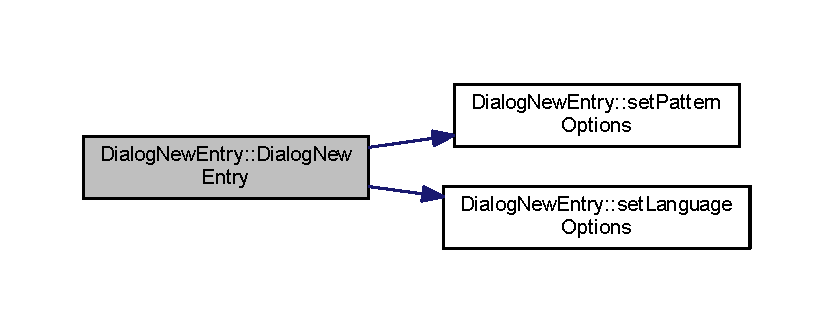
\includegraphics[width=350pt]{class_dialog_new_entry_adf5d314059f2ddb1d49035df63279b47_cgraph}
\end{center}
\end{figure}


\hypertarget{class_dialog_new_entry_aea9c132ba82fba5dc62a017257be0e89}{\index{Dialog\+New\+Entry@{Dialog\+New\+Entry}!````~Dialog\+New\+Entry@{$\sim$\+Dialog\+New\+Entry}}
\index{````~Dialog\+New\+Entry@{$\sim$\+Dialog\+New\+Entry}!Dialog\+New\+Entry@{Dialog\+New\+Entry}}
\subsubsection[{$\sim$\+Dialog\+New\+Entry}]{\setlength{\rightskip}{0pt plus 5cm}Dialog\+New\+Entry\+::$\sim$\+Dialog\+New\+Entry (
\begin{DoxyParamCaption}
{}
\end{DoxyParamCaption}
)}}\label{class_dialog_new_entry_aea9c132ba82fba5dc62a017257be0e89}


\hyperlink{class_dialog_new_entry_aea9c132ba82fba5dc62a017257be0e89}{Dialog\+New\+Entry\+::$\sim$\+Dialog\+New\+Entry}. 

Deconstructs the Dialog 

\subsection{Member Function Documentation}
\hypertarget{class_dialog_new_entry_a3ca9da6355dbe206ea01975d2b37e72a}{\index{Dialog\+New\+Entry@{Dialog\+New\+Entry}!on\+\_\+bttn\+Speichern\+\_\+clicked@{on\+\_\+bttn\+Speichern\+\_\+clicked}}
\index{on\+\_\+bttn\+Speichern\+\_\+clicked@{on\+\_\+bttn\+Speichern\+\_\+clicked}!Dialog\+New\+Entry@{Dialog\+New\+Entry}}
\subsubsection[{on\+\_\+bttn\+Speichern\+\_\+clicked}]{\setlength{\rightskip}{0pt plus 5cm}void Dialog\+New\+Entry\+::on\+\_\+bttn\+Speichern\+\_\+clicked (
\begin{DoxyParamCaption}
{}
\end{DoxyParamCaption}
)\hspace{0.3cm}{\ttfamily [private]}, {\ttfamily [slot]}}}\label{class_dialog_new_entry_a3ca9da6355dbe206ea01975d2b37e72a}


\hyperlink{class_dialog_new_entry_a3ca9da6355dbe206ea01975d2b37e72a}{Dialog\+New\+Entry\+::on\+\_\+bttn\+Speichern\+\_\+clicked}. 

Saves all filled fields as an entry to the database \hypertarget{class_dialog_new_entry_a23ba49e12a08f09848d5d72a772e5a0e}{\index{Dialog\+New\+Entry@{Dialog\+New\+Entry}!set\+Language\+Options@{set\+Language\+Options}}
\index{set\+Language\+Options@{set\+Language\+Options}!Dialog\+New\+Entry@{Dialog\+New\+Entry}}
\subsubsection[{set\+Language\+Options}]{\setlength{\rightskip}{0pt plus 5cm}void Dialog\+New\+Entry\+::set\+Language\+Options (
\begin{DoxyParamCaption}
{}
\end{DoxyParamCaption}
)\hspace{0.3cm}{\ttfamily [private]}}}\label{class_dialog_new_entry_a23ba49e12a08f09848d5d72a772e5a0e}


\hyperlink{class_dialog_new_entry_a23ba49e12a08f09848d5d72a772e5a0e}{Dialog\+New\+Entry\+::set\+Language\+Options}. 

Retrieves all languages from the database and adds them to the options. 

Here is the caller graph for this function\+:
\nopagebreak
\begin{figure}[H]
\begin{center}
\leavevmode
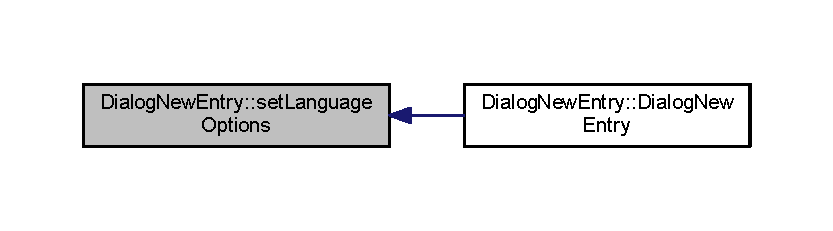
\includegraphics[width=350pt]{class_dialog_new_entry_a23ba49e12a08f09848d5d72a772e5a0e_icgraph}
\end{center}
\end{figure}


\hypertarget{class_dialog_new_entry_a419783c0f14219c207dcd5946fc302a2}{\index{Dialog\+New\+Entry@{Dialog\+New\+Entry}!set\+Pattern\+Options@{set\+Pattern\+Options}}
\index{set\+Pattern\+Options@{set\+Pattern\+Options}!Dialog\+New\+Entry@{Dialog\+New\+Entry}}
\subsubsection[{set\+Pattern\+Options}]{\setlength{\rightskip}{0pt plus 5cm}void Dialog\+New\+Entry\+::set\+Pattern\+Options (
\begin{DoxyParamCaption}
{}
\end{DoxyParamCaption}
)\hspace{0.3cm}{\ttfamily [private]}}}\label{class_dialog_new_entry_a419783c0f14219c207dcd5946fc302a2}


\hyperlink{class_dialog_new_entry_a419783c0f14219c207dcd5946fc302a2}{Dialog\+New\+Entry\+::set\+Pattern\+Options}. 

Retrieves all patterns from the database and adds them to the options. 

Here is the caller graph for this function\+:
\nopagebreak
\begin{figure}[H]
\begin{center}
\leavevmode
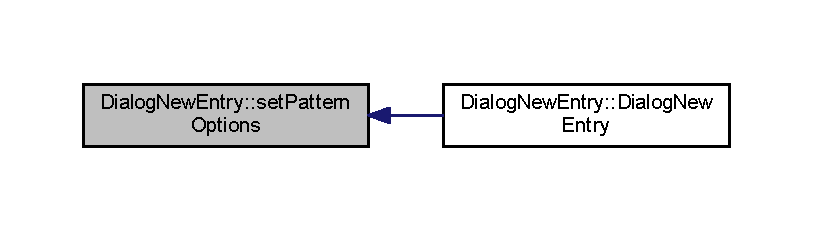
\includegraphics[width=350pt]{class_dialog_new_entry_a419783c0f14219c207dcd5946fc302a2_icgraph}
\end{center}
\end{figure}




\subsection{Member Data Documentation}
\hypertarget{class_dialog_new_entry_a2caaaa17bdf2e1ce91cf21a162d32c03}{\index{Dialog\+New\+Entry@{Dialog\+New\+Entry}!current\+Date@{current\+Date}}
\index{current\+Date@{current\+Date}!Dialog\+New\+Entry@{Dialog\+New\+Entry}}
\subsubsection[{current\+Date}]{\setlength{\rightskip}{0pt plus 5cm}Q\+Date Dialog\+New\+Entry\+::current\+Date\hspace{0.3cm}{\ttfamily [private]}}}\label{class_dialog_new_entry_a2caaaa17bdf2e1ce91cf21a162d32c03}
\hypertarget{class_dialog_new_entry_a793dbaf0032320cdc11a683fe27c30f0}{\index{Dialog\+New\+Entry@{Dialog\+New\+Entry}!ui@{ui}}
\index{ui@{ui}!Dialog\+New\+Entry@{Dialog\+New\+Entry}}
\subsubsection[{ui}]{\setlength{\rightskip}{0pt plus 5cm}Ui\+::\+Dialog\+New\+Entry$\ast$ Dialog\+New\+Entry\+::ui\hspace{0.3cm}{\ttfamily [private]}}}\label{class_dialog_new_entry_a793dbaf0032320cdc11a683fe27c30f0}


The documentation for this class was generated from the following files\+:\begin{DoxyCompactItemize}
\item 
D\+:/\+Entwicklung/\+C++/\+Workspace/\+Beleg\+Cpp/\hyperlink{dialognewentry_8h}{dialognewentry.\+h}\item 
D\+:/\+Entwicklung/\+C++/\+Workspace/\+Beleg\+Cpp/\hyperlink{dialognewentry_8cpp}{dialognewentry.\+cpp}\end{DoxyCompactItemize}

\hypertarget{class_dialog_search_criteria}{\section{Dialog\+Search\+Criteria Class Reference}
\label{class_dialog_search_criteria}\index{Dialog\+Search\+Criteria@{Dialog\+Search\+Criteria}}
}


The \hyperlink{class_dialog_search_criteria}{Dialog\+Search\+Criteria} class.  




{\ttfamily \#include $<$dialogsearchcriteria.\+h$>$}



Inheritance diagram for Dialog\+Search\+Criteria\+:
\nopagebreak
\begin{figure}[H]
\begin{center}
\leavevmode
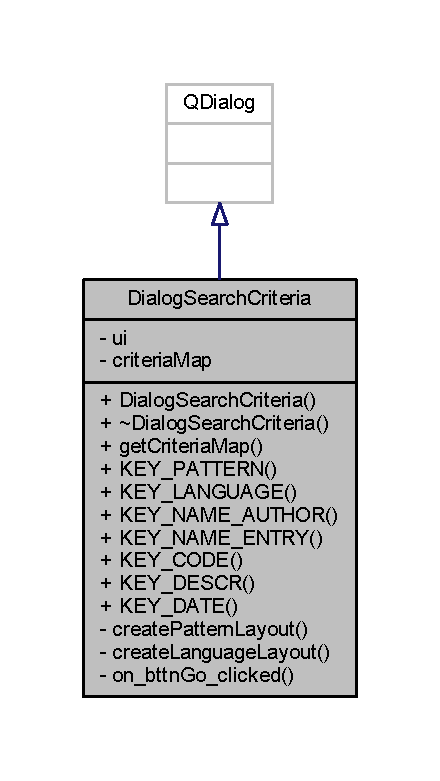
\includegraphics[width=211pt]{class_dialog_search_criteria__inherit__graph}
\end{center}
\end{figure}


Collaboration diagram for Dialog\+Search\+Criteria\+:
\nopagebreak
\begin{figure}[H]
\begin{center}
\leavevmode
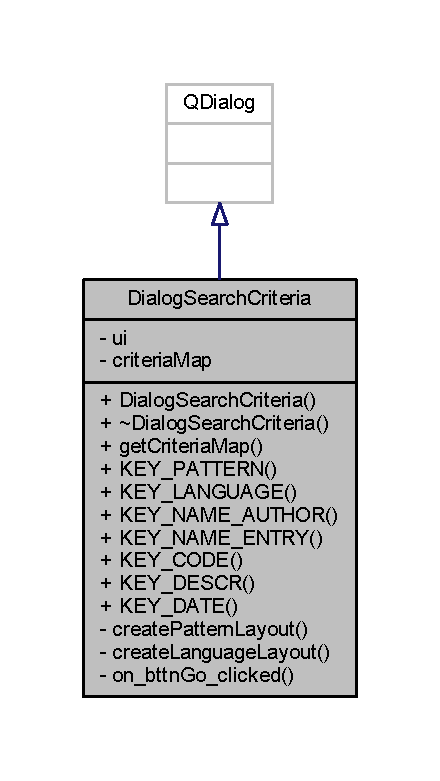
\includegraphics[width=211pt]{class_dialog_search_criteria__coll__graph}
\end{center}
\end{figure}
\subsection*{Public Member Functions}
\begin{DoxyCompactItemize}
\item 
\hyperlink{class_dialog_search_criteria_a1f739719a87720517a8c1c8034ab4f83}{Dialog\+Search\+Criteria} (Q\+Widget $\ast$parent=0)
\begin{DoxyCompactList}\small\item\em \hyperlink{class_dialog_search_criteria_a1f739719a87720517a8c1c8034ab4f83}{Dialog\+Search\+Criteria\+::\+Dialog\+Search\+Criteria}. \end{DoxyCompactList}\item 
\hyperlink{class_dialog_search_criteria_af48ae5e81e28ddcc2a209f3d2e5a10fd}{$\sim$\+Dialog\+Search\+Criteria} ()
\begin{DoxyCompactList}\small\item\em \hyperlink{class_dialog_search_criteria_af48ae5e81e28ddcc2a209f3d2e5a10fd}{Dialog\+Search\+Criteria\+::$\sim$\+Dialog\+Search\+Criteria}. \end{DoxyCompactList}\item 
Q\+Multi\+Map$<$ Q\+String, Q\+String $>$ \hyperlink{class_dialog_search_criteria_a4580f445b0386b977d30694afd0d0c22}{get\+Criteria\+Map} ()
\begin{DoxyCompactList}\small\item\em \hyperlink{class_dialog_search_criteria_a4580f445b0386b977d30694afd0d0c22}{Dialog\+Search\+Criteria\+::get\+Criteria\+Map}. \end{DoxyCompactList}\end{DoxyCompactItemize}
\subsection*{Static Public Member Functions}
\begin{DoxyCompactItemize}
\item 
static const Q\+String \hyperlink{class_dialog_search_criteria_a855feb356d17d2631bf7251f1a501ce1}{K\+E\+Y\+\_\+\+P\+A\+T\+T\+E\+R\+N} ()
\item 
static const Q\+String \hyperlink{class_dialog_search_criteria_a3f9f43120bea93348999826e4071310d}{K\+E\+Y\+\_\+\+L\+A\+N\+G\+U\+A\+G\+E} ()
\item 
static const Q\+String \hyperlink{class_dialog_search_criteria_ac49318706a518f848fe9b4902c120e8d}{K\+E\+Y\+\_\+\+N\+A\+M\+E\+\_\+\+A\+U\+T\+H\+O\+R} ()
\item 
static const Q\+String \hyperlink{class_dialog_search_criteria_a9b57352b785dc4b716e171c7835b0ff8}{K\+E\+Y\+\_\+\+N\+A\+M\+E\+\_\+\+E\+N\+T\+R\+Y} ()
\item 
static const Q\+String \hyperlink{class_dialog_search_criteria_a874909d0b8c007695ef40120bc290157}{K\+E\+Y\+\_\+\+C\+O\+D\+E} ()
\item 
static const Q\+String \hyperlink{class_dialog_search_criteria_a8c29bb9a9d48246950ff23abee75d059}{K\+E\+Y\+\_\+\+D\+E\+S\+C\+R} ()
\item 
static const Q\+String \hyperlink{class_dialog_search_criteria_a2db45b1bebeb55547c213dd558342bb7}{K\+E\+Y\+\_\+\+D\+A\+T\+E} ()
\end{DoxyCompactItemize}
\subsection*{Private Slots}
\begin{DoxyCompactItemize}
\item 
void \hyperlink{class_dialog_search_criteria_a0e106dc53e15508c8d8bf59308870371}{on\+\_\+bttn\+Go\+\_\+clicked} ()
\begin{DoxyCompactList}\small\item\em \hyperlink{class_dialog_search_criteria_a0e106dc53e15508c8d8bf59308870371}{Dialog\+Search\+Criteria\+::on\+\_\+bttn\+Go\+\_\+clicked}. \end{DoxyCompactList}\end{DoxyCompactItemize}
\subsection*{Private Member Functions}
\begin{DoxyCompactItemize}
\item 
void \hyperlink{class_dialog_search_criteria_a0b4af6adf36d8fc7a4e6c7b29743e777}{create\+Pattern\+Layout} ()
\begin{DoxyCompactList}\small\item\em \hyperlink{class_dialog_search_criteria_a0b4af6adf36d8fc7a4e6c7b29743e777}{Dialog\+Search\+Criteria\+::create\+Pattern\+Layout}. \end{DoxyCompactList}\item 
void \hyperlink{class_dialog_search_criteria_adf3d7d1a2c6067edcb828f842cdb72ff}{create\+Language\+Layout} ()
\begin{DoxyCompactList}\small\item\em \hyperlink{class_dialog_search_criteria_adf3d7d1a2c6067edcb828f842cdb72ff}{Dialog\+Search\+Criteria\+::create\+Language\+Layout}. \end{DoxyCompactList}\end{DoxyCompactItemize}
\subsection*{Private Attributes}
\begin{DoxyCompactItemize}
\item 
Ui\+::\+Dialog\+Search\+Criteria $\ast$ \hyperlink{class_dialog_search_criteria_a7e7d05c4b1937aec851d514e19182c50}{ui}
\item 
Q\+Multi\+Map$<$ Q\+String, Q\+String $>$ \hyperlink{class_dialog_search_criteria_a3ed8b9ec17d79f4e995926e2ba7e02b4}{criteria\+Map}
\end{DoxyCompactItemize}


\subsection{Detailed Description}
The \hyperlink{class_dialog_search_criteria}{Dialog\+Search\+Criteria} class. 

This class represents the Q\+Dialog to set the search criteria.

\begin{DoxyAuthor}{Author}
Robert Wolfinger 
\end{DoxyAuthor}
\begin{DoxyVersion}{Version}
1.\+0 20.\+09.\+14 
\end{DoxyVersion}


\subsection{Constructor \& Destructor Documentation}
\hypertarget{class_dialog_search_criteria_a1f739719a87720517a8c1c8034ab4f83}{\index{Dialog\+Search\+Criteria@{Dialog\+Search\+Criteria}!Dialog\+Search\+Criteria@{Dialog\+Search\+Criteria}}
\index{Dialog\+Search\+Criteria@{Dialog\+Search\+Criteria}!Dialog\+Search\+Criteria@{Dialog\+Search\+Criteria}}
\subsubsection[{Dialog\+Search\+Criteria}]{\setlength{\rightskip}{0pt plus 5cm}Dialog\+Search\+Criteria\+::\+Dialog\+Search\+Criteria (
\begin{DoxyParamCaption}
\item[{Q\+Widget $\ast$}]{parent = {\ttfamily 0}}
\end{DoxyParamCaption}
)\hspace{0.3cm}{\ttfamily [explicit]}}}\label{class_dialog_search_criteria_a1f739719a87720517a8c1c8034ab4f83}


\hyperlink{class_dialog_search_criteria_a1f739719a87720517a8c1c8034ab4f83}{Dialog\+Search\+Criteria\+::\+Dialog\+Search\+Criteria}. 

\begin{DoxyAuthor}{Author}
Robert Wolfinger 
\end{DoxyAuthor}
\begin{DoxyVersion}{Version}
1.\+0 20.\+09.\+14 Constructs the dialog. Sets up patterns, languages and the date.
\end{DoxyVersion}

\begin{DoxyParams}{Parameters}
{\em parent} & \\
\hline
\end{DoxyParams}


Here is the call graph for this function\+:
\nopagebreak
\begin{figure}[H]
\begin{center}
\leavevmode
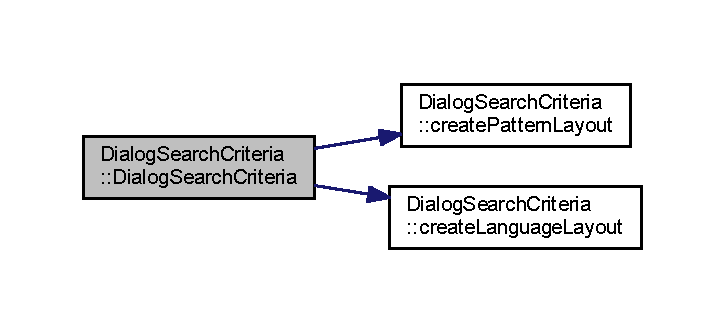
\includegraphics[width=348pt]{class_dialog_search_criteria_a1f739719a87720517a8c1c8034ab4f83_cgraph}
\end{center}
\end{figure}


\hypertarget{class_dialog_search_criteria_af48ae5e81e28ddcc2a209f3d2e5a10fd}{\index{Dialog\+Search\+Criteria@{Dialog\+Search\+Criteria}!````~Dialog\+Search\+Criteria@{$\sim$\+Dialog\+Search\+Criteria}}
\index{````~Dialog\+Search\+Criteria@{$\sim$\+Dialog\+Search\+Criteria}!Dialog\+Search\+Criteria@{Dialog\+Search\+Criteria}}
\subsubsection[{$\sim$\+Dialog\+Search\+Criteria}]{\setlength{\rightskip}{0pt plus 5cm}Dialog\+Search\+Criteria\+::$\sim$\+Dialog\+Search\+Criteria (
\begin{DoxyParamCaption}
{}
\end{DoxyParamCaption}
)}}\label{class_dialog_search_criteria_af48ae5e81e28ddcc2a209f3d2e5a10fd}


\hyperlink{class_dialog_search_criteria_af48ae5e81e28ddcc2a209f3d2e5a10fd}{Dialog\+Search\+Criteria\+::$\sim$\+Dialog\+Search\+Criteria}. 

Deconstructs the dialog. 

\subsection{Member Function Documentation}
\hypertarget{class_dialog_search_criteria_adf3d7d1a2c6067edcb828f842cdb72ff}{\index{Dialog\+Search\+Criteria@{Dialog\+Search\+Criteria}!create\+Language\+Layout@{create\+Language\+Layout}}
\index{create\+Language\+Layout@{create\+Language\+Layout}!Dialog\+Search\+Criteria@{Dialog\+Search\+Criteria}}
\subsubsection[{create\+Language\+Layout}]{\setlength{\rightskip}{0pt plus 5cm}void Dialog\+Search\+Criteria\+::create\+Language\+Layout (
\begin{DoxyParamCaption}
{}
\end{DoxyParamCaption}
)\hspace{0.3cm}{\ttfamily [private]}}}\label{class_dialog_search_criteria_adf3d7d1a2c6067edcb828f842cdb72ff}


\hyperlink{class_dialog_search_criteria_adf3d7d1a2c6067edcb828f842cdb72ff}{Dialog\+Search\+Criteria\+::create\+Language\+Layout}. 

Creates the layout for the languages after retrieving them from the database. 

Here is the caller graph for this function\+:
\nopagebreak
\begin{figure}[H]
\begin{center}
\leavevmode
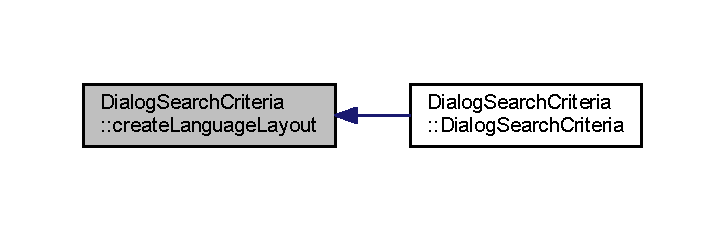
\includegraphics[width=348pt]{class_dialog_search_criteria_adf3d7d1a2c6067edcb828f842cdb72ff_icgraph}
\end{center}
\end{figure}


\hypertarget{class_dialog_search_criteria_a0b4af6adf36d8fc7a4e6c7b29743e777}{\index{Dialog\+Search\+Criteria@{Dialog\+Search\+Criteria}!create\+Pattern\+Layout@{create\+Pattern\+Layout}}
\index{create\+Pattern\+Layout@{create\+Pattern\+Layout}!Dialog\+Search\+Criteria@{Dialog\+Search\+Criteria}}
\subsubsection[{create\+Pattern\+Layout}]{\setlength{\rightskip}{0pt plus 5cm}void Dialog\+Search\+Criteria\+::create\+Pattern\+Layout (
\begin{DoxyParamCaption}
{}
\end{DoxyParamCaption}
)\hspace{0.3cm}{\ttfamily [private]}}}\label{class_dialog_search_criteria_a0b4af6adf36d8fc7a4e6c7b29743e777}


\hyperlink{class_dialog_search_criteria_a0b4af6adf36d8fc7a4e6c7b29743e777}{Dialog\+Search\+Criteria\+::create\+Pattern\+Layout}. 

Creates the layout for the patterns after retrieving them from the database. 

Here is the caller graph for this function\+:
\nopagebreak
\begin{figure}[H]
\begin{center}
\leavevmode
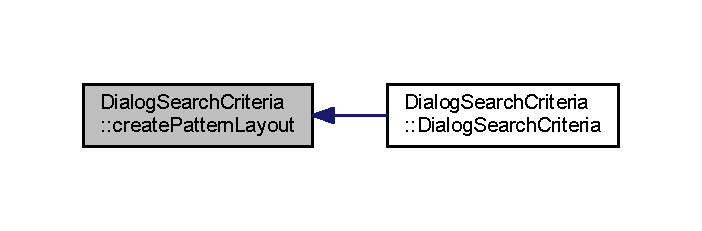
\includegraphics[width=337pt]{class_dialog_search_criteria_a0b4af6adf36d8fc7a4e6c7b29743e777_icgraph}
\end{center}
\end{figure}


\hypertarget{class_dialog_search_criteria_a4580f445b0386b977d30694afd0d0c22}{\index{Dialog\+Search\+Criteria@{Dialog\+Search\+Criteria}!get\+Criteria\+Map@{get\+Criteria\+Map}}
\index{get\+Criteria\+Map@{get\+Criteria\+Map}!Dialog\+Search\+Criteria@{Dialog\+Search\+Criteria}}
\subsubsection[{get\+Criteria\+Map}]{\setlength{\rightskip}{0pt plus 5cm}Q\+Multi\+Map$<$ Q\+String, Q\+String $>$ Dialog\+Search\+Criteria\+::get\+Criteria\+Map (
\begin{DoxyParamCaption}
{}
\end{DoxyParamCaption}
)}}\label{class_dialog_search_criteria_a4580f445b0386b977d30694afd0d0c22}


\hyperlink{class_dialog_search_criteria_a4580f445b0386b977d30694afd0d0c22}{Dialog\+Search\+Criteria\+::get\+Criteria\+Map}. 

Returns the Criteria\+Map of the \hyperlink{class_dialog_search_criteria}{Dialog\+Search\+Criteria}.

\begin{DoxyReturn}{Returns}
Criteria\+Map 
\end{DoxyReturn}


Here is the caller graph for this function\+:
\nopagebreak
\begin{figure}[H]
\begin{center}
\leavevmode
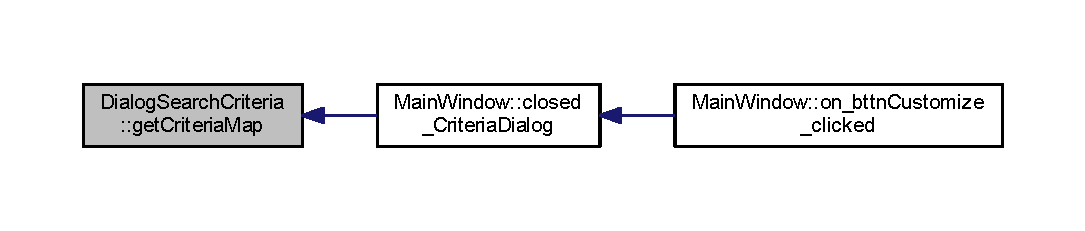
\includegraphics[width=350pt]{class_dialog_search_criteria_a4580f445b0386b977d30694afd0d0c22_icgraph}
\end{center}
\end{figure}


\hypertarget{class_dialog_search_criteria_a874909d0b8c007695ef40120bc290157}{\index{Dialog\+Search\+Criteria@{Dialog\+Search\+Criteria}!K\+E\+Y\+\_\+\+C\+O\+D\+E@{K\+E\+Y\+\_\+\+C\+O\+D\+E}}
\index{K\+E\+Y\+\_\+\+C\+O\+D\+E@{K\+E\+Y\+\_\+\+C\+O\+D\+E}!Dialog\+Search\+Criteria@{Dialog\+Search\+Criteria}}
\subsubsection[{K\+E\+Y\+\_\+\+C\+O\+D\+E}]{\setlength{\rightskip}{0pt plus 5cm}static const Q\+String Dialog\+Search\+Criteria\+::\+K\+E\+Y\+\_\+\+C\+O\+D\+E (
\begin{DoxyParamCaption}
{}
\end{DoxyParamCaption}
)\hspace{0.3cm}{\ttfamily [inline]}, {\ttfamily [static]}}}\label{class_dialog_search_criteria_a874909d0b8c007695ef40120bc290157}


Here is the caller graph for this function\+:
\nopagebreak
\begin{figure}[H]
\begin{center}
\leavevmode
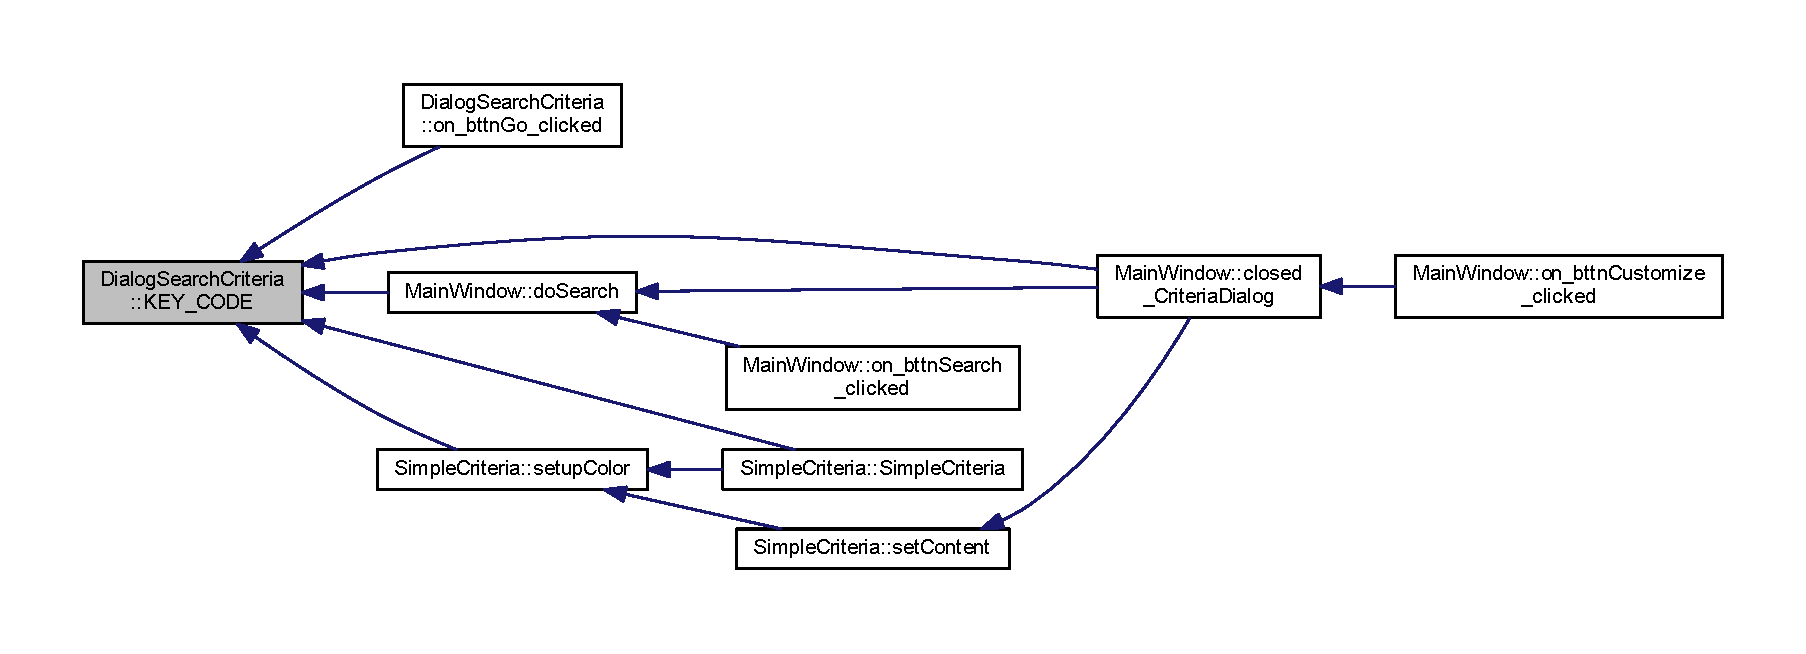
\includegraphics[width=350pt]{class_dialog_search_criteria_a874909d0b8c007695ef40120bc290157_icgraph}
\end{center}
\end{figure}


\hypertarget{class_dialog_search_criteria_a2db45b1bebeb55547c213dd558342bb7}{\index{Dialog\+Search\+Criteria@{Dialog\+Search\+Criteria}!K\+E\+Y\+\_\+\+D\+A\+T\+E@{K\+E\+Y\+\_\+\+D\+A\+T\+E}}
\index{K\+E\+Y\+\_\+\+D\+A\+T\+E@{K\+E\+Y\+\_\+\+D\+A\+T\+E}!Dialog\+Search\+Criteria@{Dialog\+Search\+Criteria}}
\subsubsection[{K\+E\+Y\+\_\+\+D\+A\+T\+E}]{\setlength{\rightskip}{0pt plus 5cm}static const Q\+String Dialog\+Search\+Criteria\+::\+K\+E\+Y\+\_\+\+D\+A\+T\+E (
\begin{DoxyParamCaption}
{}
\end{DoxyParamCaption}
)\hspace{0.3cm}{\ttfamily [inline]}, {\ttfamily [static]}}}\label{class_dialog_search_criteria_a2db45b1bebeb55547c213dd558342bb7}


Here is the caller graph for this function\+:
\nopagebreak
\begin{figure}[H]
\begin{center}
\leavevmode
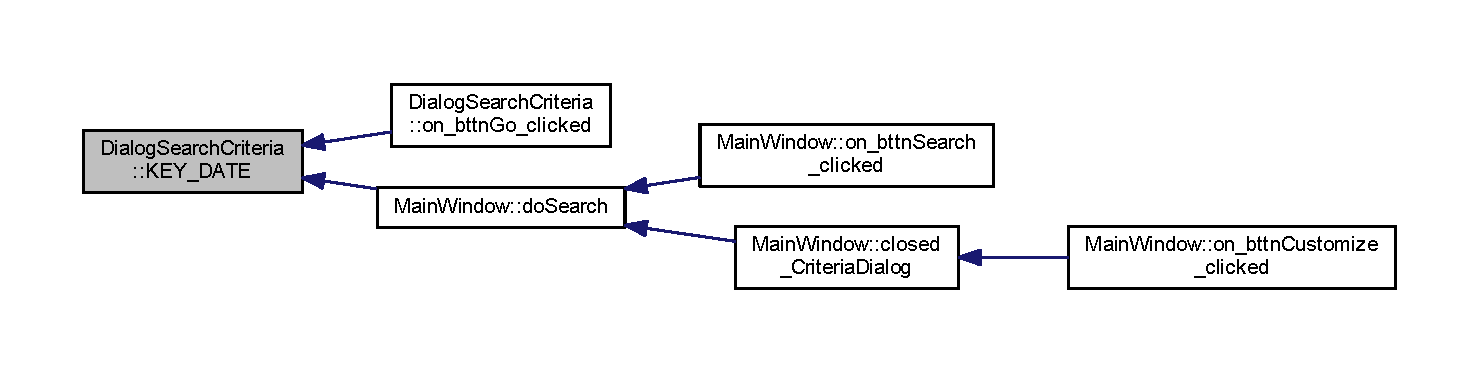
\includegraphics[width=350pt]{class_dialog_search_criteria_a2db45b1bebeb55547c213dd558342bb7_icgraph}
\end{center}
\end{figure}


\hypertarget{class_dialog_search_criteria_a8c29bb9a9d48246950ff23abee75d059}{\index{Dialog\+Search\+Criteria@{Dialog\+Search\+Criteria}!K\+E\+Y\+\_\+\+D\+E\+S\+C\+R@{K\+E\+Y\+\_\+\+D\+E\+S\+C\+R}}
\index{K\+E\+Y\+\_\+\+D\+E\+S\+C\+R@{K\+E\+Y\+\_\+\+D\+E\+S\+C\+R}!Dialog\+Search\+Criteria@{Dialog\+Search\+Criteria}}
\subsubsection[{K\+E\+Y\+\_\+\+D\+E\+S\+C\+R}]{\setlength{\rightskip}{0pt plus 5cm}static const Q\+String Dialog\+Search\+Criteria\+::\+K\+E\+Y\+\_\+\+D\+E\+S\+C\+R (
\begin{DoxyParamCaption}
{}
\end{DoxyParamCaption}
)\hspace{0.3cm}{\ttfamily [inline]}, {\ttfamily [static]}}}\label{class_dialog_search_criteria_a8c29bb9a9d48246950ff23abee75d059}


Here is the caller graph for this function\+:
\nopagebreak
\begin{figure}[H]
\begin{center}
\leavevmode
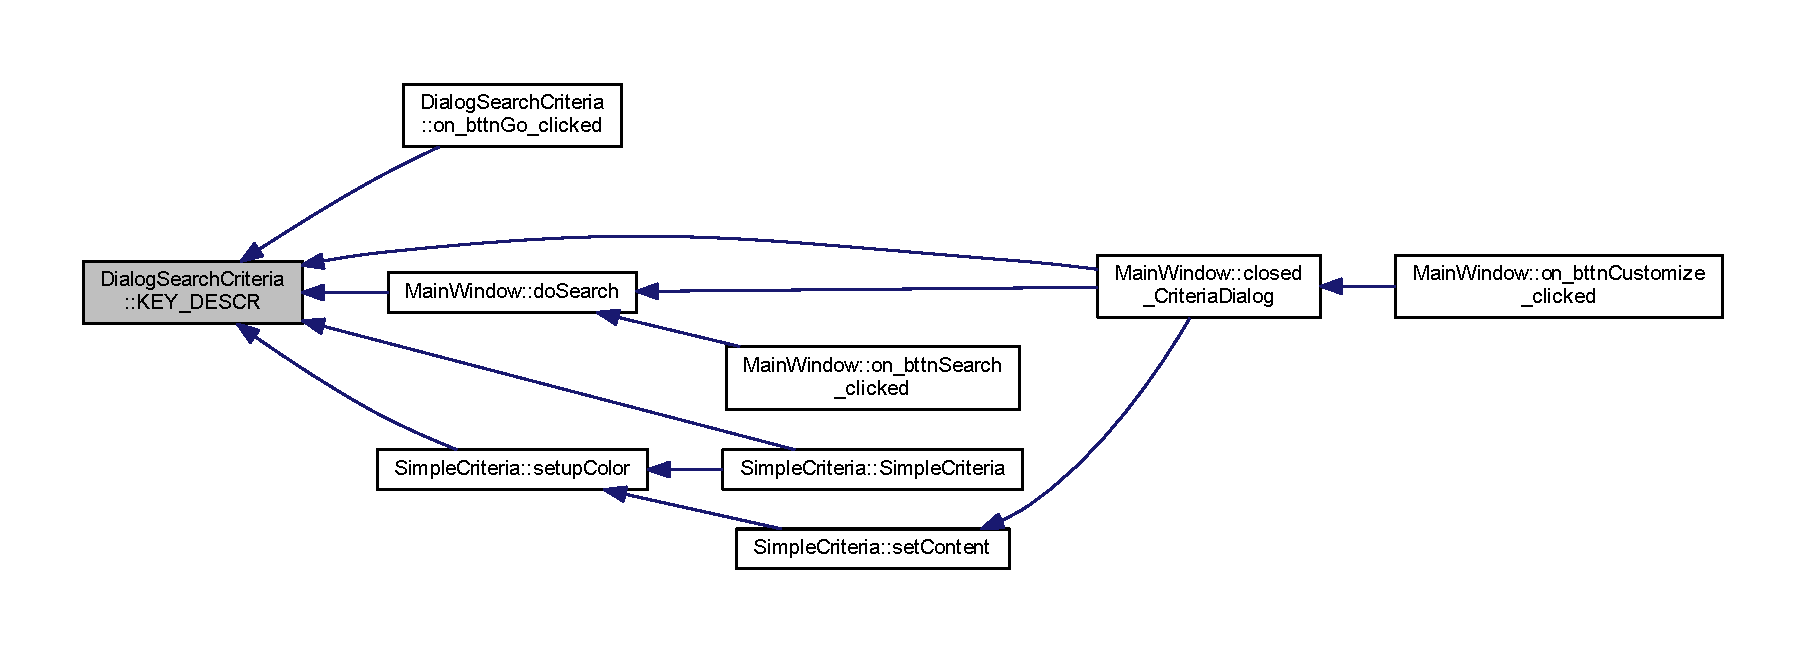
\includegraphics[width=350pt]{class_dialog_search_criteria_a8c29bb9a9d48246950ff23abee75d059_icgraph}
\end{center}
\end{figure}


\hypertarget{class_dialog_search_criteria_a3f9f43120bea93348999826e4071310d}{\index{Dialog\+Search\+Criteria@{Dialog\+Search\+Criteria}!K\+E\+Y\+\_\+\+L\+A\+N\+G\+U\+A\+G\+E@{K\+E\+Y\+\_\+\+L\+A\+N\+G\+U\+A\+G\+E}}
\index{K\+E\+Y\+\_\+\+L\+A\+N\+G\+U\+A\+G\+E@{K\+E\+Y\+\_\+\+L\+A\+N\+G\+U\+A\+G\+E}!Dialog\+Search\+Criteria@{Dialog\+Search\+Criteria}}
\subsubsection[{K\+E\+Y\+\_\+\+L\+A\+N\+G\+U\+A\+G\+E}]{\setlength{\rightskip}{0pt plus 5cm}static const Q\+String Dialog\+Search\+Criteria\+::\+K\+E\+Y\+\_\+\+L\+A\+N\+G\+U\+A\+G\+E (
\begin{DoxyParamCaption}
{}
\end{DoxyParamCaption}
)\hspace{0.3cm}{\ttfamily [inline]}, {\ttfamily [static]}}}\label{class_dialog_search_criteria_a3f9f43120bea93348999826e4071310d}


Here is the caller graph for this function\+:
\nopagebreak
\begin{figure}[H]
\begin{center}
\leavevmode
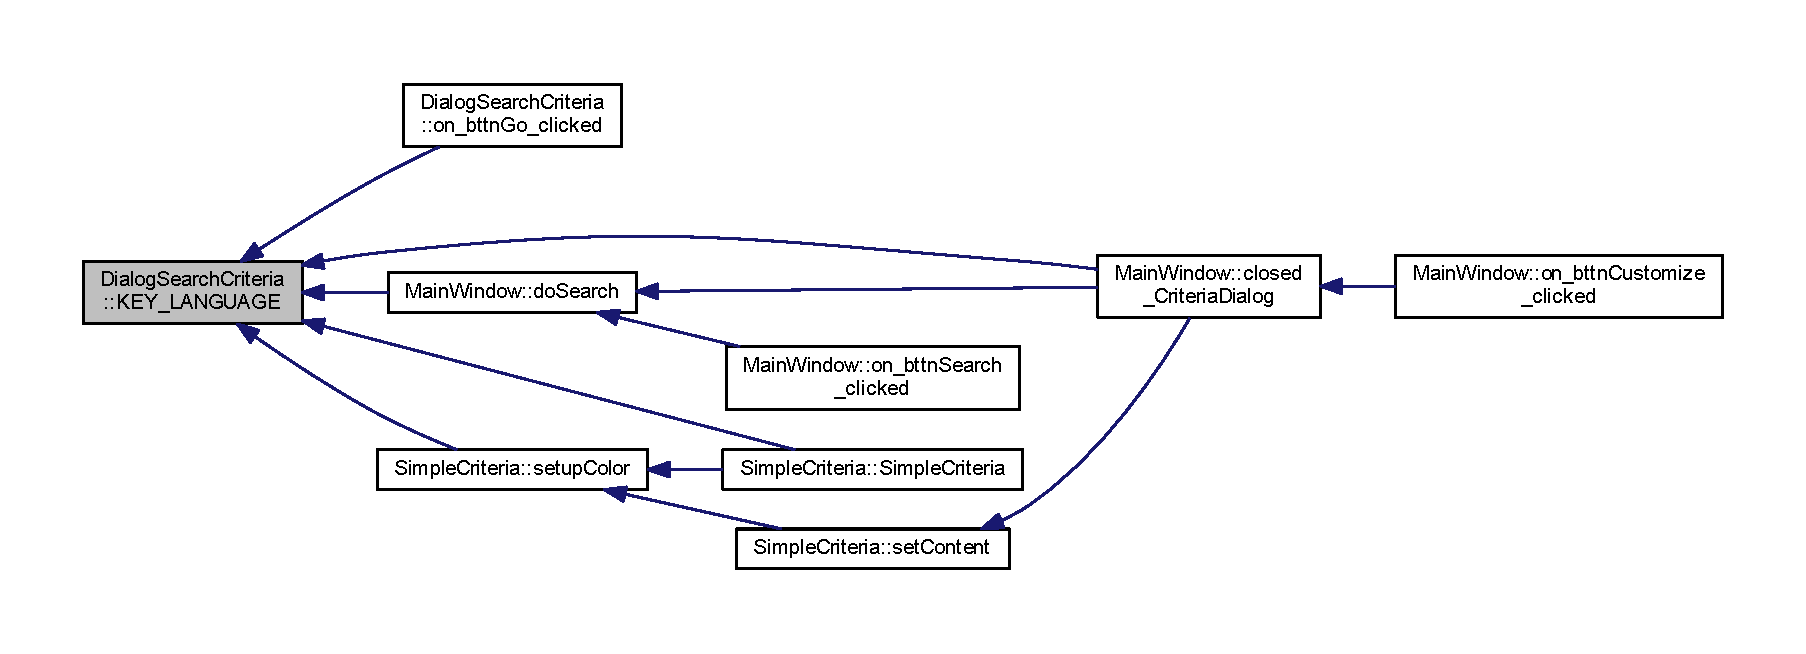
\includegraphics[width=350pt]{class_dialog_search_criteria_a3f9f43120bea93348999826e4071310d_icgraph}
\end{center}
\end{figure}


\hypertarget{class_dialog_search_criteria_ac49318706a518f848fe9b4902c120e8d}{\index{Dialog\+Search\+Criteria@{Dialog\+Search\+Criteria}!K\+E\+Y\+\_\+\+N\+A\+M\+E\+\_\+\+A\+U\+T\+H\+O\+R@{K\+E\+Y\+\_\+\+N\+A\+M\+E\+\_\+\+A\+U\+T\+H\+O\+R}}
\index{K\+E\+Y\+\_\+\+N\+A\+M\+E\+\_\+\+A\+U\+T\+H\+O\+R@{K\+E\+Y\+\_\+\+N\+A\+M\+E\+\_\+\+A\+U\+T\+H\+O\+R}!Dialog\+Search\+Criteria@{Dialog\+Search\+Criteria}}
\subsubsection[{K\+E\+Y\+\_\+\+N\+A\+M\+E\+\_\+\+A\+U\+T\+H\+O\+R}]{\setlength{\rightskip}{0pt plus 5cm}static const Q\+String Dialog\+Search\+Criteria\+::\+K\+E\+Y\+\_\+\+N\+A\+M\+E\+\_\+\+A\+U\+T\+H\+O\+R (
\begin{DoxyParamCaption}
{}
\end{DoxyParamCaption}
)\hspace{0.3cm}{\ttfamily [inline]}, {\ttfamily [static]}}}\label{class_dialog_search_criteria_ac49318706a518f848fe9b4902c120e8d}


Here is the caller graph for this function\+:
\nopagebreak
\begin{figure}[H]
\begin{center}
\leavevmode
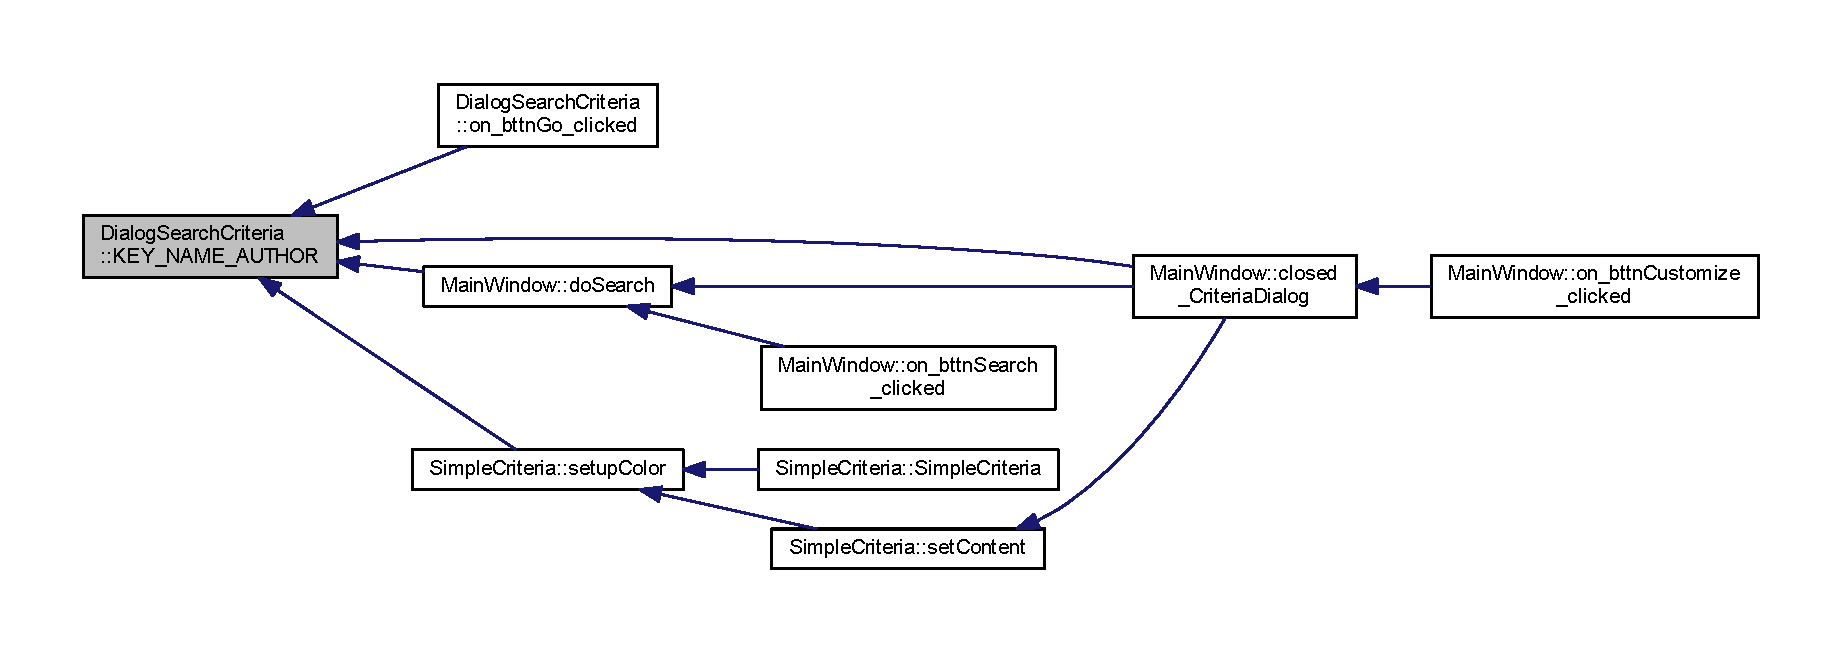
\includegraphics[width=350pt]{class_dialog_search_criteria_ac49318706a518f848fe9b4902c120e8d_icgraph}
\end{center}
\end{figure}


\hypertarget{class_dialog_search_criteria_a9b57352b785dc4b716e171c7835b0ff8}{\index{Dialog\+Search\+Criteria@{Dialog\+Search\+Criteria}!K\+E\+Y\+\_\+\+N\+A\+M\+E\+\_\+\+E\+N\+T\+R\+Y@{K\+E\+Y\+\_\+\+N\+A\+M\+E\+\_\+\+E\+N\+T\+R\+Y}}
\index{K\+E\+Y\+\_\+\+N\+A\+M\+E\+\_\+\+E\+N\+T\+R\+Y@{K\+E\+Y\+\_\+\+N\+A\+M\+E\+\_\+\+E\+N\+T\+R\+Y}!Dialog\+Search\+Criteria@{Dialog\+Search\+Criteria}}
\subsubsection[{K\+E\+Y\+\_\+\+N\+A\+M\+E\+\_\+\+E\+N\+T\+R\+Y}]{\setlength{\rightskip}{0pt plus 5cm}static const Q\+String Dialog\+Search\+Criteria\+::\+K\+E\+Y\+\_\+\+N\+A\+M\+E\+\_\+\+E\+N\+T\+R\+Y (
\begin{DoxyParamCaption}
{}
\end{DoxyParamCaption}
)\hspace{0.3cm}{\ttfamily [inline]}, {\ttfamily [static]}}}\label{class_dialog_search_criteria_a9b57352b785dc4b716e171c7835b0ff8}


Here is the caller graph for this function\+:
\nopagebreak
\begin{figure}[H]
\begin{center}
\leavevmode
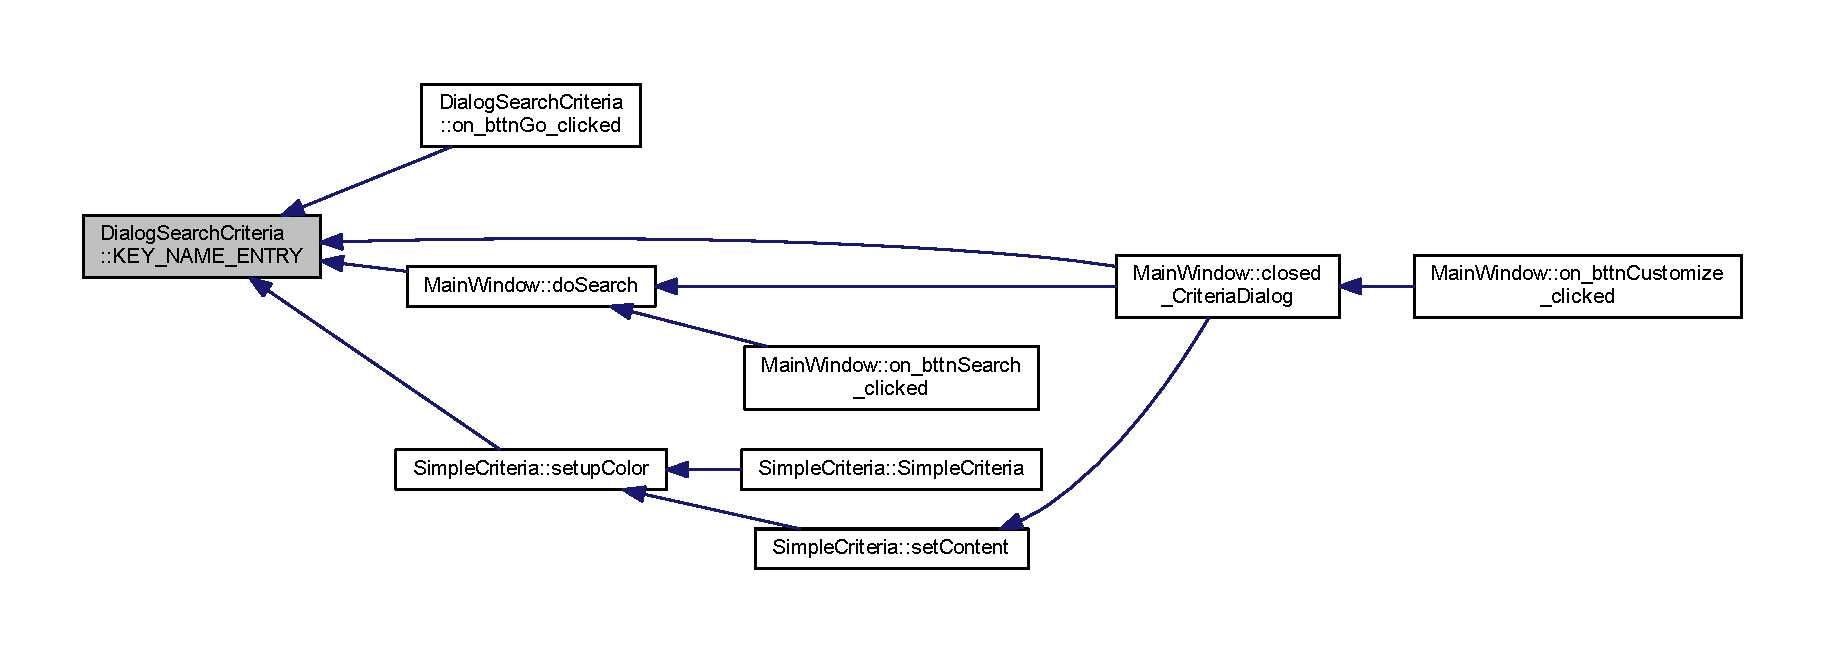
\includegraphics[width=350pt]{class_dialog_search_criteria_a9b57352b785dc4b716e171c7835b0ff8_icgraph}
\end{center}
\end{figure}


\hypertarget{class_dialog_search_criteria_a855feb356d17d2631bf7251f1a501ce1}{\index{Dialog\+Search\+Criteria@{Dialog\+Search\+Criteria}!K\+E\+Y\+\_\+\+P\+A\+T\+T\+E\+R\+N@{K\+E\+Y\+\_\+\+P\+A\+T\+T\+E\+R\+N}}
\index{K\+E\+Y\+\_\+\+P\+A\+T\+T\+E\+R\+N@{K\+E\+Y\+\_\+\+P\+A\+T\+T\+E\+R\+N}!Dialog\+Search\+Criteria@{Dialog\+Search\+Criteria}}
\subsubsection[{K\+E\+Y\+\_\+\+P\+A\+T\+T\+E\+R\+N}]{\setlength{\rightskip}{0pt plus 5cm}static const Q\+String Dialog\+Search\+Criteria\+::\+K\+E\+Y\+\_\+\+P\+A\+T\+T\+E\+R\+N (
\begin{DoxyParamCaption}
{}
\end{DoxyParamCaption}
)\hspace{0.3cm}{\ttfamily [inline]}, {\ttfamily [static]}}}\label{class_dialog_search_criteria_a855feb356d17d2631bf7251f1a501ce1}


Here is the caller graph for this function\+:
\nopagebreak
\begin{figure}[H]
\begin{center}
\leavevmode
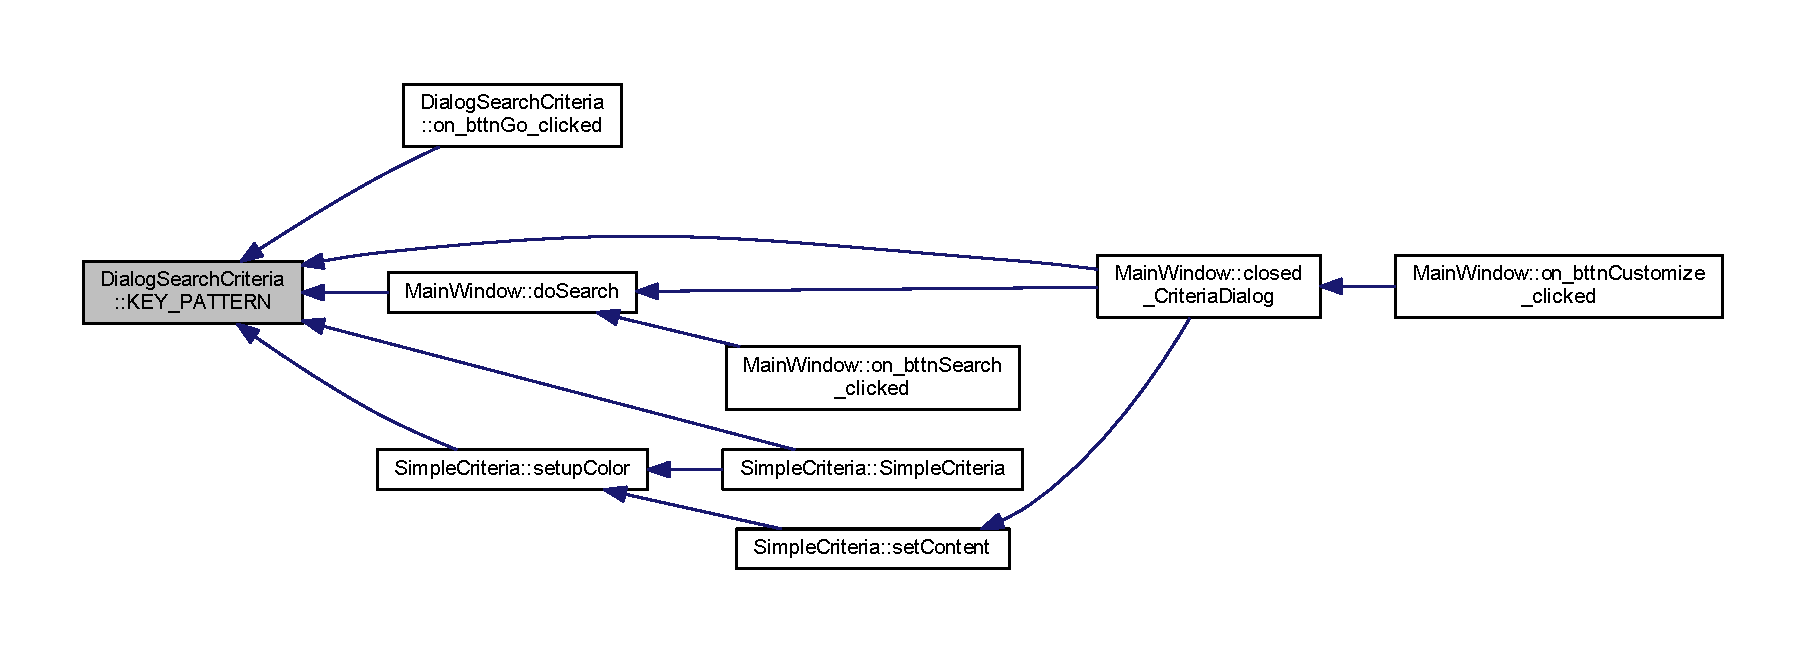
\includegraphics[width=350pt]{class_dialog_search_criteria_a855feb356d17d2631bf7251f1a501ce1_icgraph}
\end{center}
\end{figure}


\hypertarget{class_dialog_search_criteria_a0e106dc53e15508c8d8bf59308870371}{\index{Dialog\+Search\+Criteria@{Dialog\+Search\+Criteria}!on\+\_\+bttn\+Go\+\_\+clicked@{on\+\_\+bttn\+Go\+\_\+clicked}}
\index{on\+\_\+bttn\+Go\+\_\+clicked@{on\+\_\+bttn\+Go\+\_\+clicked}!Dialog\+Search\+Criteria@{Dialog\+Search\+Criteria}}
\subsubsection[{on\+\_\+bttn\+Go\+\_\+clicked}]{\setlength{\rightskip}{0pt plus 5cm}void Dialog\+Search\+Criteria\+::on\+\_\+bttn\+Go\+\_\+clicked (
\begin{DoxyParamCaption}
{}
\end{DoxyParamCaption}
)\hspace{0.3cm}{\ttfamily [private]}, {\ttfamily [slot]}}}\label{class_dialog_search_criteria_a0e106dc53e15508c8d8bf59308870371}


\hyperlink{class_dialog_search_criteria_a0e106dc53e15508c8d8bf59308870371}{Dialog\+Search\+Criteria\+::on\+\_\+bttn\+Go\+\_\+clicked}. 

Retrieves all the inserted information, saves it into a Hash\+Map and closes the dialog. 

Here is the call graph for this function\+:
\nopagebreak
\begin{figure}[H]
\begin{center}
\leavevmode
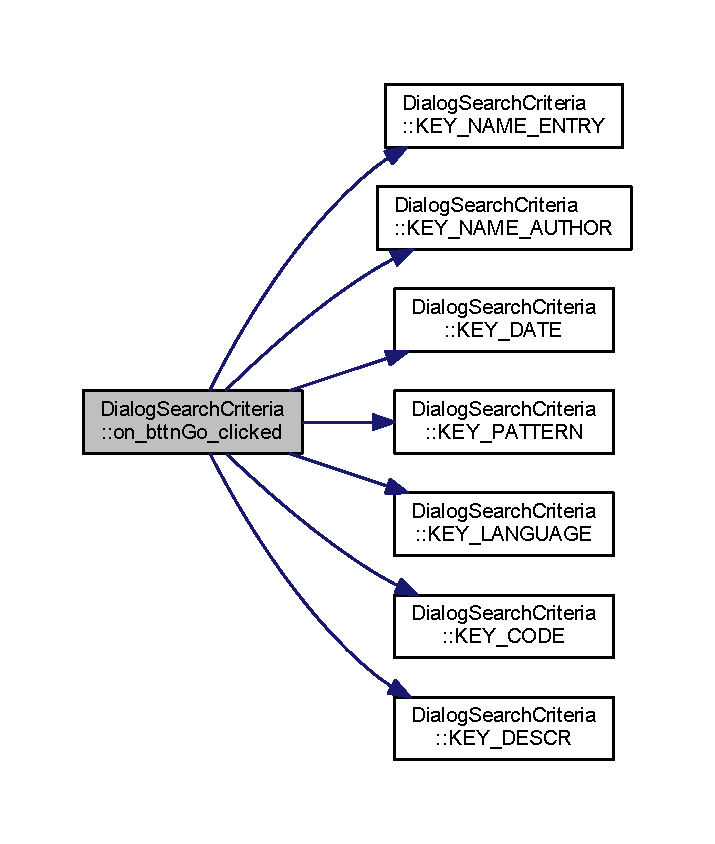
\includegraphics[width=343pt]{class_dialog_search_criteria_a0e106dc53e15508c8d8bf59308870371_cgraph}
\end{center}
\end{figure}




\subsection{Member Data Documentation}
\hypertarget{class_dialog_search_criteria_a3ed8b9ec17d79f4e995926e2ba7e02b4}{\index{Dialog\+Search\+Criteria@{Dialog\+Search\+Criteria}!criteria\+Map@{criteria\+Map}}
\index{criteria\+Map@{criteria\+Map}!Dialog\+Search\+Criteria@{Dialog\+Search\+Criteria}}
\subsubsection[{criteria\+Map}]{\setlength{\rightskip}{0pt plus 5cm}Q\+Multi\+Map$<$Q\+String, Q\+String$>$ Dialog\+Search\+Criteria\+::criteria\+Map\hspace{0.3cm}{\ttfamily [private]}}}\label{class_dialog_search_criteria_a3ed8b9ec17d79f4e995926e2ba7e02b4}
\hypertarget{class_dialog_search_criteria_a7e7d05c4b1937aec851d514e19182c50}{\index{Dialog\+Search\+Criteria@{Dialog\+Search\+Criteria}!ui@{ui}}
\index{ui@{ui}!Dialog\+Search\+Criteria@{Dialog\+Search\+Criteria}}
\subsubsection[{ui}]{\setlength{\rightskip}{0pt plus 5cm}Ui\+::\+Dialog\+Search\+Criteria$\ast$ Dialog\+Search\+Criteria\+::ui\hspace{0.3cm}{\ttfamily [private]}}}\label{class_dialog_search_criteria_a7e7d05c4b1937aec851d514e19182c50}


The documentation for this class was generated from the following files\+:\begin{DoxyCompactItemize}
\item 
D\+:/\+Entwicklung/\+C++/\+Workspace/\+Beleg\+Cpp/\hyperlink{dialogsearchcriteria_8h}{dialogsearchcriteria.\+h}\item 
D\+:/\+Entwicklung/\+C++/\+Workspace/\+Beleg\+Cpp/\hyperlink{dialogsearchcriteria_8cpp}{dialogsearchcriteria.\+cpp}\end{DoxyCompactItemize}

\hypertarget{class_dialog_settings}{\section{Dialog\+Settings Class Reference}
\label{class_dialog_settings}\index{Dialog\+Settings@{Dialog\+Settings}}
}


The \hyperlink{class_dialog_settings}{Dialog\+Settings} class.  




{\ttfamily \#include $<$dialogsettings.\+h$>$}



Inheritance diagram for Dialog\+Settings\+:
\nopagebreak
\begin{figure}[H]
\begin{center}
\leavevmode
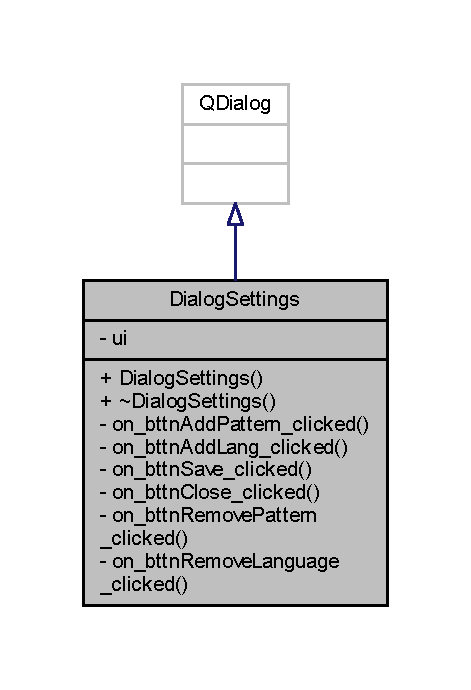
\includegraphics[width=226pt]{class_dialog_settings__inherit__graph}
\end{center}
\end{figure}


Collaboration diagram for Dialog\+Settings\+:
\nopagebreak
\begin{figure}[H]
\begin{center}
\leavevmode
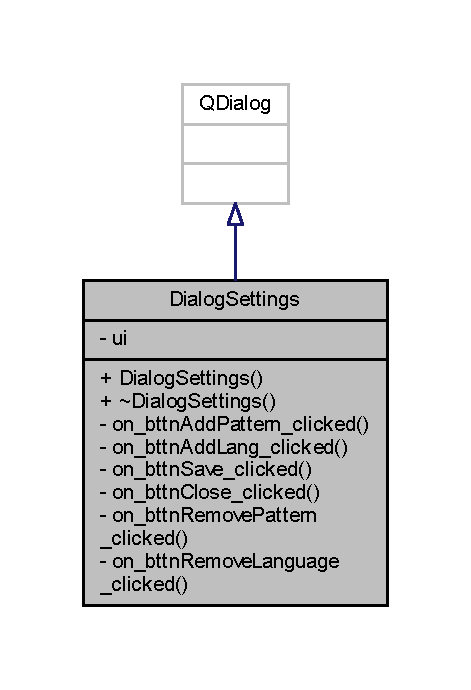
\includegraphics[width=226pt]{class_dialog_settings__coll__graph}
\end{center}
\end{figure}
\subsection*{Public Member Functions}
\begin{DoxyCompactItemize}
\item 
\hyperlink{class_dialog_settings_afd62a031c10ddfa1fc50f8f5ade07db4}{Dialog\+Settings} (Q\+Widget $\ast$parent=0)
\begin{DoxyCompactList}\small\item\em \hyperlink{class_dialog_settings_afd62a031c10ddfa1fc50f8f5ade07db4}{Dialog\+Settings\+::\+Dialog\+Settings}. \end{DoxyCompactList}\item 
\hyperlink{class_dialog_settings_a10e028cc22f2ab2367f582242fd8115e}{$\sim$\+Dialog\+Settings} ()
\begin{DoxyCompactList}\small\item\em \hyperlink{class_dialog_settings_a10e028cc22f2ab2367f582242fd8115e}{Dialog\+Settings\+::$\sim$\+Dialog\+Settings}. \end{DoxyCompactList}\end{DoxyCompactItemize}
\subsection*{Private Slots}
\begin{DoxyCompactItemize}
\item 
void \hyperlink{class_dialog_settings_a787f686519f7877b35a330e584965c5c}{on\+\_\+bttn\+Add\+Pattern\+\_\+clicked} ()
\begin{DoxyCompactList}\small\item\em \hyperlink{class_dialog_settings_a787f686519f7877b35a330e584965c5c}{Dialog\+Settings\+::on\+\_\+bttn\+Add\+Pattern\+\_\+clicked}. \end{DoxyCompactList}\item 
void \hyperlink{class_dialog_settings_a90c6372109b546601f37e694552158a4}{on\+\_\+bttn\+Add\+Lang\+\_\+clicked} ()
\begin{DoxyCompactList}\small\item\em \hyperlink{class_dialog_settings_a787f686519f7877b35a330e584965c5c}{Dialog\+Settings\+::on\+\_\+bttn\+Add\+Pattern\+\_\+clicked}. \end{DoxyCompactList}\item 
void \hyperlink{class_dialog_settings_a04ff2f5547ff8e6b4725664153ff227f}{on\+\_\+bttn\+Save\+\_\+clicked} ()
\begin{DoxyCompactList}\small\item\em \hyperlink{class_dialog_settings_a04ff2f5547ff8e6b4725664153ff227f}{Dialog\+Settings\+::on\+\_\+bttn\+Save\+\_\+clicked}. \end{DoxyCompactList}\item 
void \hyperlink{class_dialog_settings_af5046dffc64be390d766fa3bcd894a42}{on\+\_\+bttn\+Close\+\_\+clicked} ()
\begin{DoxyCompactList}\small\item\em \hyperlink{class_dialog_settings_af5046dffc64be390d766fa3bcd894a42}{Dialog\+Settings\+::on\+\_\+bttn\+Close\+\_\+clicked}. \end{DoxyCompactList}\item 
void \hyperlink{class_dialog_settings_a32f59e49086e1c86e4a11eb883cc81dd}{on\+\_\+bttn\+Remove\+Pattern\+\_\+clicked} ()
\begin{DoxyCompactList}\small\item\em \hyperlink{class_dialog_settings_a32f59e49086e1c86e4a11eb883cc81dd}{Dialog\+Settings\+::on\+\_\+bttn\+Remove\+Pattern\+\_\+clicked}. \end{DoxyCompactList}\item 
void \hyperlink{class_dialog_settings_a37b337f965d8794d13235ff79ea54cce}{on\+\_\+bttn\+Remove\+Language\+\_\+clicked} ()
\begin{DoxyCompactList}\small\item\em \hyperlink{class_dialog_settings_a37b337f965d8794d13235ff79ea54cce}{Dialog\+Settings\+::on\+\_\+bttn\+Remove\+Language\+\_\+clicked}. \end{DoxyCompactList}\end{DoxyCompactItemize}
\subsection*{Private Attributes}
\begin{DoxyCompactItemize}
\item 
Ui\+::\+Dialog\+Settings $\ast$ \hyperlink{class_dialog_settings_a5b53d91a27cdf68f77e4bdd10b6a9bba}{ui}
\end{DoxyCompactItemize}


\subsection{Detailed Description}
The \hyperlink{class_dialog_settings}{Dialog\+Settings} class. 

This class represents the Q\+Dialog for the settings.

\begin{DoxyAuthor}{Author}
Robert Wolfinger 
\end{DoxyAuthor}
\begin{DoxyVersion}{Version}
1.\+0 20.\+09.\+14 
\end{DoxyVersion}


\subsection{Constructor \& Destructor Documentation}
\hypertarget{class_dialog_settings_afd62a031c10ddfa1fc50f8f5ade07db4}{\index{Dialog\+Settings@{Dialog\+Settings}!Dialog\+Settings@{Dialog\+Settings}}
\index{Dialog\+Settings@{Dialog\+Settings}!Dialog\+Settings@{Dialog\+Settings}}
\subsubsection[{Dialog\+Settings}]{\setlength{\rightskip}{0pt plus 5cm}Dialog\+Settings\+::\+Dialog\+Settings (
\begin{DoxyParamCaption}
\item[{Q\+Widget $\ast$}]{parent = {\ttfamily 0}}
\end{DoxyParamCaption}
)\hspace{0.3cm}{\ttfamily [explicit]}}}\label{class_dialog_settings_afd62a031c10ddfa1fc50f8f5ade07db4}


\hyperlink{class_dialog_settings_afd62a031c10ddfa1fc50f8f5ade07db4}{Dialog\+Settings\+::\+Dialog\+Settings}. 

\begin{DoxyAuthor}{Author}
Robert Wolfinger 
\end{DoxyAuthor}
\begin{DoxyVersion}{Version}
1.\+0 20.\+09.\+14 Constructs the dialog. Retrieves all languages and patterns from the database and adds them to the dialog.
\end{DoxyVersion}

\begin{DoxyParams}{Parameters}
{\em parent} & \\
\hline
\end{DoxyParams}


Here is the call graph for this function\+:\nopagebreak
\begin{figure}[H]
\begin{center}
\leavevmode
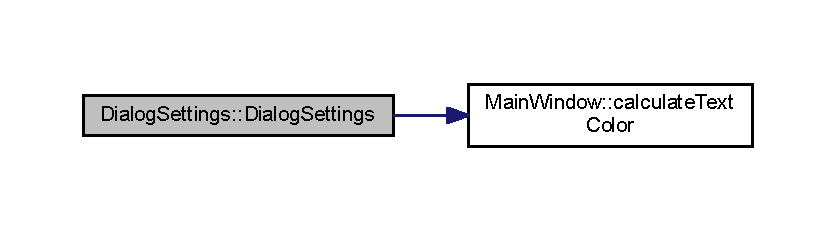
\includegraphics[width=350pt]{class_dialog_settings_afd62a031c10ddfa1fc50f8f5ade07db4_cgraph}
\end{center}
\end{figure}


\hypertarget{class_dialog_settings_a10e028cc22f2ab2367f582242fd8115e}{\index{Dialog\+Settings@{Dialog\+Settings}!````~Dialog\+Settings@{$\sim$\+Dialog\+Settings}}
\index{````~Dialog\+Settings@{$\sim$\+Dialog\+Settings}!Dialog\+Settings@{Dialog\+Settings}}
\subsubsection[{$\sim$\+Dialog\+Settings}]{\setlength{\rightskip}{0pt plus 5cm}Dialog\+Settings\+::$\sim$\+Dialog\+Settings (
\begin{DoxyParamCaption}
{}
\end{DoxyParamCaption}
)}}\label{class_dialog_settings_a10e028cc22f2ab2367f582242fd8115e}


\hyperlink{class_dialog_settings_a10e028cc22f2ab2367f582242fd8115e}{Dialog\+Settings\+::$\sim$\+Dialog\+Settings}. 

Deconstructs the dialog 

\subsection{Member Function Documentation}
\hypertarget{class_dialog_settings_a90c6372109b546601f37e694552158a4}{\index{Dialog\+Settings@{Dialog\+Settings}!on\+\_\+bttn\+Add\+Lang\+\_\+clicked@{on\+\_\+bttn\+Add\+Lang\+\_\+clicked}}
\index{on\+\_\+bttn\+Add\+Lang\+\_\+clicked@{on\+\_\+bttn\+Add\+Lang\+\_\+clicked}!Dialog\+Settings@{Dialog\+Settings}}
\subsubsection[{on\+\_\+bttn\+Add\+Lang\+\_\+clicked}]{\setlength{\rightskip}{0pt plus 5cm}void Dialog\+Settings\+::on\+\_\+bttn\+Add\+Lang\+\_\+clicked (
\begin{DoxyParamCaption}
{}
\end{DoxyParamCaption}
)\hspace{0.3cm}{\ttfamily [private]}, {\ttfamily [slot]}}}\label{class_dialog_settings_a90c6372109b546601f37e694552158a4}


\hyperlink{class_dialog_settings_a787f686519f7877b35a330e584965c5c}{Dialog\+Settings\+::on\+\_\+bttn\+Add\+Pattern\+\_\+clicked}. 

Opens the dialog to add a language and if submitted adds the language to the Q\+List\+Widget. 

Here is the call graph for this function\+:
\nopagebreak
\begin{figure}[H]
\begin{center}
\leavevmode
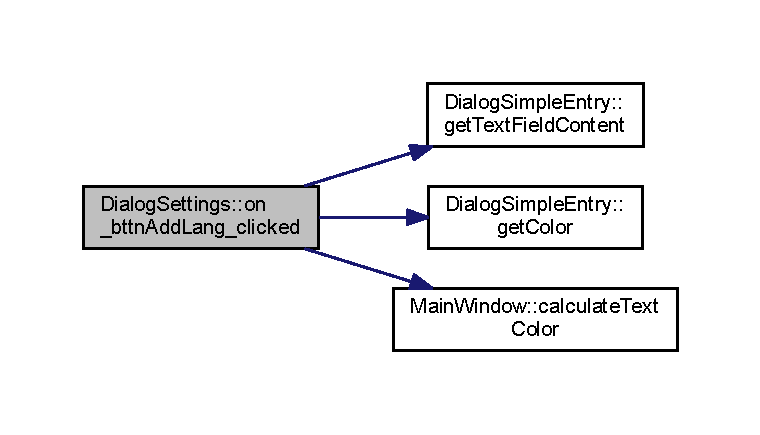
\includegraphics[width=350pt]{class_dialog_settings_a90c6372109b546601f37e694552158a4_cgraph}
\end{center}
\end{figure}


\hypertarget{class_dialog_settings_a787f686519f7877b35a330e584965c5c}{\index{Dialog\+Settings@{Dialog\+Settings}!on\+\_\+bttn\+Add\+Pattern\+\_\+clicked@{on\+\_\+bttn\+Add\+Pattern\+\_\+clicked}}
\index{on\+\_\+bttn\+Add\+Pattern\+\_\+clicked@{on\+\_\+bttn\+Add\+Pattern\+\_\+clicked}!Dialog\+Settings@{Dialog\+Settings}}
\subsubsection[{on\+\_\+bttn\+Add\+Pattern\+\_\+clicked}]{\setlength{\rightskip}{0pt plus 5cm}void Dialog\+Settings\+::on\+\_\+bttn\+Add\+Pattern\+\_\+clicked (
\begin{DoxyParamCaption}
{}
\end{DoxyParamCaption}
)\hspace{0.3cm}{\ttfamily [private]}, {\ttfamily [slot]}}}\label{class_dialog_settings_a787f686519f7877b35a330e584965c5c}


\hyperlink{class_dialog_settings_a787f686519f7877b35a330e584965c5c}{Dialog\+Settings\+::on\+\_\+bttn\+Add\+Pattern\+\_\+clicked}. 

Opens the dialog to add a pattern and if submitted adds the pattern to the Q\+List\+Widget. 

Here is the call graph for this function\+:
\nopagebreak
\begin{figure}[H]
\begin{center}
\leavevmode
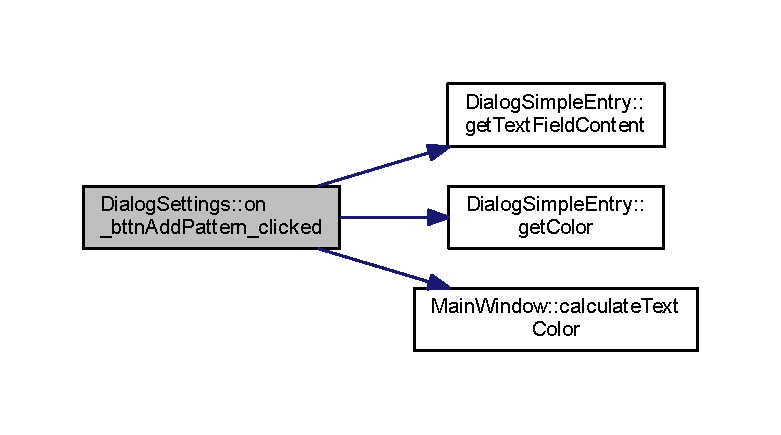
\includegraphics[width=350pt]{class_dialog_settings_a787f686519f7877b35a330e584965c5c_cgraph}
\end{center}
\end{figure}


\hypertarget{class_dialog_settings_af5046dffc64be390d766fa3bcd894a42}{\index{Dialog\+Settings@{Dialog\+Settings}!on\+\_\+bttn\+Close\+\_\+clicked@{on\+\_\+bttn\+Close\+\_\+clicked}}
\index{on\+\_\+bttn\+Close\+\_\+clicked@{on\+\_\+bttn\+Close\+\_\+clicked}!Dialog\+Settings@{Dialog\+Settings}}
\subsubsection[{on\+\_\+bttn\+Close\+\_\+clicked}]{\setlength{\rightskip}{0pt plus 5cm}void Dialog\+Settings\+::on\+\_\+bttn\+Close\+\_\+clicked (
\begin{DoxyParamCaption}
{}
\end{DoxyParamCaption}
)\hspace{0.3cm}{\ttfamily [private]}, {\ttfamily [slot]}}}\label{class_dialog_settings_af5046dffc64be390d766fa3bcd894a42}


\hyperlink{class_dialog_settings_af5046dffc64be390d766fa3bcd894a42}{Dialog\+Settings\+::on\+\_\+bttn\+Close\+\_\+clicked}. 

Closes the dialog. \hypertarget{class_dialog_settings_a37b337f965d8794d13235ff79ea54cce}{\index{Dialog\+Settings@{Dialog\+Settings}!on\+\_\+bttn\+Remove\+Language\+\_\+clicked@{on\+\_\+bttn\+Remove\+Language\+\_\+clicked}}
\index{on\+\_\+bttn\+Remove\+Language\+\_\+clicked@{on\+\_\+bttn\+Remove\+Language\+\_\+clicked}!Dialog\+Settings@{Dialog\+Settings}}
\subsubsection[{on\+\_\+bttn\+Remove\+Language\+\_\+clicked}]{\setlength{\rightskip}{0pt plus 5cm}void Dialog\+Settings\+::on\+\_\+bttn\+Remove\+Language\+\_\+clicked (
\begin{DoxyParamCaption}
{}
\end{DoxyParamCaption}
)\hspace{0.3cm}{\ttfamily [private]}, {\ttfamily [slot]}}}\label{class_dialog_settings_a37b337f965d8794d13235ff79ea54cce}


\hyperlink{class_dialog_settings_a37b337f965d8794d13235ff79ea54cce}{Dialog\+Settings\+::on\+\_\+bttn\+Remove\+Language\+\_\+clicked}. 

Removes all selected languages from the Q\+List\+Widget. \hypertarget{class_dialog_settings_a32f59e49086e1c86e4a11eb883cc81dd}{\index{Dialog\+Settings@{Dialog\+Settings}!on\+\_\+bttn\+Remove\+Pattern\+\_\+clicked@{on\+\_\+bttn\+Remove\+Pattern\+\_\+clicked}}
\index{on\+\_\+bttn\+Remove\+Pattern\+\_\+clicked@{on\+\_\+bttn\+Remove\+Pattern\+\_\+clicked}!Dialog\+Settings@{Dialog\+Settings}}
\subsubsection[{on\+\_\+bttn\+Remove\+Pattern\+\_\+clicked}]{\setlength{\rightskip}{0pt plus 5cm}void Dialog\+Settings\+::on\+\_\+bttn\+Remove\+Pattern\+\_\+clicked (
\begin{DoxyParamCaption}
{}
\end{DoxyParamCaption}
)\hspace{0.3cm}{\ttfamily [private]}, {\ttfamily [slot]}}}\label{class_dialog_settings_a32f59e49086e1c86e4a11eb883cc81dd}


\hyperlink{class_dialog_settings_a32f59e49086e1c86e4a11eb883cc81dd}{Dialog\+Settings\+::on\+\_\+bttn\+Remove\+Pattern\+\_\+clicked}. 

Removes all selected patterns from the Q\+List\+Widget. \hypertarget{class_dialog_settings_a04ff2f5547ff8e6b4725664153ff227f}{\index{Dialog\+Settings@{Dialog\+Settings}!on\+\_\+bttn\+Save\+\_\+clicked@{on\+\_\+bttn\+Save\+\_\+clicked}}
\index{on\+\_\+bttn\+Save\+\_\+clicked@{on\+\_\+bttn\+Save\+\_\+clicked}!Dialog\+Settings@{Dialog\+Settings}}
\subsubsection[{on\+\_\+bttn\+Save\+\_\+clicked}]{\setlength{\rightskip}{0pt plus 5cm}void Dialog\+Settings\+::on\+\_\+bttn\+Save\+\_\+clicked (
\begin{DoxyParamCaption}
{}
\end{DoxyParamCaption}
)\hspace{0.3cm}{\ttfamily [private]}, {\ttfamily [slot]}}}\label{class_dialog_settings_a04ff2f5547ff8e6b4725664153ff227f}


\hyperlink{class_dialog_settings_a04ff2f5547ff8e6b4725664153ff227f}{Dialog\+Settings\+::on\+\_\+bttn\+Save\+\_\+clicked}. 

Saves all items in the Q\+List\+Widget to the database.

T\+O\+D\+O All entries in the table are first deleted and then all items are saved. Not the most efficient way... This has to be reworked. 

\subsection{Member Data Documentation}
\hypertarget{class_dialog_settings_a5b53d91a27cdf68f77e4bdd10b6a9bba}{\index{Dialog\+Settings@{Dialog\+Settings}!ui@{ui}}
\index{ui@{ui}!Dialog\+Settings@{Dialog\+Settings}}
\subsubsection[{ui}]{\setlength{\rightskip}{0pt plus 5cm}Ui\+::\+Dialog\+Settings$\ast$ Dialog\+Settings\+::ui\hspace{0.3cm}{\ttfamily [private]}}}\label{class_dialog_settings_a5b53d91a27cdf68f77e4bdd10b6a9bba}


The documentation for this class was generated from the following files\+:\begin{DoxyCompactItemize}
\item 
D\+:/\+Entwicklung/\+C++/\+Workspace/\+Beleg\+Cpp/\hyperlink{dialogsettings_8h}{dialogsettings.\+h}\item 
D\+:/\+Entwicklung/\+C++/\+Workspace/\+Beleg\+Cpp/\hyperlink{dialogsettings_8cpp}{dialogsettings.\+cpp}\end{DoxyCompactItemize}

\hypertarget{class_dialog_simple_entry}{\section{Dialog\+Simple\+Entry Class Reference}
\label{class_dialog_simple_entry}\index{Dialog\+Simple\+Entry@{Dialog\+Simple\+Entry}}
}


The \hyperlink{class_dialog_simple_entry}{Dialog\+Simple\+Entry} class.  




{\ttfamily \#include $<$dialogsimpleentry.\+h$>$}



Inheritance diagram for Dialog\+Simple\+Entry\+:
\nopagebreak
\begin{figure}[H]
\begin{center}
\leavevmode
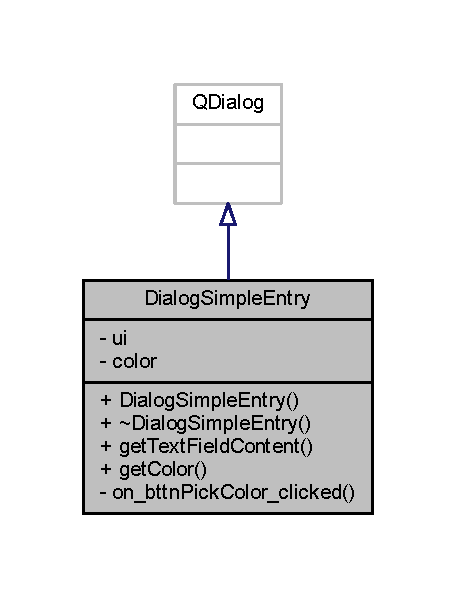
\includegraphics[width=219pt]{class_dialog_simple_entry__inherit__graph}
\end{center}
\end{figure}


Collaboration diagram for Dialog\+Simple\+Entry\+:
\nopagebreak
\begin{figure}[H]
\begin{center}
\leavevmode
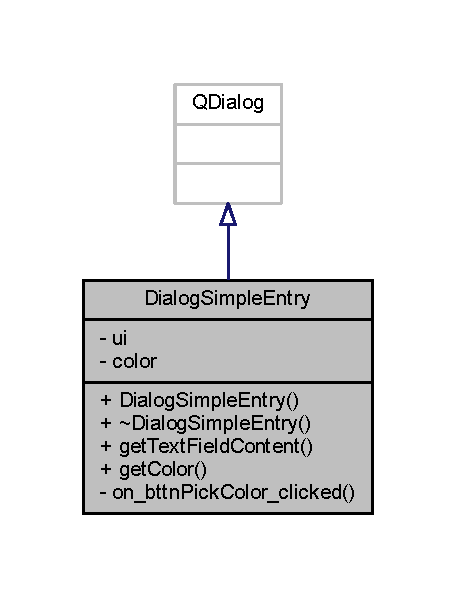
\includegraphics[width=219pt]{class_dialog_simple_entry__coll__graph}
\end{center}
\end{figure}
\subsection*{Public Member Functions}
\begin{DoxyCompactItemize}
\item 
\hyperlink{class_dialog_simple_entry_af0c71a19feee305b6e5c2e637070311a}{Dialog\+Simple\+Entry} (Q\+Widget $\ast$parent=0, Q\+String lbl\+Name=\char`\"{}Default\char`\"{})
\begin{DoxyCompactList}\small\item\em \hyperlink{class_dialog_simple_entry_af0c71a19feee305b6e5c2e637070311a}{Dialog\+Simple\+Entry\+::\+Dialog\+Simple\+Entry}. \end{DoxyCompactList}\item 
\hyperlink{class_dialog_simple_entry_a951b30da780f0409903c76f1efbd91f1}{$\sim$\+Dialog\+Simple\+Entry} ()
\begin{DoxyCompactList}\small\item\em \hyperlink{class_dialog_simple_entry_a951b30da780f0409903c76f1efbd91f1}{Dialog\+Simple\+Entry\+::$\sim$\+Dialog\+Simple\+Entry}. \end{DoxyCompactList}\item 
Q\+String \hyperlink{class_dialog_simple_entry_ab9f80cd88dae4100bfb47b9df2cd02ad}{get\+Text\+Field\+Content} ()
\begin{DoxyCompactList}\small\item\em \hyperlink{class_dialog_simple_entry_ab9f80cd88dae4100bfb47b9df2cd02ad}{Dialog\+Simple\+Entry\+::get\+Text\+Field\+Content}. \end{DoxyCompactList}\item 
Q\+Color \hyperlink{class_dialog_simple_entry_addf576d4bc4e1acbd27743c112f267b1}{get\+Color} ()
\begin{DoxyCompactList}\small\item\em \hyperlink{class_dialog_simple_entry_addf576d4bc4e1acbd27743c112f267b1}{Dialog\+Simple\+Entry\+::get\+Color}. \end{DoxyCompactList}\end{DoxyCompactItemize}
\subsection*{Private Slots}
\begin{DoxyCompactItemize}
\item 
void \hyperlink{class_dialog_simple_entry_a08da9e5b778950ec6cf3172e04d5e4b4}{on\+\_\+bttn\+Pick\+Color\+\_\+clicked} ()
\begin{DoxyCompactList}\small\item\em \hyperlink{class_dialog_simple_entry_a08da9e5b778950ec6cf3172e04d5e4b4}{Dialog\+Simple\+Entry\+::on\+\_\+bttn\+Pick\+Color\+\_\+clicked}. \end{DoxyCompactList}\end{DoxyCompactItemize}
\subsection*{Private Attributes}
\begin{DoxyCompactItemize}
\item 
Ui\+::\+Dialog\+Simple\+Entry $\ast$ \hyperlink{class_dialog_simple_entry_a3ef78d511f3bd60f104be4851b8e8e7b}{ui}
\item 
Q\+Color \hyperlink{class_dialog_simple_entry_a797fd737de17d712425cb61142a9789d}{color}
\end{DoxyCompactItemize}


\subsection{Detailed Description}
The \hyperlink{class_dialog_simple_entry}{Dialog\+Simple\+Entry} class. 

This class represents a Q\+Dialog to create one pattern or language entry.

\begin{DoxyAuthor}{Author}
Robert Wolfinger 
\end{DoxyAuthor}
\begin{DoxyVersion}{Version}
1.\+0 20.\+09.\+14 
\end{DoxyVersion}


\subsection{Constructor \& Destructor Documentation}
\hypertarget{class_dialog_simple_entry_af0c71a19feee305b6e5c2e637070311a}{\index{Dialog\+Simple\+Entry@{Dialog\+Simple\+Entry}!Dialog\+Simple\+Entry@{Dialog\+Simple\+Entry}}
\index{Dialog\+Simple\+Entry@{Dialog\+Simple\+Entry}!Dialog\+Simple\+Entry@{Dialog\+Simple\+Entry}}
\subsubsection[{Dialog\+Simple\+Entry}]{\setlength{\rightskip}{0pt plus 5cm}Dialog\+Simple\+Entry\+::\+Dialog\+Simple\+Entry (
\begin{DoxyParamCaption}
\item[{Q\+Widget $\ast$}]{parent = {\ttfamily 0}, }
\item[{Q\+String}]{lbl\+Name = {\ttfamily \char`\"{}Default\char`\"{}}}
\end{DoxyParamCaption}
)\hspace{0.3cm}{\ttfamily [explicit]}}}\label{class_dialog_simple_entry_af0c71a19feee305b6e5c2e637070311a}


\hyperlink{class_dialog_simple_entry_af0c71a19feee305b6e5c2e637070311a}{Dialog\+Simple\+Entry\+::\+Dialog\+Simple\+Entry}. 

\begin{DoxyAuthor}{Author}
Robert Wolfinger 
\end{DoxyAuthor}
\begin{DoxyVersion}{Version}
1.\+0 20.\+09.\+14 Constructs the dialog with the given parent and lbl\+Name. Sets the caption to the given lbl\+Name and the default color.
\end{DoxyVersion}

\begin{DoxyParams}{Parameters}
{\em parent} & \\
\hline
{\em lbl\+Name} & \\
\hline
\end{DoxyParams}
\hypertarget{class_dialog_simple_entry_a951b30da780f0409903c76f1efbd91f1}{\index{Dialog\+Simple\+Entry@{Dialog\+Simple\+Entry}!````~Dialog\+Simple\+Entry@{$\sim$\+Dialog\+Simple\+Entry}}
\index{````~Dialog\+Simple\+Entry@{$\sim$\+Dialog\+Simple\+Entry}!Dialog\+Simple\+Entry@{Dialog\+Simple\+Entry}}
\subsubsection[{$\sim$\+Dialog\+Simple\+Entry}]{\setlength{\rightskip}{0pt plus 5cm}Dialog\+Simple\+Entry\+::$\sim$\+Dialog\+Simple\+Entry (
\begin{DoxyParamCaption}
{}
\end{DoxyParamCaption}
)}}\label{class_dialog_simple_entry_a951b30da780f0409903c76f1efbd91f1}


\hyperlink{class_dialog_simple_entry_a951b30da780f0409903c76f1efbd91f1}{Dialog\+Simple\+Entry\+::$\sim$\+Dialog\+Simple\+Entry}. 

Deconstructs the dialog 

\subsection{Member Function Documentation}
\hypertarget{class_dialog_simple_entry_addf576d4bc4e1acbd27743c112f267b1}{\index{Dialog\+Simple\+Entry@{Dialog\+Simple\+Entry}!get\+Color@{get\+Color}}
\index{get\+Color@{get\+Color}!Dialog\+Simple\+Entry@{Dialog\+Simple\+Entry}}
\subsubsection[{get\+Color}]{\setlength{\rightskip}{0pt plus 5cm}Q\+Color Dialog\+Simple\+Entry\+::get\+Color (
\begin{DoxyParamCaption}
{}
\end{DoxyParamCaption}
)}}\label{class_dialog_simple_entry_addf576d4bc4e1acbd27743c112f267b1}


\hyperlink{class_dialog_simple_entry_addf576d4bc4e1acbd27743c112f267b1}{Dialog\+Simple\+Entry\+::get\+Color}. 

Returns the picked background color.

\begin{DoxyReturn}{Returns}
color 
\end{DoxyReturn}


Here is the caller graph for this function\+:
\nopagebreak
\begin{figure}[H]
\begin{center}
\leavevmode
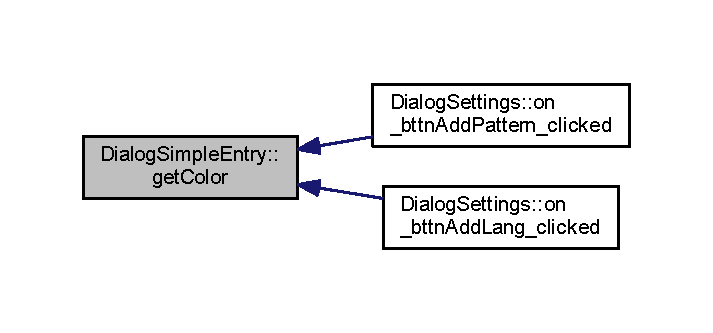
\includegraphics[width=342pt]{class_dialog_simple_entry_addf576d4bc4e1acbd27743c112f267b1_icgraph}
\end{center}
\end{figure}


\hypertarget{class_dialog_simple_entry_ab9f80cd88dae4100bfb47b9df2cd02ad}{\index{Dialog\+Simple\+Entry@{Dialog\+Simple\+Entry}!get\+Text\+Field\+Content@{get\+Text\+Field\+Content}}
\index{get\+Text\+Field\+Content@{get\+Text\+Field\+Content}!Dialog\+Simple\+Entry@{Dialog\+Simple\+Entry}}
\subsubsection[{get\+Text\+Field\+Content}]{\setlength{\rightskip}{0pt plus 5cm}Q\+String Dialog\+Simple\+Entry\+::get\+Text\+Field\+Content (
\begin{DoxyParamCaption}
{}
\end{DoxyParamCaption}
)}}\label{class_dialog_simple_entry_ab9f80cd88dae4100bfb47b9df2cd02ad}


\hyperlink{class_dialog_simple_entry_ab9f80cd88dae4100bfb47b9df2cd02ad}{Dialog\+Simple\+Entry\+::get\+Text\+Field\+Content}. 

Returns the content of the Q\+Line\+Edit.

\begin{DoxyReturn}{Returns}
content of the textfield 
\end{DoxyReturn}


Here is the caller graph for this function\+:
\nopagebreak
\begin{figure}[H]
\begin{center}
\leavevmode
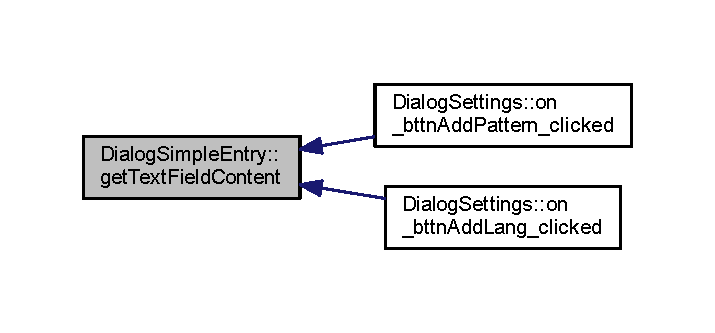
\includegraphics[width=343pt]{class_dialog_simple_entry_ab9f80cd88dae4100bfb47b9df2cd02ad_icgraph}
\end{center}
\end{figure}


\hypertarget{class_dialog_simple_entry_a08da9e5b778950ec6cf3172e04d5e4b4}{\index{Dialog\+Simple\+Entry@{Dialog\+Simple\+Entry}!on\+\_\+bttn\+Pick\+Color\+\_\+clicked@{on\+\_\+bttn\+Pick\+Color\+\_\+clicked}}
\index{on\+\_\+bttn\+Pick\+Color\+\_\+clicked@{on\+\_\+bttn\+Pick\+Color\+\_\+clicked}!Dialog\+Simple\+Entry@{Dialog\+Simple\+Entry}}
\subsubsection[{on\+\_\+bttn\+Pick\+Color\+\_\+clicked}]{\setlength{\rightskip}{0pt plus 5cm}void Dialog\+Simple\+Entry\+::on\+\_\+bttn\+Pick\+Color\+\_\+clicked (
\begin{DoxyParamCaption}
{}
\end{DoxyParamCaption}
)\hspace{0.3cm}{\ttfamily [private]}, {\ttfamily [slot]}}}\label{class_dialog_simple_entry_a08da9e5b778950ec6cf3172e04d5e4b4}


\hyperlink{class_dialog_simple_entry_a08da9e5b778950ec6cf3172e04d5e4b4}{Dialog\+Simple\+Entry\+::on\+\_\+bttn\+Pick\+Color\+\_\+clicked}. 

Opens up a Q\+Color\+Dialog and sets the background color of the Q\+Push\+Button to the selected color. 

\subsection{Member Data Documentation}
\hypertarget{class_dialog_simple_entry_a797fd737de17d712425cb61142a9789d}{\index{Dialog\+Simple\+Entry@{Dialog\+Simple\+Entry}!color@{color}}
\index{color@{color}!Dialog\+Simple\+Entry@{Dialog\+Simple\+Entry}}
\subsubsection[{color}]{\setlength{\rightskip}{0pt plus 5cm}Q\+Color Dialog\+Simple\+Entry\+::color\hspace{0.3cm}{\ttfamily [private]}}}\label{class_dialog_simple_entry_a797fd737de17d712425cb61142a9789d}
\hypertarget{class_dialog_simple_entry_a3ef78d511f3bd60f104be4851b8e8e7b}{\index{Dialog\+Simple\+Entry@{Dialog\+Simple\+Entry}!ui@{ui}}
\index{ui@{ui}!Dialog\+Simple\+Entry@{Dialog\+Simple\+Entry}}
\subsubsection[{ui}]{\setlength{\rightskip}{0pt plus 5cm}Ui\+::\+Dialog\+Simple\+Entry$\ast$ Dialog\+Simple\+Entry\+::ui\hspace{0.3cm}{\ttfamily [private]}}}\label{class_dialog_simple_entry_a3ef78d511f3bd60f104be4851b8e8e7b}


The documentation for this class was generated from the following files\+:\begin{DoxyCompactItemize}
\item 
D\+:/\+Entwicklung/\+C++/\+Workspace/\+Beleg\+Cpp/\hyperlink{dialogsimpleentry_8h}{dialogsimpleentry.\+h}\item 
D\+:/\+Entwicklung/\+C++/\+Workspace/\+Beleg\+Cpp/\hyperlink{dialogsimpleentry_8cpp}{dialogsimpleentry.\+cpp}\end{DoxyCompactItemize}

\hypertarget{class_entry_details}{\section{Entry\+Details Class Reference}
\label{class_entry_details}\index{Entry\+Details@{Entry\+Details}}
}


The \hyperlink{class_entry_details}{Entry\+Details} class.  




{\ttfamily \#include $<$entrydetails.\+h$>$}



Inheritance diagram for Entry\+Details\+:
\nopagebreak
\begin{figure}[H]
\begin{center}
\leavevmode
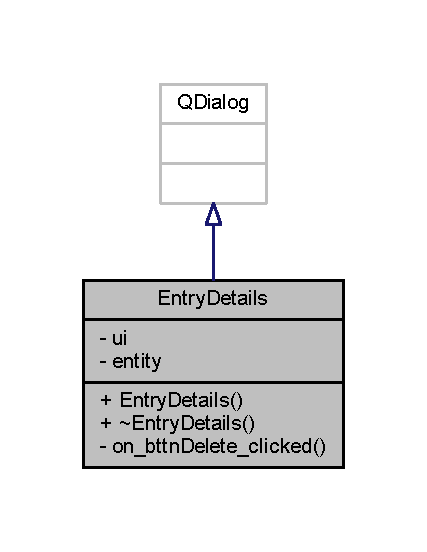
\includegraphics[width=205pt]{class_entry_details__inherit__graph}
\end{center}
\end{figure}


Collaboration diagram for Entry\+Details\+:
\nopagebreak
\begin{figure}[H]
\begin{center}
\leavevmode
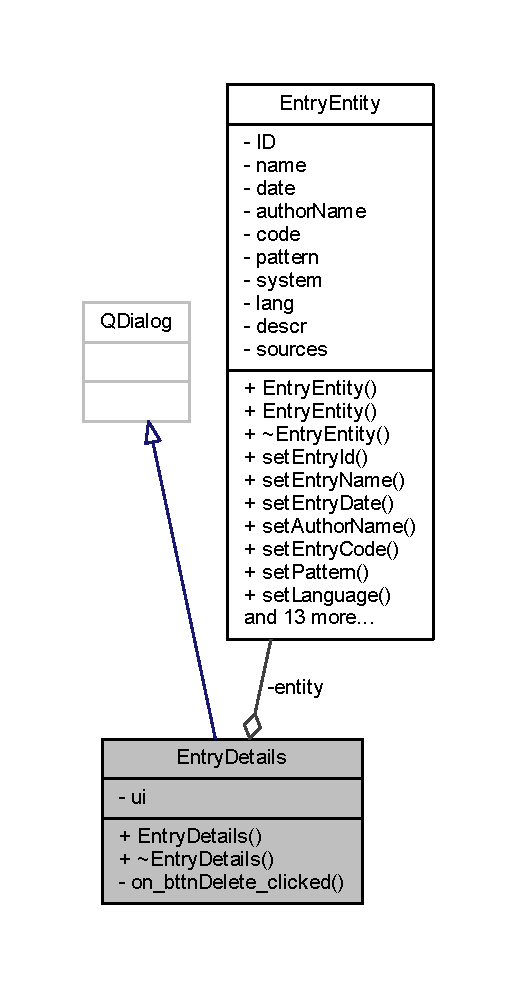
\includegraphics[width=248pt]{class_entry_details__coll__graph}
\end{center}
\end{figure}
\subsection*{Public Member Functions}
\begin{DoxyCompactItemize}
\item 
\hyperlink{class_entry_details_a636962c9912b8f6c25ed03ef10098423}{Entry\+Details} (\hyperlink{class_entry_entity}{Entry\+Entity} \hyperlink{class_entry_details_a8e6d1755f064f499cc5104aeb6985cb8}{entity}, Q\+Widget $\ast$parent=0)
\begin{DoxyCompactList}\small\item\em \hyperlink{class_entry_details_a636962c9912b8f6c25ed03ef10098423}{Entry\+Details\+::\+Entry\+Details}. \end{DoxyCompactList}\item 
\hyperlink{class_entry_details_ad500af502edaf2b661c7db036423699e}{$\sim$\+Entry\+Details} ()
\begin{DoxyCompactList}\small\item\em \hyperlink{class_entry_details_ad500af502edaf2b661c7db036423699e}{Entry\+Details\+::$\sim$\+Entry\+Details}. \end{DoxyCompactList}\end{DoxyCompactItemize}
\subsection*{Private Slots}
\begin{DoxyCompactItemize}
\item 
void \hyperlink{class_entry_details_a376e05a7c7299c3b292a16e994bd319b}{on\+\_\+bttn\+Delete\+\_\+clicked} ()
\begin{DoxyCompactList}\small\item\em \hyperlink{class_entry_details_a376e05a7c7299c3b292a16e994bd319b}{Entry\+Details\+::on\+\_\+bttn\+Delete\+\_\+clicked}. \end{DoxyCompactList}\end{DoxyCompactItemize}
\subsection*{Private Attributes}
\begin{DoxyCompactItemize}
\item 
Ui\+::\+Entry\+Details $\ast$ \hyperlink{class_entry_details_ae27c7423d1a1f3bee14af21371700db7}{ui}
\item 
\hyperlink{class_entry_entity}{Entry\+Entity} \hyperlink{class_entry_details_a8e6d1755f064f499cc5104aeb6985cb8}{entity}
\end{DoxyCompactItemize}


\subsection{Detailed Description}
The \hyperlink{class_entry_details}{Entry\+Details} class. 

This class represents a Q\+Dialog to show information about one entry.

\begin{DoxyAuthor}{Author}
Robert Wolfinger 
\end{DoxyAuthor}
\begin{DoxyVersion}{Version}
1.\+0 20.\+09.\+14 
\end{DoxyVersion}


\subsection{Constructor \& Destructor Documentation}
\hypertarget{class_entry_details_a636962c9912b8f6c25ed03ef10098423}{\index{Entry\+Details@{Entry\+Details}!Entry\+Details@{Entry\+Details}}
\index{Entry\+Details@{Entry\+Details}!Entry\+Details@{Entry\+Details}}
\subsubsection[{Entry\+Details}]{\setlength{\rightskip}{0pt plus 5cm}Entry\+Details\+::\+Entry\+Details (
\begin{DoxyParamCaption}
\item[{{\bf Entry\+Entity}}]{entity, }
\item[{Q\+Widget $\ast$}]{parent = {\ttfamily 0}}
\end{DoxyParamCaption}
)\hspace{0.3cm}{\ttfamily [explicit]}}}\label{class_entry_details_a636962c9912b8f6c25ed03ef10098423}


\hyperlink{class_entry_details_a636962c9912b8f6c25ed03ef10098423}{Entry\+Details\+::\+Entry\+Details}. 

\begin{DoxyAuthor}{Author}
Robert Wolfinger 
\end{DoxyAuthor}
\begin{DoxyVersion}{Version}
1.\+0 20.\+09.\+14 Constructs the dialog. All information is retrieved from the given \hyperlink{class_entry_entity}{Entry\+Entity} object and set as content of the appropriate labels.
\end{DoxyVersion}

\begin{DoxyParams}{Parameters}
{\em entity} & \\
\hline
{\em parent} & \\
\hline
\end{DoxyParams}


Here is the call graph for this function\+:\nopagebreak
\begin{figure}[H]
\begin{center}
\leavevmode
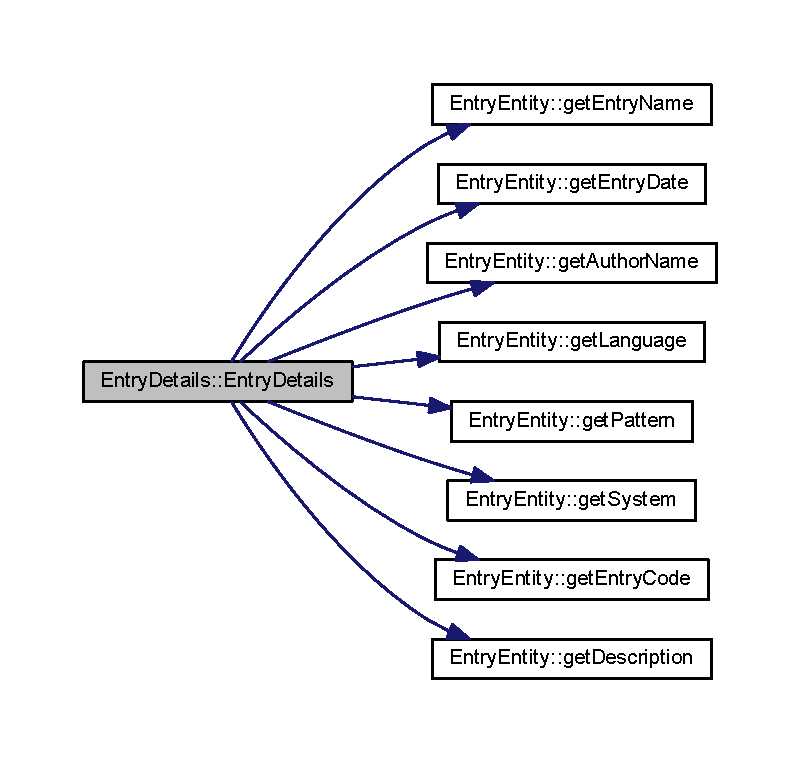
\includegraphics[width=350pt]{class_entry_details_a636962c9912b8f6c25ed03ef10098423_cgraph}
\end{center}
\end{figure}


\hypertarget{class_entry_details_ad500af502edaf2b661c7db036423699e}{\index{Entry\+Details@{Entry\+Details}!````~Entry\+Details@{$\sim$\+Entry\+Details}}
\index{````~Entry\+Details@{$\sim$\+Entry\+Details}!Entry\+Details@{Entry\+Details}}
\subsubsection[{$\sim$\+Entry\+Details}]{\setlength{\rightskip}{0pt plus 5cm}Entry\+Details\+::$\sim$\+Entry\+Details (
\begin{DoxyParamCaption}
{}
\end{DoxyParamCaption}
)}}\label{class_entry_details_ad500af502edaf2b661c7db036423699e}


\hyperlink{class_entry_details_ad500af502edaf2b661c7db036423699e}{Entry\+Details\+::$\sim$\+Entry\+Details}. 

Deconstructs the dialog. 

\subsection{Member Function Documentation}
\hypertarget{class_entry_details_a376e05a7c7299c3b292a16e994bd319b}{\index{Entry\+Details@{Entry\+Details}!on\+\_\+bttn\+Delete\+\_\+clicked@{on\+\_\+bttn\+Delete\+\_\+clicked}}
\index{on\+\_\+bttn\+Delete\+\_\+clicked@{on\+\_\+bttn\+Delete\+\_\+clicked}!Entry\+Details@{Entry\+Details}}
\subsubsection[{on\+\_\+bttn\+Delete\+\_\+clicked}]{\setlength{\rightskip}{0pt plus 5cm}void Entry\+Details\+::on\+\_\+bttn\+Delete\+\_\+clicked (
\begin{DoxyParamCaption}
{}
\end{DoxyParamCaption}
)\hspace{0.3cm}{\ttfamily [private]}, {\ttfamily [slot]}}}\label{class_entry_details_a376e05a7c7299c3b292a16e994bd319b}


\hyperlink{class_entry_details_a376e05a7c7299c3b292a16e994bd319b}{Entry\+Details\+::on\+\_\+bttn\+Delete\+\_\+clicked}. 

Deletes the entry in the database and closes the dialog. 

Here is the call graph for this function\+:
\nopagebreak
\begin{figure}[H]
\begin{center}
\leavevmode
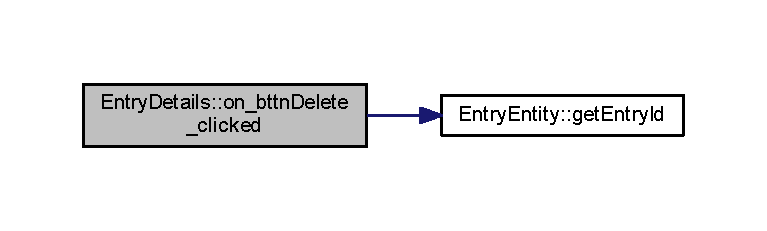
\includegraphics[width=350pt]{class_entry_details_a376e05a7c7299c3b292a16e994bd319b_cgraph}
\end{center}
\end{figure}




\subsection{Member Data Documentation}
\hypertarget{class_entry_details_a8e6d1755f064f499cc5104aeb6985cb8}{\index{Entry\+Details@{Entry\+Details}!entity@{entity}}
\index{entity@{entity}!Entry\+Details@{Entry\+Details}}
\subsubsection[{entity}]{\setlength{\rightskip}{0pt plus 5cm}{\bf Entry\+Entity} Entry\+Details\+::entity\hspace{0.3cm}{\ttfamily [private]}}}\label{class_entry_details_a8e6d1755f064f499cc5104aeb6985cb8}
\hypertarget{class_entry_details_ae27c7423d1a1f3bee14af21371700db7}{\index{Entry\+Details@{Entry\+Details}!ui@{ui}}
\index{ui@{ui}!Entry\+Details@{Entry\+Details}}
\subsubsection[{ui}]{\setlength{\rightskip}{0pt plus 5cm}Ui\+::\+Entry\+Details$\ast$ Entry\+Details\+::ui\hspace{0.3cm}{\ttfamily [private]}}}\label{class_entry_details_ae27c7423d1a1f3bee14af21371700db7}


The documentation for this class was generated from the following files\+:\begin{DoxyCompactItemize}
\item 
D\+:/\+Entwicklung/\+C++/\+Workspace/\+Beleg\+Cpp/\hyperlink{entrydetails_8h}{entrydetails.\+h}\item 
D\+:/\+Entwicklung/\+C++/\+Workspace/\+Beleg\+Cpp/\hyperlink{entrydetails_8cpp}{entrydetails.\+cpp}\end{DoxyCompactItemize}

\hypertarget{class_entry_entity}{\section{Entry\+Entity Class Reference}
\label{class_entry_entity}\index{Entry\+Entity@{Entry\+Entity}}
}


The \hyperlink{class_entry_entity}{Entry\+Entity} class.  




{\ttfamily \#include $<$entryentity.\+h$>$}



Collaboration diagram for Entry\+Entity\+:
\nopagebreak
\begin{figure}[H]
\begin{center}
\leavevmode
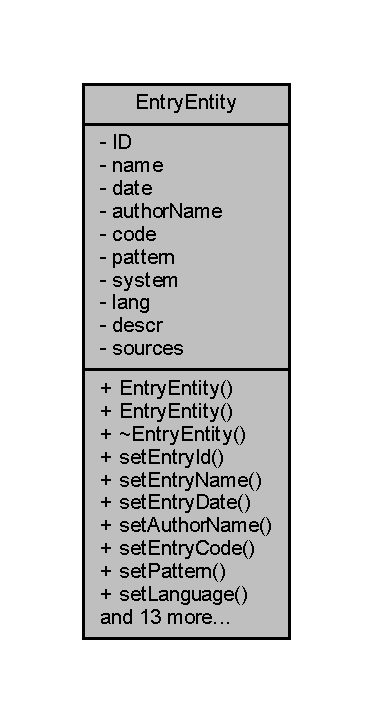
\includegraphics[width=179pt]{class_entry_entity__coll__graph}
\end{center}
\end{figure}
\subsection*{Public Member Functions}
\begin{DoxyCompactItemize}
\item 
\hyperlink{class_entry_entity_a4131db8f9e9a5f600948f32ec92b15a1}{Entry\+Entity} (int \hyperlink{class_entry_entity_a0353f8e056e80e3277f1cc6c17d2e071}{I\+D}, Q\+String entry\+Name, Q\+String entry\+Date, Q\+String \hyperlink{class_entry_entity_abeb114f6b0cfe1678a36e998e21434bf}{author\+Name}, Q\+String entry\+Code, Q\+String \hyperlink{class_entry_entity_a65f0a241d2a05f7b2da01e5868acfe5c}{pattern}, Q\+String \hyperlink{class_entry_entity_ab925c61d96e3e82745d185e931ef1e64}{system}, Q\+String \hyperlink{class_entry_entity_a5225b37537638e119ef901cad839390c}{lang}, Q\+String \hyperlink{class_entry_entity_ae87c35927889353ff5739e1fabe499bb}{descr}, int sources\+Key)
\begin{DoxyCompactList}\small\item\em \hyperlink{class_entry_entity_a4131db8f9e9a5f600948f32ec92b15a1}{Entry\+Entity\+::\+Entry\+Entity}. \end{DoxyCompactList}\item 
\hyperlink{class_entry_entity_a961e4826d03bfa25bfffbb67bd2fb659}{Entry\+Entity} ()
\begin{DoxyCompactList}\small\item\em \hyperlink{class_entry_entity_a4131db8f9e9a5f600948f32ec92b15a1}{Entry\+Entity\+::\+Entry\+Entity}. \end{DoxyCompactList}\item 
\hyperlink{class_entry_entity_a1f6cbe666bbaea1653ece144559fea36}{$\sim$\+Entry\+Entity} ()
\begin{DoxyCompactList}\small\item\em \hyperlink{class_entry_entity_a1f6cbe666bbaea1653ece144559fea36}{Entry\+Entity\+::$\sim$\+Entry\+Entity}. \end{DoxyCompactList}\item 
void \hyperlink{class_entry_entity_a64412ce49af6eee9c1d9ff5a884f9127}{set\+Entry\+Id} (int id)
\item 
void \hyperlink{class_entry_entity_a96b5fdfb05183a9c8f570abb3c73e974}{set\+Entry\+Name} (Q\+String entry\+Name)
\item 
void \hyperlink{class_entry_entity_a20c8ff5f7b29bc6a54a68fde6318f365}{set\+Entry\+Date} (Q\+String entry\+Date)
\item 
void \hyperlink{class_entry_entity_ae99e4feb875823e643b62c0f9b0a2771}{set\+Author\+Name} (Q\+String \hyperlink{class_entry_entity_abeb114f6b0cfe1678a36e998e21434bf}{author\+Name})
\item 
void \hyperlink{class_entry_entity_a705759132ac39477ace6b35a431ac5f6}{set\+Entry\+Code} (Q\+String entry\+Code)
\item 
void \hyperlink{class_entry_entity_a255b536a9474e681bf5023f55188a1c6}{set\+Pattern} (Q\+String \hyperlink{class_entry_entity_a65f0a241d2a05f7b2da01e5868acfe5c}{pattern})
\item 
void \hyperlink{class_entry_entity_a0a4e25af4be8c937f2dcdcfb054b5d49}{set\+Language} (Q\+String language)
\item 
void \hyperlink{class_entry_entity_aa99b5179f72cdc9aebcae8618402dde9}{set\+System} (Q\+String \hyperlink{class_entry_entity_ab925c61d96e3e82745d185e931ef1e64}{system})
\item 
void \hyperlink{class_entry_entity_a814f4b55969c9da7785cf299e450f6a1}{set\+Description} (Q\+String description)
\item 
void \hyperlink{class_entry_entity_a55b1678e5b67b722c0b76a54b85061d3}{set\+Source\+Key} (int key)
\item 
int \hyperlink{class_entry_entity_a6153d3a94a44c9774e39f0ae0de2e0ad}{get\+Entry\+Id} ()
\item 
Q\+String \hyperlink{class_entry_entity_a1f07642efaed25e9725ed130258c4f3f}{get\+Entry\+Name} ()
\item 
Q\+String \hyperlink{class_entry_entity_a3f1c1dd15ed91ce6215d6e44dd3b2be7}{get\+Entry\+Date} ()
\item 
Q\+String \hyperlink{class_entry_entity_a0cfdd408fe4a6daf0f859c1fbb2b0773}{get\+Author\+Name} ()
\item 
Q\+String \hyperlink{class_entry_entity_a0f6a2ead8b72da01c9b5461e3b0ceac2}{get\+Entry\+Code} ()
\item 
Q\+String \hyperlink{class_entry_entity_a8386a3a73fbd18e2c567ab93db643e2b}{get\+Pattern} ()
\item 
Q\+String \hyperlink{class_entry_entity_a90856a316a8dc5ccb78236ad8399dbb9}{get\+System} ()
\item 
Q\+String \hyperlink{class_entry_entity_a8d72297bafb99e6e6761f8b9f32888ef}{get\+Language} ()
\item 
Q\+String \hyperlink{class_entry_entity_a7636ecdfd90c39b1548264d5be9bc05d}{get\+Description} ()
\item 
int \hyperlink{class_entry_entity_a4cd1f6dfc7c40981239415b265fe32c1}{get\+Source\+Key} ()
\end{DoxyCompactItemize}
\subsection*{Private Attributes}
\begin{DoxyCompactItemize}
\item 
int \hyperlink{class_entry_entity_a0353f8e056e80e3277f1cc6c17d2e071}{I\+D}
\item 
Q\+String \hyperlink{class_entry_entity_aa56cd8b59742ac7970d5344b93ae88a0}{name}
\item 
Q\+String \hyperlink{class_entry_entity_ad5ebe98873fec2e521b5df2b31a4b7b6}{date}
\item 
Q\+String \hyperlink{class_entry_entity_abeb114f6b0cfe1678a36e998e21434bf}{author\+Name}
\item 
Q\+String \hyperlink{class_entry_entity_a12393012ebcfc513af6eda5d95d9ccdb}{code}
\item 
Q\+String \hyperlink{class_entry_entity_a65f0a241d2a05f7b2da01e5868acfe5c}{pattern}
\item 
Q\+String \hyperlink{class_entry_entity_ab925c61d96e3e82745d185e931ef1e64}{system}
\item 
Q\+String \hyperlink{class_entry_entity_a5225b37537638e119ef901cad839390c}{lang}
\item 
Q\+String \hyperlink{class_entry_entity_ae87c35927889353ff5739e1fabe499bb}{descr}
\item 
int \hyperlink{class_entry_entity_af12b80bb0722b8a8d596f23289b5228a}{sources}
\end{DoxyCompactItemize}


\subsection{Detailed Description}
The \hyperlink{class_entry_entity}{Entry\+Entity} class. 

This class is used to represent the entry table in the database.

\begin{DoxyAuthor}{Author}
Robert Wolfinger 
\end{DoxyAuthor}
\begin{DoxyVersion}{Version}
1.\+0 20.\+09.\+14 
\end{DoxyVersion}


\subsection{Constructor \& Destructor Documentation}
\hypertarget{class_entry_entity_a4131db8f9e9a5f600948f32ec92b15a1}{\index{Entry\+Entity@{Entry\+Entity}!Entry\+Entity@{Entry\+Entity}}
\index{Entry\+Entity@{Entry\+Entity}!Entry\+Entity@{Entry\+Entity}}
\subsubsection[{Entry\+Entity}]{\setlength{\rightskip}{0pt plus 5cm}Entry\+Entity\+::\+Entry\+Entity (
\begin{DoxyParamCaption}
\item[{int}]{I\+D, }
\item[{Q\+String}]{entry\+Name, }
\item[{Q\+String}]{entry\+Date, }
\item[{Q\+String}]{author\+Name, }
\item[{Q\+String}]{entry\+Code, }
\item[{Q\+String}]{pattern, }
\item[{Q\+String}]{system, }
\item[{Q\+String}]{lang, }
\item[{Q\+String}]{descr, }
\item[{int}]{sources\+Key}
\end{DoxyParamCaption}
)}}\label{class_entry_entity_a4131db8f9e9a5f600948f32ec92b15a1}


\hyperlink{class_entry_entity_a4131db8f9e9a5f600948f32ec92b15a1}{Entry\+Entity\+::\+Entry\+Entity}. 

Constructor for an entry.


\begin{DoxyParams}{Parameters}
{\em I\+D} & \\
\hline
{\em entry\+Name} & \\
\hline
{\em entry\+Date} & \\
\hline
{\em author\+Name} & \\
\hline
{\em entry\+Code} & \\
\hline
{\em pattern} & \\
\hline
{\em system} & \\
\hline
{\em lang} & \\
\hline
{\em descr} & \\
\hline
{\em sources\+Key} & \\
\hline
\end{DoxyParams}


Here is the call graph for this function\+:\nopagebreak
\begin{figure}[H]
\begin{center}
\leavevmode
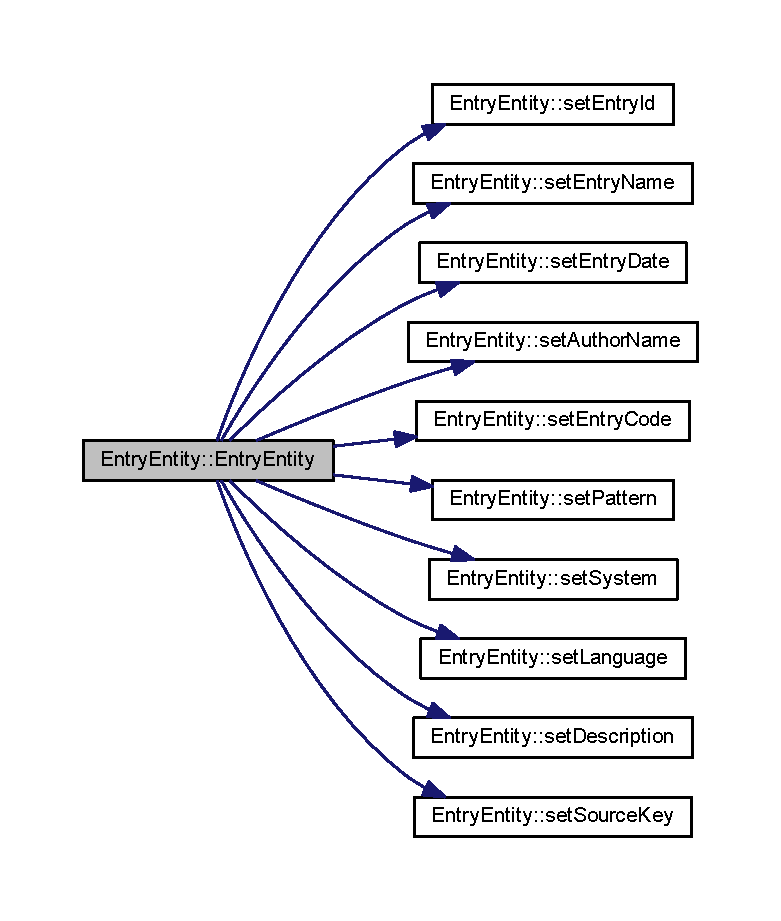
\includegraphics[width=350pt]{class_entry_entity_a4131db8f9e9a5f600948f32ec92b15a1_cgraph}
\end{center}
\end{figure}


\hypertarget{class_entry_entity_a961e4826d03bfa25bfffbb67bd2fb659}{\index{Entry\+Entity@{Entry\+Entity}!Entry\+Entity@{Entry\+Entity}}
\index{Entry\+Entity@{Entry\+Entity}!Entry\+Entity@{Entry\+Entity}}
\subsubsection[{Entry\+Entity}]{\setlength{\rightskip}{0pt plus 5cm}Entry\+Entity\+::\+Entry\+Entity (
\begin{DoxyParamCaption}
{}
\end{DoxyParamCaption}
)}}\label{class_entry_entity_a961e4826d03bfa25bfffbb67bd2fb659}


\hyperlink{class_entry_entity_a4131db8f9e9a5f600948f32ec92b15a1}{Entry\+Entity\+::\+Entry\+Entity}. 

\begin{DoxyAuthor}{Author}
Robert Wolfinger 
\end{DoxyAuthor}
\begin{DoxyVersion}{Version}
1.\+0 20.\+09.\+14 Constructor for an empty entry. 
\end{DoxyVersion}


Here is the call graph for this function\+:\nopagebreak
\begin{figure}[H]
\begin{center}
\leavevmode
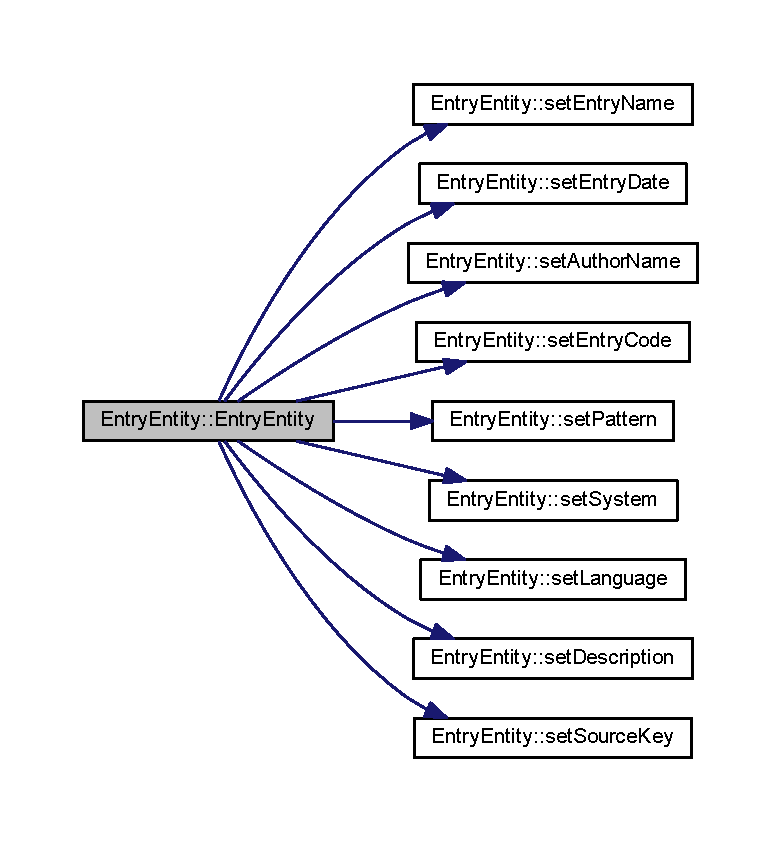
\includegraphics[width=350pt]{class_entry_entity_a961e4826d03bfa25bfffbb67bd2fb659_cgraph}
\end{center}
\end{figure}


\hypertarget{class_entry_entity_a1f6cbe666bbaea1653ece144559fea36}{\index{Entry\+Entity@{Entry\+Entity}!````~Entry\+Entity@{$\sim$\+Entry\+Entity}}
\index{````~Entry\+Entity@{$\sim$\+Entry\+Entity}!Entry\+Entity@{Entry\+Entity}}
\subsubsection[{$\sim$\+Entry\+Entity}]{\setlength{\rightskip}{0pt plus 5cm}Entry\+Entity\+::$\sim$\+Entry\+Entity (
\begin{DoxyParamCaption}
{}
\end{DoxyParamCaption}
)}}\label{class_entry_entity_a1f6cbe666bbaea1653ece144559fea36}


\hyperlink{class_entry_entity_a1f6cbe666bbaea1653ece144559fea36}{Entry\+Entity\+::$\sim$\+Entry\+Entity}. 

Deconstructor for the entity object. 

\subsection{Member Function Documentation}
\hypertarget{class_entry_entity_a0cfdd408fe4a6daf0f859c1fbb2b0773}{\index{Entry\+Entity@{Entry\+Entity}!get\+Author\+Name@{get\+Author\+Name}}
\index{get\+Author\+Name@{get\+Author\+Name}!Entry\+Entity@{Entry\+Entity}}
\subsubsection[{get\+Author\+Name}]{\setlength{\rightskip}{0pt plus 5cm}Q\+String Entry\+Entity\+::get\+Author\+Name (
\begin{DoxyParamCaption}
{}
\end{DoxyParamCaption}
)}}\label{class_entry_entity_a0cfdd408fe4a6daf0f859c1fbb2b0773}


Here is the caller graph for this function\+:\nopagebreak
\begin{figure}[H]
\begin{center}
\leavevmode
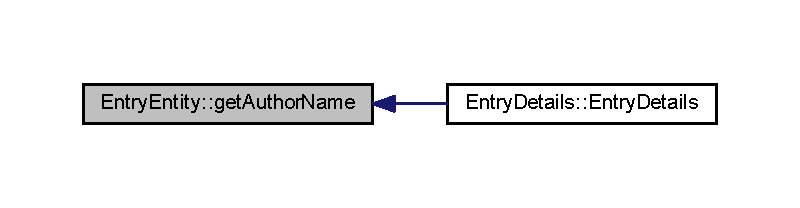
\includegraphics[width=350pt]{class_entry_entity_a0cfdd408fe4a6daf0f859c1fbb2b0773_icgraph}
\end{center}
\end{figure}


\hypertarget{class_entry_entity_a7636ecdfd90c39b1548264d5be9bc05d}{\index{Entry\+Entity@{Entry\+Entity}!get\+Description@{get\+Description}}
\index{get\+Description@{get\+Description}!Entry\+Entity@{Entry\+Entity}}
\subsubsection[{get\+Description}]{\setlength{\rightskip}{0pt plus 5cm}Q\+String Entry\+Entity\+::get\+Description (
\begin{DoxyParamCaption}
{}
\end{DoxyParamCaption}
)}}\label{class_entry_entity_a7636ecdfd90c39b1548264d5be9bc05d}


Here is the caller graph for this function\+:\nopagebreak
\begin{figure}[H]
\begin{center}
\leavevmode
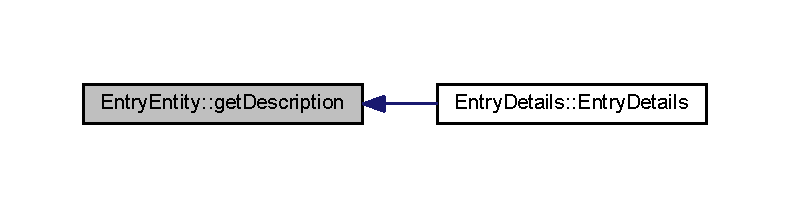
\includegraphics[width=350pt]{class_entry_entity_a7636ecdfd90c39b1548264d5be9bc05d_icgraph}
\end{center}
\end{figure}


\hypertarget{class_entry_entity_a0f6a2ead8b72da01c9b5461e3b0ceac2}{\index{Entry\+Entity@{Entry\+Entity}!get\+Entry\+Code@{get\+Entry\+Code}}
\index{get\+Entry\+Code@{get\+Entry\+Code}!Entry\+Entity@{Entry\+Entity}}
\subsubsection[{get\+Entry\+Code}]{\setlength{\rightskip}{0pt plus 5cm}Q\+String Entry\+Entity\+::get\+Entry\+Code (
\begin{DoxyParamCaption}
{}
\end{DoxyParamCaption}
)}}\label{class_entry_entity_a0f6a2ead8b72da01c9b5461e3b0ceac2}


Here is the caller graph for this function\+:\nopagebreak
\begin{figure}[H]
\begin{center}
\leavevmode
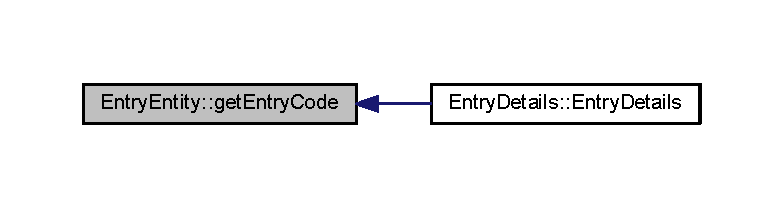
\includegraphics[width=350pt]{class_entry_entity_a0f6a2ead8b72da01c9b5461e3b0ceac2_icgraph}
\end{center}
\end{figure}


\hypertarget{class_entry_entity_a3f1c1dd15ed91ce6215d6e44dd3b2be7}{\index{Entry\+Entity@{Entry\+Entity}!get\+Entry\+Date@{get\+Entry\+Date}}
\index{get\+Entry\+Date@{get\+Entry\+Date}!Entry\+Entity@{Entry\+Entity}}
\subsubsection[{get\+Entry\+Date}]{\setlength{\rightskip}{0pt plus 5cm}Q\+String Entry\+Entity\+::get\+Entry\+Date (
\begin{DoxyParamCaption}
{}
\end{DoxyParamCaption}
)}}\label{class_entry_entity_a3f1c1dd15ed91ce6215d6e44dd3b2be7}


Here is the caller graph for this function\+:\nopagebreak
\begin{figure}[H]
\begin{center}
\leavevmode
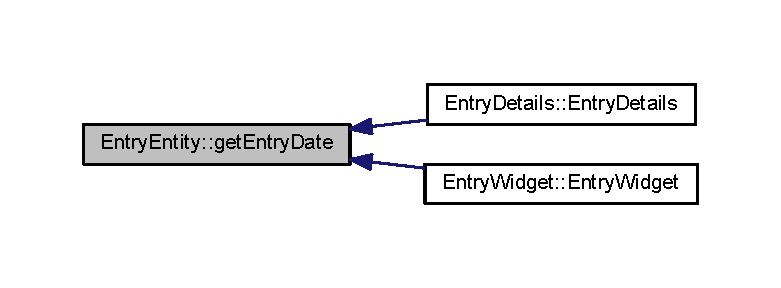
\includegraphics[width=350pt]{class_entry_entity_a3f1c1dd15ed91ce6215d6e44dd3b2be7_icgraph}
\end{center}
\end{figure}


\hypertarget{class_entry_entity_a6153d3a94a44c9774e39f0ae0de2e0ad}{\index{Entry\+Entity@{Entry\+Entity}!get\+Entry\+Id@{get\+Entry\+Id}}
\index{get\+Entry\+Id@{get\+Entry\+Id}!Entry\+Entity@{Entry\+Entity}}
\subsubsection[{get\+Entry\+Id}]{\setlength{\rightskip}{0pt plus 5cm}int Entry\+Entity\+::get\+Entry\+Id (
\begin{DoxyParamCaption}
{}
\end{DoxyParamCaption}
)}}\label{class_entry_entity_a6153d3a94a44c9774e39f0ae0de2e0ad}


Here is the caller graph for this function\+:
\nopagebreak
\begin{figure}[H]
\begin{center}
\leavevmode
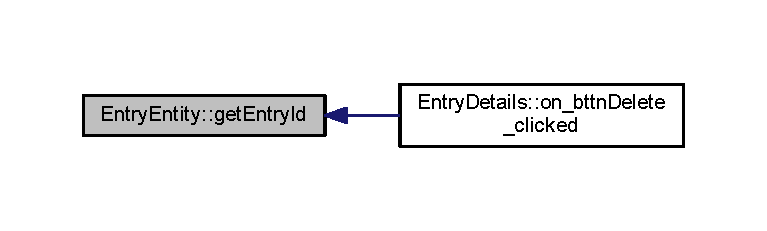
\includegraphics[width=350pt]{class_entry_entity_a6153d3a94a44c9774e39f0ae0de2e0ad_icgraph}
\end{center}
\end{figure}


\hypertarget{class_entry_entity_a1f07642efaed25e9725ed130258c4f3f}{\index{Entry\+Entity@{Entry\+Entity}!get\+Entry\+Name@{get\+Entry\+Name}}
\index{get\+Entry\+Name@{get\+Entry\+Name}!Entry\+Entity@{Entry\+Entity}}
\subsubsection[{get\+Entry\+Name}]{\setlength{\rightskip}{0pt plus 5cm}Q\+String Entry\+Entity\+::get\+Entry\+Name (
\begin{DoxyParamCaption}
{}
\end{DoxyParamCaption}
)}}\label{class_entry_entity_a1f07642efaed25e9725ed130258c4f3f}


Here is the caller graph for this function\+:\nopagebreak
\begin{figure}[H]
\begin{center}
\leavevmode
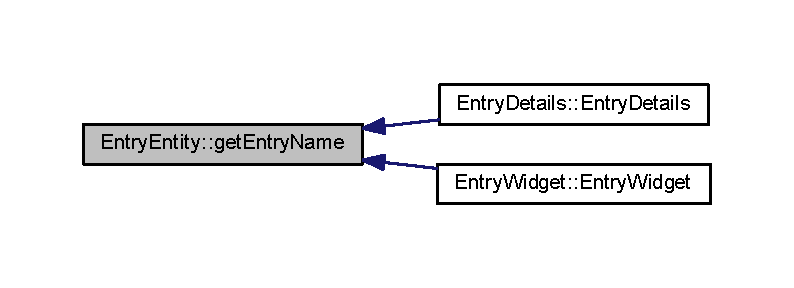
\includegraphics[width=350pt]{class_entry_entity_a1f07642efaed25e9725ed130258c4f3f_icgraph}
\end{center}
\end{figure}


\hypertarget{class_entry_entity_a8d72297bafb99e6e6761f8b9f32888ef}{\index{Entry\+Entity@{Entry\+Entity}!get\+Language@{get\+Language}}
\index{get\+Language@{get\+Language}!Entry\+Entity@{Entry\+Entity}}
\subsubsection[{get\+Language}]{\setlength{\rightskip}{0pt plus 5cm}Q\+String Entry\+Entity\+::get\+Language (
\begin{DoxyParamCaption}
{}
\end{DoxyParamCaption}
)}}\label{class_entry_entity_a8d72297bafb99e6e6761f8b9f32888ef}


Here is the caller graph for this function\+:
\nopagebreak
\begin{figure}[H]
\begin{center}
\leavevmode
\includegraphics[width=350pt]{class_entry_entity_a8d72297bafb99e6e6761f8b9f32888ef_icgraph}
\end{center}
\end{figure}


\hypertarget{class_entry_entity_a8386a3a73fbd18e2c567ab93db643e2b}{\index{Entry\+Entity@{Entry\+Entity}!get\+Pattern@{get\+Pattern}}
\index{get\+Pattern@{get\+Pattern}!Entry\+Entity@{Entry\+Entity}}
\subsubsection[{get\+Pattern}]{\setlength{\rightskip}{0pt plus 5cm}Q\+String Entry\+Entity\+::get\+Pattern (
\begin{DoxyParamCaption}
{}
\end{DoxyParamCaption}
)}}\label{class_entry_entity_a8386a3a73fbd18e2c567ab93db643e2b}


Here is the caller graph for this function\+:
\nopagebreak
\begin{figure}[H]
\begin{center}
\leavevmode
\includegraphics[width=350pt]{class_entry_entity_a8386a3a73fbd18e2c567ab93db643e2b_icgraph}
\end{center}
\end{figure}


\hypertarget{class_entry_entity_a4cd1f6dfc7c40981239415b265fe32c1}{\index{Entry\+Entity@{Entry\+Entity}!get\+Source\+Key@{get\+Source\+Key}}
\index{get\+Source\+Key@{get\+Source\+Key}!Entry\+Entity@{Entry\+Entity}}
\subsubsection[{get\+Source\+Key}]{\setlength{\rightskip}{0pt plus 5cm}int Entry\+Entity\+::get\+Source\+Key (
\begin{DoxyParamCaption}
{}
\end{DoxyParamCaption}
)}}\label{class_entry_entity_a4cd1f6dfc7c40981239415b265fe32c1}
\hypertarget{class_entry_entity_a90856a316a8dc5ccb78236ad8399dbb9}{\index{Entry\+Entity@{Entry\+Entity}!get\+System@{get\+System}}
\index{get\+System@{get\+System}!Entry\+Entity@{Entry\+Entity}}
\subsubsection[{get\+System}]{\setlength{\rightskip}{0pt plus 5cm}Q\+String Entry\+Entity\+::get\+System (
\begin{DoxyParamCaption}
{}
\end{DoxyParamCaption}
)}}\label{class_entry_entity_a90856a316a8dc5ccb78236ad8399dbb9}


Here is the caller graph for this function\+:\nopagebreak
\begin{figure}[H]
\begin{center}
\leavevmode
\includegraphics[width=350pt]{class_entry_entity_a90856a316a8dc5ccb78236ad8399dbb9_icgraph}
\end{center}
\end{figure}


\hypertarget{class_entry_entity_ae99e4feb875823e643b62c0f9b0a2771}{\index{Entry\+Entity@{Entry\+Entity}!set\+Author\+Name@{set\+Author\+Name}}
\index{set\+Author\+Name@{set\+Author\+Name}!Entry\+Entity@{Entry\+Entity}}
\subsubsection[{set\+Author\+Name}]{\setlength{\rightskip}{0pt plus 5cm}void Entry\+Entity\+::set\+Author\+Name (
\begin{DoxyParamCaption}
\item[{Q\+String}]{author\+Name}
\end{DoxyParamCaption}
)}}\label{class_entry_entity_ae99e4feb875823e643b62c0f9b0a2771}


Here is the caller graph for this function\+:
\nopagebreak
\begin{figure}[H]
\begin{center}
\leavevmode
\includegraphics[width=350pt]{class_entry_entity_ae99e4feb875823e643b62c0f9b0a2771_icgraph}
\end{center}
\end{figure}


\hypertarget{class_entry_entity_a814f4b55969c9da7785cf299e450f6a1}{\index{Entry\+Entity@{Entry\+Entity}!set\+Description@{set\+Description}}
\index{set\+Description@{set\+Description}!Entry\+Entity@{Entry\+Entity}}
\subsubsection[{set\+Description}]{\setlength{\rightskip}{0pt plus 5cm}void Entry\+Entity\+::set\+Description (
\begin{DoxyParamCaption}
\item[{Q\+String}]{description}
\end{DoxyParamCaption}
)}}\label{class_entry_entity_a814f4b55969c9da7785cf299e450f6a1}


Here is the caller graph for this function\+:
\nopagebreak
\begin{figure}[H]
\begin{center}
\leavevmode
\includegraphics[width=350pt]{class_entry_entity_a814f4b55969c9da7785cf299e450f6a1_icgraph}
\end{center}
\end{figure}


\hypertarget{class_entry_entity_a705759132ac39477ace6b35a431ac5f6}{\index{Entry\+Entity@{Entry\+Entity}!set\+Entry\+Code@{set\+Entry\+Code}}
\index{set\+Entry\+Code@{set\+Entry\+Code}!Entry\+Entity@{Entry\+Entity}}
\subsubsection[{set\+Entry\+Code}]{\setlength{\rightskip}{0pt plus 5cm}void Entry\+Entity\+::set\+Entry\+Code (
\begin{DoxyParamCaption}
\item[{Q\+String}]{entry\+Code}
\end{DoxyParamCaption}
)}}\label{class_entry_entity_a705759132ac39477ace6b35a431ac5f6}


Here is the caller graph for this function\+:
\nopagebreak
\begin{figure}[H]
\begin{center}
\leavevmode
\includegraphics[width=350pt]{class_entry_entity_a705759132ac39477ace6b35a431ac5f6_icgraph}
\end{center}
\end{figure}


\hypertarget{class_entry_entity_a20c8ff5f7b29bc6a54a68fde6318f365}{\index{Entry\+Entity@{Entry\+Entity}!set\+Entry\+Date@{set\+Entry\+Date}}
\index{set\+Entry\+Date@{set\+Entry\+Date}!Entry\+Entity@{Entry\+Entity}}
\subsubsection[{set\+Entry\+Date}]{\setlength{\rightskip}{0pt plus 5cm}void Entry\+Entity\+::set\+Entry\+Date (
\begin{DoxyParamCaption}
\item[{Q\+String}]{entry\+Date}
\end{DoxyParamCaption}
)}}\label{class_entry_entity_a20c8ff5f7b29bc6a54a68fde6318f365}


Here is the caller graph for this function\+:
\nopagebreak
\begin{figure}[H]
\begin{center}
\leavevmode
\includegraphics[width=350pt]{class_entry_entity_a20c8ff5f7b29bc6a54a68fde6318f365_icgraph}
\end{center}
\end{figure}


\hypertarget{class_entry_entity_a64412ce49af6eee9c1d9ff5a884f9127}{\index{Entry\+Entity@{Entry\+Entity}!set\+Entry\+Id@{set\+Entry\+Id}}
\index{set\+Entry\+Id@{set\+Entry\+Id}!Entry\+Entity@{Entry\+Entity}}
\subsubsection[{set\+Entry\+Id}]{\setlength{\rightskip}{0pt plus 5cm}void Entry\+Entity\+::set\+Entry\+Id (
\begin{DoxyParamCaption}
\item[{int}]{id}
\end{DoxyParamCaption}
)}}\label{class_entry_entity_a64412ce49af6eee9c1d9ff5a884f9127}


Here is the caller graph for this function\+:
\nopagebreak
\begin{figure}[H]
\begin{center}
\leavevmode
\includegraphics[width=350pt]{class_entry_entity_a64412ce49af6eee9c1d9ff5a884f9127_icgraph}
\end{center}
\end{figure}


\hypertarget{class_entry_entity_a96b5fdfb05183a9c8f570abb3c73e974}{\index{Entry\+Entity@{Entry\+Entity}!set\+Entry\+Name@{set\+Entry\+Name}}
\index{set\+Entry\+Name@{set\+Entry\+Name}!Entry\+Entity@{Entry\+Entity}}
\subsubsection[{set\+Entry\+Name}]{\setlength{\rightskip}{0pt plus 5cm}void Entry\+Entity\+::set\+Entry\+Name (
\begin{DoxyParamCaption}
\item[{Q\+String}]{entry\+Name}
\end{DoxyParamCaption}
)}}\label{class_entry_entity_a96b5fdfb05183a9c8f570abb3c73e974}


Here is the caller graph for this function\+:
\nopagebreak
\begin{figure}[H]
\begin{center}
\leavevmode
\includegraphics[width=350pt]{class_entry_entity_a96b5fdfb05183a9c8f570abb3c73e974_icgraph}
\end{center}
\end{figure}


\hypertarget{class_entry_entity_a0a4e25af4be8c937f2dcdcfb054b5d49}{\index{Entry\+Entity@{Entry\+Entity}!set\+Language@{set\+Language}}
\index{set\+Language@{set\+Language}!Entry\+Entity@{Entry\+Entity}}
\subsubsection[{set\+Language}]{\setlength{\rightskip}{0pt plus 5cm}void Entry\+Entity\+::set\+Language (
\begin{DoxyParamCaption}
\item[{Q\+String}]{language}
\end{DoxyParamCaption}
)}}\label{class_entry_entity_a0a4e25af4be8c937f2dcdcfb054b5d49}


Here is the caller graph for this function\+:
\nopagebreak
\begin{figure}[H]
\begin{center}
\leavevmode
\includegraphics[width=350pt]{class_entry_entity_a0a4e25af4be8c937f2dcdcfb054b5d49_icgraph}
\end{center}
\end{figure}


\hypertarget{class_entry_entity_a255b536a9474e681bf5023f55188a1c6}{\index{Entry\+Entity@{Entry\+Entity}!set\+Pattern@{set\+Pattern}}
\index{set\+Pattern@{set\+Pattern}!Entry\+Entity@{Entry\+Entity}}
\subsubsection[{set\+Pattern}]{\setlength{\rightskip}{0pt plus 5cm}void Entry\+Entity\+::set\+Pattern (
\begin{DoxyParamCaption}
\item[{Q\+String}]{pattern}
\end{DoxyParamCaption}
)}}\label{class_entry_entity_a255b536a9474e681bf5023f55188a1c6}


Here is the caller graph for this function\+:
\nopagebreak
\begin{figure}[H]
\begin{center}
\leavevmode
\includegraphics[width=350pt]{class_entry_entity_a255b536a9474e681bf5023f55188a1c6_icgraph}
\end{center}
\end{figure}


\hypertarget{class_entry_entity_a55b1678e5b67b722c0b76a54b85061d3}{\index{Entry\+Entity@{Entry\+Entity}!set\+Source\+Key@{set\+Source\+Key}}
\index{set\+Source\+Key@{set\+Source\+Key}!Entry\+Entity@{Entry\+Entity}}
\subsubsection[{set\+Source\+Key}]{\setlength{\rightskip}{0pt plus 5cm}void Entry\+Entity\+::set\+Source\+Key (
\begin{DoxyParamCaption}
\item[{int}]{key}
\end{DoxyParamCaption}
)}}\label{class_entry_entity_a55b1678e5b67b722c0b76a54b85061d3}


Here is the caller graph for this function\+:
\nopagebreak
\begin{figure}[H]
\begin{center}
\leavevmode
\includegraphics[width=350pt]{class_entry_entity_a55b1678e5b67b722c0b76a54b85061d3_icgraph}
\end{center}
\end{figure}


\hypertarget{class_entry_entity_aa99b5179f72cdc9aebcae8618402dde9}{\index{Entry\+Entity@{Entry\+Entity}!set\+System@{set\+System}}
\index{set\+System@{set\+System}!Entry\+Entity@{Entry\+Entity}}
\subsubsection[{set\+System}]{\setlength{\rightskip}{0pt plus 5cm}void Entry\+Entity\+::set\+System (
\begin{DoxyParamCaption}
\item[{Q\+String}]{system}
\end{DoxyParamCaption}
)}}\label{class_entry_entity_aa99b5179f72cdc9aebcae8618402dde9}


Here is the caller graph for this function\+:
\nopagebreak
\begin{figure}[H]
\begin{center}
\leavevmode
\includegraphics[width=350pt]{class_entry_entity_aa99b5179f72cdc9aebcae8618402dde9_icgraph}
\end{center}
\end{figure}




\subsection{Member Data Documentation}
\hypertarget{class_entry_entity_abeb114f6b0cfe1678a36e998e21434bf}{\index{Entry\+Entity@{Entry\+Entity}!author\+Name@{author\+Name}}
\index{author\+Name@{author\+Name}!Entry\+Entity@{Entry\+Entity}}
\subsubsection[{author\+Name}]{\setlength{\rightskip}{0pt plus 5cm}Q\+String Entry\+Entity\+::author\+Name\hspace{0.3cm}{\ttfamily [private]}}}\label{class_entry_entity_abeb114f6b0cfe1678a36e998e21434bf}
\hypertarget{class_entry_entity_a12393012ebcfc513af6eda5d95d9ccdb}{\index{Entry\+Entity@{Entry\+Entity}!code@{code}}
\index{code@{code}!Entry\+Entity@{Entry\+Entity}}
\subsubsection[{code}]{\setlength{\rightskip}{0pt plus 5cm}Q\+String Entry\+Entity\+::code\hspace{0.3cm}{\ttfamily [private]}}}\label{class_entry_entity_a12393012ebcfc513af6eda5d95d9ccdb}
\hypertarget{class_entry_entity_ad5ebe98873fec2e521b5df2b31a4b7b6}{\index{Entry\+Entity@{Entry\+Entity}!date@{date}}
\index{date@{date}!Entry\+Entity@{Entry\+Entity}}
\subsubsection[{date}]{\setlength{\rightskip}{0pt plus 5cm}Q\+String Entry\+Entity\+::date\hspace{0.3cm}{\ttfamily [private]}}}\label{class_entry_entity_ad5ebe98873fec2e521b5df2b31a4b7b6}
\hypertarget{class_entry_entity_ae87c35927889353ff5739e1fabe499bb}{\index{Entry\+Entity@{Entry\+Entity}!descr@{descr}}
\index{descr@{descr}!Entry\+Entity@{Entry\+Entity}}
\subsubsection[{descr}]{\setlength{\rightskip}{0pt plus 5cm}Q\+String Entry\+Entity\+::descr\hspace{0.3cm}{\ttfamily [private]}}}\label{class_entry_entity_ae87c35927889353ff5739e1fabe499bb}
\hypertarget{class_entry_entity_a0353f8e056e80e3277f1cc6c17d2e071}{\index{Entry\+Entity@{Entry\+Entity}!I\+D@{I\+D}}
\index{I\+D@{I\+D}!Entry\+Entity@{Entry\+Entity}}
\subsubsection[{I\+D}]{\setlength{\rightskip}{0pt plus 5cm}int Entry\+Entity\+::\+I\+D\hspace{0.3cm}{\ttfamily [private]}}}\label{class_entry_entity_a0353f8e056e80e3277f1cc6c17d2e071}
\hypertarget{class_entry_entity_a5225b37537638e119ef901cad839390c}{\index{Entry\+Entity@{Entry\+Entity}!lang@{lang}}
\index{lang@{lang}!Entry\+Entity@{Entry\+Entity}}
\subsubsection[{lang}]{\setlength{\rightskip}{0pt plus 5cm}Q\+String Entry\+Entity\+::lang\hspace{0.3cm}{\ttfamily [private]}}}\label{class_entry_entity_a5225b37537638e119ef901cad839390c}
\hypertarget{class_entry_entity_aa56cd8b59742ac7970d5344b93ae88a0}{\index{Entry\+Entity@{Entry\+Entity}!name@{name}}
\index{name@{name}!Entry\+Entity@{Entry\+Entity}}
\subsubsection[{name}]{\setlength{\rightskip}{0pt plus 5cm}Q\+String Entry\+Entity\+::name\hspace{0.3cm}{\ttfamily [private]}}}\label{class_entry_entity_aa56cd8b59742ac7970d5344b93ae88a0}
\hypertarget{class_entry_entity_a65f0a241d2a05f7b2da01e5868acfe5c}{\index{Entry\+Entity@{Entry\+Entity}!pattern@{pattern}}
\index{pattern@{pattern}!Entry\+Entity@{Entry\+Entity}}
\subsubsection[{pattern}]{\setlength{\rightskip}{0pt plus 5cm}Q\+String Entry\+Entity\+::pattern\hspace{0.3cm}{\ttfamily [private]}}}\label{class_entry_entity_a65f0a241d2a05f7b2da01e5868acfe5c}
\hypertarget{class_entry_entity_af12b80bb0722b8a8d596f23289b5228a}{\index{Entry\+Entity@{Entry\+Entity}!sources@{sources}}
\index{sources@{sources}!Entry\+Entity@{Entry\+Entity}}
\subsubsection[{sources}]{\setlength{\rightskip}{0pt plus 5cm}int Entry\+Entity\+::sources\hspace{0.3cm}{\ttfamily [private]}}}\label{class_entry_entity_af12b80bb0722b8a8d596f23289b5228a}
\hypertarget{class_entry_entity_ab925c61d96e3e82745d185e931ef1e64}{\index{Entry\+Entity@{Entry\+Entity}!system@{system}}
\index{system@{system}!Entry\+Entity@{Entry\+Entity}}
\subsubsection[{system}]{\setlength{\rightskip}{0pt plus 5cm}Q\+String Entry\+Entity\+::system\hspace{0.3cm}{\ttfamily [private]}}}\label{class_entry_entity_ab925c61d96e3e82745d185e931ef1e64}


The documentation for this class was generated from the following files\+:\begin{DoxyCompactItemize}
\item 
D\+:/\+Entwicklung/\+C++/\+Workspace/\+Beleg\+Cpp/\hyperlink{entryentity_8h}{entryentity.\+h}\item 
D\+:/\+Entwicklung/\+C++/\+Workspace/\+Beleg\+Cpp/\hyperlink{entryentity_8cpp}{entryentity.\+cpp}\end{DoxyCompactItemize}

\hypertarget{class_entry_widget}{\section{Entry\+Widget Class Reference}
\label{class_entry_widget}\index{Entry\+Widget@{Entry\+Widget}}
}


The \hyperlink{class_entry_widget}{Entry\+Widget} class.  




{\ttfamily \#include $<$entrywidget.\+h$>$}



Inheritance diagram for Entry\+Widget\+:
\nopagebreak
\begin{figure}[H]
\begin{center}
\leavevmode
\includegraphics[width=216pt]{class_entry_widget__inherit__graph}
\end{center}
\end{figure}


Collaboration diagram for Entry\+Widget\+:
\nopagebreak
\begin{figure}[H]
\begin{center}
\leavevmode
\includegraphics[height=550pt]{class_entry_widget__coll__graph}
\end{center}
\end{figure}
\subsection*{Public Member Functions}
\begin{DoxyCompactItemize}
\item 
\hyperlink{class_entry_widget_aa779077fc090b2cec2b00c57a1083249}{Entry\+Widget} (Q\+Widget $\ast$parent=0, Q\+String date=\char`\"{}Date\char`\"{}, Q\+String name=\char`\"{}Name\char`\"{}, Q\+String pattern=\char`\"{}Pattern\char`\"{}, Q\+String lang=\char`\"{}Language\char`\"{})
\begin{DoxyCompactList}\small\item\em \hyperlink{class_entry_widget_aa779077fc090b2cec2b00c57a1083249}{Entry\+Widget\+::\+Entry\+Widget}. \end{DoxyCompactList}\item 
\hyperlink{class_entry_widget_a2096efb71a593ce906aca0b5b5f811d9}{Entry\+Widget} (\hyperlink{class_entry_entity}{Entry\+Entity} \hyperlink{class_entry_widget_af215e0236b2829209fc5959185e4e294}{entity}, Q\+Widget $\ast$parent=0)
\begin{DoxyCompactList}\small\item\em \hyperlink{class_entry_widget_aa779077fc090b2cec2b00c57a1083249}{Entry\+Widget\+::\+Entry\+Widget}. \end{DoxyCompactList}\item 
\hyperlink{class_entry_widget_a4a57cbfd7b08172aee033860e32e0b56}{$\sim$\+Entry\+Widget} ()
\end{DoxyCompactItemize}
\subsection*{Protected Member Functions}
\begin{DoxyCompactItemize}
\item 
void \hyperlink{class_entry_widget_ab5431cd34c9d54fd064306285db42742}{paint\+Event} (Q\+Paint\+Event $\ast$)
\begin{DoxyCompactList}\small\item\em \hyperlink{class_entry_widget_ab5431cd34c9d54fd064306285db42742}{Entry\+Widget\+::paint\+Event}. \end{DoxyCompactList}\item 
void \hyperlink{class_entry_widget_aa311dee3cdbc2bd21869b81cfa4c536a}{mouse\+Double\+Click\+Event} (Q\+Mouse\+Event $\ast$event)
\begin{DoxyCompactList}\small\item\em \hyperlink{class_entry_widget_aa311dee3cdbc2bd21869b81cfa4c536a}{Entry\+Widget\+::mouse\+Double\+Click\+Event}. \end{DoxyCompactList}\item 
void \hyperlink{class_entry_widget_acaf6010068ca200f9f1cb2691276440b}{mouse\+Press\+Event} (Q\+Mouse\+Event $\ast$event)
\begin{DoxyCompactList}\small\item\em \hyperlink{class_entry_widget_acaf6010068ca200f9f1cb2691276440b}{Entry\+Widget\+::mouse\+Press\+Event}. \end{DoxyCompactList}\item 
void \hyperlink{class_entry_widget_af35e51100ac3044f4bd1e8527676dec6}{mouse\+Release\+Event} (Q\+Mouse\+Event $\ast$event)
\begin{DoxyCompactList}\small\item\em \hyperlink{class_entry_widget_af35e51100ac3044f4bd1e8527676dec6}{Entry\+Widget\+::mouse\+Release\+Event}. \end{DoxyCompactList}\item 
void \hyperlink{class_entry_widget_ad77abb05a26b5af7eeb54773690f31c1}{mouse\+Move\+Event} (Q\+Mouse\+Event $\ast$event)
\begin{DoxyCompactList}\small\item\em \hyperlink{class_entry_widget_ad77abb05a26b5af7eeb54773690f31c1}{Entry\+Widget\+::mouse\+Move\+Event}. \end{DoxyCompactList}\item 
\hyperlink{class_entry_entity}{Entry\+Entity} \hyperlink{class_entry_widget_aceac3096d3d475baa5cee08a1031d535}{get\+Entity} ()
\begin{DoxyCompactList}\small\item\em \hyperlink{class_entry_widget_aceac3096d3d475baa5cee08a1031d535}{Entry\+Widget\+::get\+Entity}. \end{DoxyCompactList}\item 
void \hyperlink{class_entry_widget_a771ca69a594426b14b0db88a69af0336}{set\+Entry\+Entity} (\hyperlink{class_entry_entity}{Entry\+Entity} \hyperlink{class_entry_widget_af215e0236b2829209fc5959185e4e294}{entity})
\begin{DoxyCompactList}\small\item\em \hyperlink{class_entry_widget_a771ca69a594426b14b0db88a69af0336}{Entry\+Widget\+::set\+Entry\+Entity}. \end{DoxyCompactList}\end{DoxyCompactItemize}
\subsection*{Private Member Functions}
\begin{DoxyCompactItemize}
\item 
void \hyperlink{class_entry_widget_acc64918b0faf33853d2aeeb85d53c3fd}{setup\+Color} ()
\begin{DoxyCompactList}\small\item\em \hyperlink{class_entry_widget_acc64918b0faf33853d2aeeb85d53c3fd}{Entry\+Widget\+::setup\+Color}. \end{DoxyCompactList}\end{DoxyCompactItemize}
\subsection*{Private Attributes}
\begin{DoxyCompactItemize}
\item 
Ui\+::\+Entry\+Widget $\ast$ \hyperlink{class_entry_widget_a2bba2d44d055b69a06391def732e6141}{ui}
\item 
\hyperlink{class_entry_entity}{Entry\+Entity} \hyperlink{class_entry_widget_af215e0236b2829209fc5959185e4e294}{entity}
\item 
Q\+Color \hyperlink{class_entry_widget_a6526e1c4616131455687396ffb04d5c0}{lang\+Color}
\item 
Q\+Color \hyperlink{class_entry_widget_aaac389b8064da69a2b02d63c9539f698}{pattern\+Color}
\end{DoxyCompactItemize}


\subsection{Detailed Description}
The \hyperlink{class_entry_widget}{Entry\+Widget} class. 

This class represents a Qwidget used to visualize one single entry in the \hyperlink{class_main_window}{Main\+Window}.

\begin{DoxyAuthor}{Author}
Robert Wolfinger 
\end{DoxyAuthor}
\begin{DoxyVersion}{Version}
1.\+0 20.\+09.\+14 
\end{DoxyVersion}


\subsection{Constructor \& Destructor Documentation}
\hypertarget{class_entry_widget_aa779077fc090b2cec2b00c57a1083249}{\index{Entry\+Widget@{Entry\+Widget}!Entry\+Widget@{Entry\+Widget}}
\index{Entry\+Widget@{Entry\+Widget}!Entry\+Widget@{Entry\+Widget}}
\subsubsection[{Entry\+Widget}]{\setlength{\rightskip}{0pt plus 5cm}Entry\+Widget\+::\+Entry\+Widget (
\begin{DoxyParamCaption}
\item[{Q\+Widget $\ast$}]{parent = {\ttfamily 0}, }
\item[{Q\+String}]{date = {\ttfamily \char`\"{}Date\char`\"{}}, }
\item[{Q\+String}]{name = {\ttfamily \char`\"{}Name\char`\"{}}, }
\item[{Q\+String}]{pattern = {\ttfamily \char`\"{}Pattern\char`\"{}}, }
\item[{Q\+String}]{lang = {\ttfamily \char`\"{}Language\char`\"{}}}
\end{DoxyParamCaption}
)\hspace{0.3cm}{\ttfamily [explicit]}}}\label{class_entry_widget_aa779077fc090b2cec2b00c57a1083249}


\hyperlink{class_entry_widget_aa779077fc090b2cec2b00c57a1083249}{Entry\+Widget\+::\+Entry\+Widget}. 

\begin{DoxyAuthor}{Author}
Robert Wolfinger 
\end{DoxyAuthor}
\begin{DoxyVersion}{Version}
1.\+0 20.\+09.\+14 Constructs the widget. Sets all information from the given parameters. Calculates the textcolor and sets the stylesheet.
\end{DoxyVersion}

\begin{DoxyParams}{Parameters}
{\em parent} & \\
\hline
{\em date} & \\
\hline
{\em name} & \\
\hline
{\em pattern} & \\
\hline
{\em lang} & \\
\hline
\end{DoxyParams}


Here is the call graph for this function\+:
\nopagebreak
\begin{figure}[H]
\begin{center}
\leavevmode
\includegraphics[width=350pt]{class_entry_widget_aa779077fc090b2cec2b00c57a1083249_cgraph}
\end{center}
\end{figure}


\hypertarget{class_entry_widget_a2096efb71a593ce906aca0b5b5f811d9}{\index{Entry\+Widget@{Entry\+Widget}!Entry\+Widget@{Entry\+Widget}}
\index{Entry\+Widget@{Entry\+Widget}!Entry\+Widget@{Entry\+Widget}}
\subsubsection[{Entry\+Widget}]{\setlength{\rightskip}{0pt plus 5cm}Entry\+Widget\+::\+Entry\+Widget (
\begin{DoxyParamCaption}
\item[{{\bf Entry\+Entity}}]{entity, }
\item[{Q\+Widget $\ast$}]{parent = {\ttfamily 0}}
\end{DoxyParamCaption}
)}}\label{class_entry_widget_a2096efb71a593ce906aca0b5b5f811d9}


\hyperlink{class_entry_widget_aa779077fc090b2cec2b00c57a1083249}{Entry\+Widget\+::\+Entry\+Widget}. 

Constructs the widget. Sets all information from the given \hyperlink{class_entry_entity}{Entry\+Entity} and calculates the textcolor.


\begin{DoxyParams}{Parameters}
{\em entity} & \\
\hline
{\em parent} & \\
\hline
\end{DoxyParams}


Here is the call graph for this function\+:
\nopagebreak
\begin{figure}[H]
\begin{center}
\leavevmode
\includegraphics[width=350pt]{class_entry_widget_a2096efb71a593ce906aca0b5b5f811d9_cgraph}
\end{center}
\end{figure}


\hypertarget{class_entry_widget_a4a57cbfd7b08172aee033860e32e0b56}{\index{Entry\+Widget@{Entry\+Widget}!````~Entry\+Widget@{$\sim$\+Entry\+Widget}}
\index{````~Entry\+Widget@{$\sim$\+Entry\+Widget}!Entry\+Widget@{Entry\+Widget}}
\subsubsection[{$\sim$\+Entry\+Widget}]{\setlength{\rightskip}{0pt plus 5cm}Entry\+Widget\+::$\sim$\+Entry\+Widget (
\begin{DoxyParamCaption}
{}
\end{DoxyParamCaption}
)}}\label{class_entry_widget_a4a57cbfd7b08172aee033860e32e0b56}


\subsection{Member Function Documentation}
\hypertarget{class_entry_widget_aceac3096d3d475baa5cee08a1031d535}{\index{Entry\+Widget@{Entry\+Widget}!get\+Entity@{get\+Entity}}
\index{get\+Entity@{get\+Entity}!Entry\+Widget@{Entry\+Widget}}
\subsubsection[{get\+Entity}]{\setlength{\rightskip}{0pt plus 5cm}{\bf Entry\+Entity} Entry\+Widget\+::get\+Entity (
\begin{DoxyParamCaption}
{}
\end{DoxyParamCaption}
)\hspace{0.3cm}{\ttfamily [protected]}}}\label{class_entry_widget_aceac3096d3d475baa5cee08a1031d535}


\hyperlink{class_entry_widget_aceac3096d3d475baa5cee08a1031d535}{Entry\+Widget\+::get\+Entity}. 

Returns the \hyperlink{class_entry_entity}{Entry\+Entity}

\begin{DoxyReturn}{Returns}
entity 
\end{DoxyReturn}
\hypertarget{class_entry_widget_aa311dee3cdbc2bd21869b81cfa4c536a}{\index{Entry\+Widget@{Entry\+Widget}!mouse\+Double\+Click\+Event@{mouse\+Double\+Click\+Event}}
\index{mouse\+Double\+Click\+Event@{mouse\+Double\+Click\+Event}!Entry\+Widget@{Entry\+Widget}}
\subsubsection[{mouse\+Double\+Click\+Event}]{\setlength{\rightskip}{0pt plus 5cm}void Entry\+Widget\+::mouse\+Double\+Click\+Event (
\begin{DoxyParamCaption}
\item[{Q\+Mouse\+Event $\ast$}]{event}
\end{DoxyParamCaption}
)\hspace{0.3cm}{\ttfamily [protected]}}}\label{class_entry_widget_aa311dee3cdbc2bd21869b81cfa4c536a}


\hyperlink{class_entry_widget_aa311dee3cdbc2bd21869b81cfa4c536a}{Entry\+Widget\+::mouse\+Double\+Click\+Event}. 

Doubleclick event for the widget. Opens the \hyperlink{class_entry_details}{Entry\+Details} dialog.


\begin{DoxyParams}{Parameters}
{\em event} & \\
\hline
\end{DoxyParams}
\hypertarget{class_entry_widget_ad77abb05a26b5af7eeb54773690f31c1}{\index{Entry\+Widget@{Entry\+Widget}!mouse\+Move\+Event@{mouse\+Move\+Event}}
\index{mouse\+Move\+Event@{mouse\+Move\+Event}!Entry\+Widget@{Entry\+Widget}}
\subsubsection[{mouse\+Move\+Event}]{\setlength{\rightskip}{0pt plus 5cm}void Entry\+Widget\+::mouse\+Move\+Event (
\begin{DoxyParamCaption}
\item[{Q\+Mouse\+Event $\ast$}]{event}
\end{DoxyParamCaption}
)\hspace{0.3cm}{\ttfamily [protected]}}}\label{class_entry_widget_ad77abb05a26b5af7eeb54773690f31c1}


\hyperlink{class_entry_widget_ad77abb05a26b5af7eeb54773690f31c1}{Entry\+Widget\+::mouse\+Move\+Event}. 

Event for moving the mouse


\begin{DoxyParams}{Parameters}
{\em event} & \\
\hline
\end{DoxyParams}
\hypertarget{class_entry_widget_acaf6010068ca200f9f1cb2691276440b}{\index{Entry\+Widget@{Entry\+Widget}!mouse\+Press\+Event@{mouse\+Press\+Event}}
\index{mouse\+Press\+Event@{mouse\+Press\+Event}!Entry\+Widget@{Entry\+Widget}}
\subsubsection[{mouse\+Press\+Event}]{\setlength{\rightskip}{0pt plus 5cm}void Entry\+Widget\+::mouse\+Press\+Event (
\begin{DoxyParamCaption}
\item[{Q\+Mouse\+Event $\ast$}]{event}
\end{DoxyParamCaption}
)\hspace{0.3cm}{\ttfamily [protected]}}}\label{class_entry_widget_acaf6010068ca200f9f1cb2691276440b}


\hyperlink{class_entry_widget_acaf6010068ca200f9f1cb2691276440b}{Entry\+Widget\+::mouse\+Press\+Event}. 

Event for a mousepress


\begin{DoxyParams}{Parameters}
{\em event} & \\
\hline
\end{DoxyParams}
\hypertarget{class_entry_widget_af35e51100ac3044f4bd1e8527676dec6}{\index{Entry\+Widget@{Entry\+Widget}!mouse\+Release\+Event@{mouse\+Release\+Event}}
\index{mouse\+Release\+Event@{mouse\+Release\+Event}!Entry\+Widget@{Entry\+Widget}}
\subsubsection[{mouse\+Release\+Event}]{\setlength{\rightskip}{0pt plus 5cm}void Entry\+Widget\+::mouse\+Release\+Event (
\begin{DoxyParamCaption}
\item[{Q\+Mouse\+Event $\ast$}]{event}
\end{DoxyParamCaption}
)\hspace{0.3cm}{\ttfamily [protected]}}}\label{class_entry_widget_af35e51100ac3044f4bd1e8527676dec6}


\hyperlink{class_entry_widget_af35e51100ac3044f4bd1e8527676dec6}{Entry\+Widget\+::mouse\+Release\+Event}. 

Event for a mouserelease


\begin{DoxyParams}{Parameters}
{\em event} & \\
\hline
\end{DoxyParams}
\hypertarget{class_entry_widget_ab5431cd34c9d54fd064306285db42742}{\index{Entry\+Widget@{Entry\+Widget}!paint\+Event@{paint\+Event}}
\index{paint\+Event@{paint\+Event}!Entry\+Widget@{Entry\+Widget}}
\subsubsection[{paint\+Event}]{\setlength{\rightskip}{0pt plus 5cm}void Entry\+Widget\+::paint\+Event (
\begin{DoxyParamCaption}
\item[{Q\+Paint\+Event $\ast$}]{}
\end{DoxyParamCaption}
)\hspace{0.3cm}{\ttfamily [protected]}}}\label{class_entry_widget_ab5431cd34c9d54fd064306285db42742}


\hyperlink{class_entry_widget_ab5431cd34c9d54fd064306285db42742}{Entry\+Widget\+::paint\+Event}. 

Paintevent of the widget. This is beeing overwritten in order to set the background color. \hypertarget{class_entry_widget_a771ca69a594426b14b0db88a69af0336}{\index{Entry\+Widget@{Entry\+Widget}!set\+Entry\+Entity@{set\+Entry\+Entity}}
\index{set\+Entry\+Entity@{set\+Entry\+Entity}!Entry\+Widget@{Entry\+Widget}}
\subsubsection[{set\+Entry\+Entity}]{\setlength{\rightskip}{0pt plus 5cm}void Entry\+Widget\+::set\+Entry\+Entity (
\begin{DoxyParamCaption}
\item[{{\bf Entry\+Entity}}]{entity}
\end{DoxyParamCaption}
)\hspace{0.3cm}{\ttfamily [protected]}}}\label{class_entry_widget_a771ca69a594426b14b0db88a69af0336}


\hyperlink{class_entry_widget_a771ca69a594426b14b0db88a69af0336}{Entry\+Widget\+::set\+Entry\+Entity}. 

Sets the \hyperlink{class_entry_entity}{Entry\+Entity}


\begin{DoxyParams}{Parameters}
{\em entity} & \\
\hline
\end{DoxyParams}
\hypertarget{class_entry_widget_acc64918b0faf33853d2aeeb85d53c3fd}{\index{Entry\+Widget@{Entry\+Widget}!setup\+Color@{setup\+Color}}
\index{setup\+Color@{setup\+Color}!Entry\+Widget@{Entry\+Widget}}
\subsubsection[{setup\+Color}]{\setlength{\rightskip}{0pt plus 5cm}void Entry\+Widget\+::setup\+Color (
\begin{DoxyParamCaption}
{}
\end{DoxyParamCaption}
)\hspace{0.3cm}{\ttfamily [private]}}}\label{class_entry_widget_acc64918b0faf33853d2aeeb85d53c3fd}


\hyperlink{class_entry_widget_acc64918b0faf33853d2aeeb85d53c3fd}{Entry\+Widget\+::setup\+Color}. 

Retrives the needed color from the database. The background color is the active language color. 

Here is the call graph for this function\+:
\nopagebreak
\begin{figure}[H]
\begin{center}
\leavevmode
\includegraphics[width=350pt]{class_entry_widget_acc64918b0faf33853d2aeeb85d53c3fd_cgraph}
\end{center}
\end{figure}




Here is the caller graph for this function\+:
\nopagebreak
\begin{figure}[H]
\begin{center}
\leavevmode
\includegraphics[width=350pt]{class_entry_widget_acc64918b0faf33853d2aeeb85d53c3fd_icgraph}
\end{center}
\end{figure}




\subsection{Member Data Documentation}
\hypertarget{class_entry_widget_af215e0236b2829209fc5959185e4e294}{\index{Entry\+Widget@{Entry\+Widget}!entity@{entity}}
\index{entity@{entity}!Entry\+Widget@{Entry\+Widget}}
\subsubsection[{entity}]{\setlength{\rightskip}{0pt plus 5cm}{\bf Entry\+Entity} Entry\+Widget\+::entity\hspace{0.3cm}{\ttfamily [private]}}}\label{class_entry_widget_af215e0236b2829209fc5959185e4e294}
\hypertarget{class_entry_widget_a6526e1c4616131455687396ffb04d5c0}{\index{Entry\+Widget@{Entry\+Widget}!lang\+Color@{lang\+Color}}
\index{lang\+Color@{lang\+Color}!Entry\+Widget@{Entry\+Widget}}
\subsubsection[{lang\+Color}]{\setlength{\rightskip}{0pt plus 5cm}Q\+Color Entry\+Widget\+::lang\+Color\hspace{0.3cm}{\ttfamily [private]}}}\label{class_entry_widget_a6526e1c4616131455687396ffb04d5c0}
\hypertarget{class_entry_widget_aaac389b8064da69a2b02d63c9539f698}{\index{Entry\+Widget@{Entry\+Widget}!pattern\+Color@{pattern\+Color}}
\index{pattern\+Color@{pattern\+Color}!Entry\+Widget@{Entry\+Widget}}
\subsubsection[{pattern\+Color}]{\setlength{\rightskip}{0pt plus 5cm}Q\+Color Entry\+Widget\+::pattern\+Color\hspace{0.3cm}{\ttfamily [private]}}}\label{class_entry_widget_aaac389b8064da69a2b02d63c9539f698}
\hypertarget{class_entry_widget_a2bba2d44d055b69a06391def732e6141}{\index{Entry\+Widget@{Entry\+Widget}!ui@{ui}}
\index{ui@{ui}!Entry\+Widget@{Entry\+Widget}}
\subsubsection[{ui}]{\setlength{\rightskip}{0pt plus 5cm}Ui\+::\+Entry\+Widget$\ast$ Entry\+Widget\+::ui\hspace{0.3cm}{\ttfamily [private]}}}\label{class_entry_widget_a2bba2d44d055b69a06391def732e6141}


The documentation for this class was generated from the following files\+:\begin{DoxyCompactItemize}
\item 
D\+:/\+Entwicklung/\+C++/\+Workspace/\+Beleg\+Cpp/\hyperlink{entrywidget_8h}{entrywidget.\+h}\item 
D\+:/\+Entwicklung/\+C++/\+Workspace/\+Beleg\+Cpp/\hyperlink{entrywidget_8cpp}{entrywidget.\+cpp}\end{DoxyCompactItemize}

\hypertarget{class_flow_layout}{\section{Flow\+Layout Class Reference}
\label{class_flow_layout}\index{Flow\+Layout@{Flow\+Layout}}
}


The \hyperlink{class_flow_layout}{Flow\+Layout} class.  




{\ttfamily \#include $<$flowlayout.\+h$>$}



Inheritance diagram for Flow\+Layout\+:
\nopagebreak
\begin{figure}[H]
\begin{center}
\leavevmode
\includegraphics[width=199pt]{class_flow_layout__inherit__graph}
\end{center}
\end{figure}


Collaboration diagram for Flow\+Layout\+:
\nopagebreak
\begin{figure}[H]
\begin{center}
\leavevmode
\includegraphics[width=199pt]{class_flow_layout__coll__graph}
\end{center}
\end{figure}
\subsection*{Public Member Functions}
\begin{DoxyCompactItemize}
\item 
\hyperlink{class_flow_layout_afd3623cad3b02592123eb8a4dd01546f}{Flow\+Layout} (Q\+Widget $\ast$parent, int margin=-\/1, int h\+Spacing=-\/1, int v\+Spacing=-\/1)
\item 
\hyperlink{class_flow_layout_acce1c3b9a2b2d3a674cc9452fc77137c}{Flow\+Layout} (int margin=-\/1, int h\+Spacing=-\/1, int v\+Spacing=1)
\item 
\hyperlink{class_flow_layout_abcbfd03a4758b98bcf13d44f5e673551}{$\sim$\+Flow\+Layout} ()
\item 
void \hyperlink{class_flow_layout_a6a3f498fdac0145fe38838f31a6336cf}{add\+Item} (Q\+Layout\+Item $\ast$item)
\item 
int \hyperlink{class_flow_layout_a214d375a68a3590bf4b947e02eae09a3}{horizontal\+Spacing} () const 
\item 
int \hyperlink{class_flow_layout_a1b15dce81c6bce51290d3b55c35dcd3e}{vertical\+Spacing} () const 
\item 
Qt\+::\+Orientations \hyperlink{class_flow_layout_a2d2b5413e1e4eff15d23134208812a47}{expanding\+Directions} () const 
\item 
bool \hyperlink{class_flow_layout_a52203cd7f45648d9aee605b38daf4d87}{has\+Height\+For\+Width} () const 
\item 
int \hyperlink{class_flow_layout_af976e908e7bd74bd2ceff220739712a9}{height\+For\+Width} (int) const 
\item 
int \hyperlink{class_flow_layout_ae0d78c1e30b0bf5346e3ab94b80edeff}{count} () const 
\item 
Q\+Layout\+Item $\ast$ \hyperlink{class_flow_layout_a02d52a0e8ae5cf8672b2bb1537b896f2}{item\+At} (int index) const 
\item 
Q\+Size \hyperlink{class_flow_layout_a6e28537828ad1c477a299df5bc156212}{minimum\+Size} () const 
\item 
void \hyperlink{class_flow_layout_aa33b32ad4916b86b062d427860952d1e}{set\+Geometry} (const Q\+Rect \&rect)
\item 
Q\+Size \hyperlink{class_flow_layout_a7d52617e64c908d68dc1c75fbb549325}{size\+Hint} () const 
\item 
Q\+Layout\+Item $\ast$ \hyperlink{class_flow_layout_a55dad3061f24ea01069d6496e55d4aab}{take\+At} (int index)
\end{DoxyCompactItemize}
\subsection*{Private Member Functions}
\begin{DoxyCompactItemize}
\item 
int \hyperlink{class_flow_layout_a2a2a9fba22a112465ac0ae090aeca28d}{do\+Layout} (const Q\+Rect \&rect, bool test\+Only) const 
\item 
int \hyperlink{class_flow_layout_a5587a685db946a053451293d7493a523}{smart\+Spacing} (Q\+Style\+::\+Pixel\+Metric pm) const 
\end{DoxyCompactItemize}
\subsection*{Private Attributes}
\begin{DoxyCompactItemize}
\item 
Q\+List$<$ Q\+Layout\+Item $\ast$ $>$ \hyperlink{class_flow_layout_ac0439e82402e53445451edfece8a499d}{item\+List}
\item 
int \hyperlink{class_flow_layout_a4ca5e85c50060f2cf19d88d1e3bf9cd5}{m\+\_\+h\+Space}
\item 
int \hyperlink{class_flow_layout_ab24b23dbcc261472940b3755ba63a4c0}{m\+\_\+v\+Space}
\end{DoxyCompactItemize}


\subsection{Detailed Description}
The \hyperlink{class_flow_layout}{Flow\+Layout} class. 

Layout where elements align in a flow from left to right. This class was created by the given example of a flowlayout. Source\+: \href{http://qt-project.org/doc/qt-4.8/layouts-flowlayout.html}{\tt http\+://qt-\/project.\+org/doc/qt-\/4.\+8/layouts-\/flowlayout.\+html} Date\+: 20.\+09.\+2014

\begin{DoxyAuthor}{Author}
Qt 
\end{DoxyAuthor}


\subsection{Constructor \& Destructor Documentation}
\hypertarget{class_flow_layout_afd3623cad3b02592123eb8a4dd01546f}{\index{Flow\+Layout@{Flow\+Layout}!Flow\+Layout@{Flow\+Layout}}
\index{Flow\+Layout@{Flow\+Layout}!Flow\+Layout@{Flow\+Layout}}
\subsubsection[{Flow\+Layout}]{\setlength{\rightskip}{0pt plus 5cm}Flow\+Layout\+::\+Flow\+Layout (
\begin{DoxyParamCaption}
\item[{Q\+Widget $\ast$}]{parent, }
\item[{int}]{margin = {\ttfamily -\/1}, }
\item[{int}]{h\+Spacing = {\ttfamily -\/1}, }
\item[{int}]{v\+Spacing = {\ttfamily -\/1}}
\end{DoxyParamCaption}
)\hspace{0.3cm}{\ttfamily [explicit]}}}\label{class_flow_layout_afd3623cad3b02592123eb8a4dd01546f}
\hypertarget{class_flow_layout_acce1c3b9a2b2d3a674cc9452fc77137c}{\index{Flow\+Layout@{Flow\+Layout}!Flow\+Layout@{Flow\+Layout}}
\index{Flow\+Layout@{Flow\+Layout}!Flow\+Layout@{Flow\+Layout}}
\subsubsection[{Flow\+Layout}]{\setlength{\rightskip}{0pt plus 5cm}Flow\+Layout\+::\+Flow\+Layout (
\begin{DoxyParamCaption}
\item[{int}]{margin = {\ttfamily -\/1}, }
\item[{int}]{h\+Spacing = {\ttfamily -\/1}, }
\item[{int}]{v\+Spacing = {\ttfamily 1}}
\end{DoxyParamCaption}
)\hspace{0.3cm}{\ttfamily [explicit]}}}\label{class_flow_layout_acce1c3b9a2b2d3a674cc9452fc77137c}
\hypertarget{class_flow_layout_abcbfd03a4758b98bcf13d44f5e673551}{\index{Flow\+Layout@{Flow\+Layout}!````~Flow\+Layout@{$\sim$\+Flow\+Layout}}
\index{````~Flow\+Layout@{$\sim$\+Flow\+Layout}!Flow\+Layout@{Flow\+Layout}}
\subsubsection[{$\sim$\+Flow\+Layout}]{\setlength{\rightskip}{0pt plus 5cm}Flow\+Layout\+::$\sim$\+Flow\+Layout (
\begin{DoxyParamCaption}
{}
\end{DoxyParamCaption}
)}}\label{class_flow_layout_abcbfd03a4758b98bcf13d44f5e673551}


Here is the call graph for this function\+:\nopagebreak
\begin{figure}[H]
\begin{center}
\leavevmode
\includegraphics[width=345pt]{class_flow_layout_abcbfd03a4758b98bcf13d44f5e673551_cgraph}
\end{center}
\end{figure}




\subsection{Member Function Documentation}
\hypertarget{class_flow_layout_a6a3f498fdac0145fe38838f31a6336cf}{\index{Flow\+Layout@{Flow\+Layout}!add\+Item@{add\+Item}}
\index{add\+Item@{add\+Item}!Flow\+Layout@{Flow\+Layout}}
\subsubsection[{add\+Item}]{\setlength{\rightskip}{0pt plus 5cm}void Flow\+Layout\+::add\+Item (
\begin{DoxyParamCaption}
\item[{Q\+Layout\+Item $\ast$}]{item}
\end{DoxyParamCaption}
)}}\label{class_flow_layout_a6a3f498fdac0145fe38838f31a6336cf}
\hypertarget{class_flow_layout_ae0d78c1e30b0bf5346e3ab94b80edeff}{\index{Flow\+Layout@{Flow\+Layout}!count@{count}}
\index{count@{count}!Flow\+Layout@{Flow\+Layout}}
\subsubsection[{count}]{\setlength{\rightskip}{0pt plus 5cm}int Flow\+Layout\+::count (
\begin{DoxyParamCaption}
{}
\end{DoxyParamCaption}
) const}}\label{class_flow_layout_ae0d78c1e30b0bf5346e3ab94b80edeff}
\hypertarget{class_flow_layout_a2a2a9fba22a112465ac0ae090aeca28d}{\index{Flow\+Layout@{Flow\+Layout}!do\+Layout@{do\+Layout}}
\index{do\+Layout@{do\+Layout}!Flow\+Layout@{Flow\+Layout}}
\subsubsection[{do\+Layout}]{\setlength{\rightskip}{0pt plus 5cm}int Flow\+Layout\+::do\+Layout (
\begin{DoxyParamCaption}
\item[{const Q\+Rect \&}]{rect, }
\item[{bool}]{test\+Only}
\end{DoxyParamCaption}
) const\hspace{0.3cm}{\ttfamily [private]}}}\label{class_flow_layout_a2a2a9fba22a112465ac0ae090aeca28d}


Here is the call graph for this function\+:
\nopagebreak
\begin{figure}[H]
\begin{center}
\leavevmode
\includegraphics[width=350pt]{class_flow_layout_a2a2a9fba22a112465ac0ae090aeca28d_cgraph}
\end{center}
\end{figure}




Here is the caller graph for this function\+:
\nopagebreak
\begin{figure}[H]
\begin{center}
\leavevmode
\includegraphics[width=350pt]{class_flow_layout_a2a2a9fba22a112465ac0ae090aeca28d_icgraph}
\end{center}
\end{figure}


\hypertarget{class_flow_layout_a2d2b5413e1e4eff15d23134208812a47}{\index{Flow\+Layout@{Flow\+Layout}!expanding\+Directions@{expanding\+Directions}}
\index{expanding\+Directions@{expanding\+Directions}!Flow\+Layout@{Flow\+Layout}}
\subsubsection[{expanding\+Directions}]{\setlength{\rightskip}{0pt plus 5cm}Qt\+::\+Orientations Flow\+Layout\+::expanding\+Directions (
\begin{DoxyParamCaption}
{}
\end{DoxyParamCaption}
) const}}\label{class_flow_layout_a2d2b5413e1e4eff15d23134208812a47}
\hypertarget{class_flow_layout_a52203cd7f45648d9aee605b38daf4d87}{\index{Flow\+Layout@{Flow\+Layout}!has\+Height\+For\+Width@{has\+Height\+For\+Width}}
\index{has\+Height\+For\+Width@{has\+Height\+For\+Width}!Flow\+Layout@{Flow\+Layout}}
\subsubsection[{has\+Height\+For\+Width}]{\setlength{\rightskip}{0pt plus 5cm}bool Flow\+Layout\+::has\+Height\+For\+Width (
\begin{DoxyParamCaption}
{}
\end{DoxyParamCaption}
) const}}\label{class_flow_layout_a52203cd7f45648d9aee605b38daf4d87}
\hypertarget{class_flow_layout_af976e908e7bd74bd2ceff220739712a9}{\index{Flow\+Layout@{Flow\+Layout}!height\+For\+Width@{height\+For\+Width}}
\index{height\+For\+Width@{height\+For\+Width}!Flow\+Layout@{Flow\+Layout}}
\subsubsection[{height\+For\+Width}]{\setlength{\rightskip}{0pt plus 5cm}int Flow\+Layout\+::height\+For\+Width (
\begin{DoxyParamCaption}
\item[{int}]{width}
\end{DoxyParamCaption}
) const}}\label{class_flow_layout_af976e908e7bd74bd2ceff220739712a9}


Here is the call graph for this function\+:
\nopagebreak
\begin{figure}[H]
\begin{center}
\leavevmode
\includegraphics[width=350pt]{class_flow_layout_af976e908e7bd74bd2ceff220739712a9_cgraph}
\end{center}
\end{figure}


\hypertarget{class_flow_layout_a214d375a68a3590bf4b947e02eae09a3}{\index{Flow\+Layout@{Flow\+Layout}!horizontal\+Spacing@{horizontal\+Spacing}}
\index{horizontal\+Spacing@{horizontal\+Spacing}!Flow\+Layout@{Flow\+Layout}}
\subsubsection[{horizontal\+Spacing}]{\setlength{\rightskip}{0pt plus 5cm}int Flow\+Layout\+::horizontal\+Spacing (
\begin{DoxyParamCaption}
{}
\end{DoxyParamCaption}
) const}}\label{class_flow_layout_a214d375a68a3590bf4b947e02eae09a3}


Here is the call graph for this function\+:
\nopagebreak
\begin{figure}[H]
\begin{center}
\leavevmode
\includegraphics[width=350pt]{class_flow_layout_a214d375a68a3590bf4b947e02eae09a3_cgraph}
\end{center}
\end{figure}




Here is the caller graph for this function\+:
\nopagebreak
\begin{figure}[H]
\begin{center}
\leavevmode
\includegraphics[width=350pt]{class_flow_layout_a214d375a68a3590bf4b947e02eae09a3_icgraph}
\end{center}
\end{figure}


\hypertarget{class_flow_layout_a02d52a0e8ae5cf8672b2bb1537b896f2}{\index{Flow\+Layout@{Flow\+Layout}!item\+At@{item\+At}}
\index{item\+At@{item\+At}!Flow\+Layout@{Flow\+Layout}}
\subsubsection[{item\+At}]{\setlength{\rightskip}{0pt plus 5cm}Q\+Layout\+Item $\ast$ Flow\+Layout\+::item\+At (
\begin{DoxyParamCaption}
\item[{int}]{index}
\end{DoxyParamCaption}
) const}}\label{class_flow_layout_a02d52a0e8ae5cf8672b2bb1537b896f2}
\hypertarget{class_flow_layout_a6e28537828ad1c477a299df5bc156212}{\index{Flow\+Layout@{Flow\+Layout}!minimum\+Size@{minimum\+Size}}
\index{minimum\+Size@{minimum\+Size}!Flow\+Layout@{Flow\+Layout}}
\subsubsection[{minimum\+Size}]{\setlength{\rightskip}{0pt plus 5cm}Q\+Size Flow\+Layout\+::minimum\+Size (
\begin{DoxyParamCaption}
{}
\end{DoxyParamCaption}
) const}}\label{class_flow_layout_a6e28537828ad1c477a299df5bc156212}


Here is the caller graph for this function\+:\nopagebreak
\begin{figure}[H]
\begin{center}
\leavevmode
\includegraphics[width=350pt]{class_flow_layout_a6e28537828ad1c477a299df5bc156212_icgraph}
\end{center}
\end{figure}


\hypertarget{class_flow_layout_aa33b32ad4916b86b062d427860952d1e}{\index{Flow\+Layout@{Flow\+Layout}!set\+Geometry@{set\+Geometry}}
\index{set\+Geometry@{set\+Geometry}!Flow\+Layout@{Flow\+Layout}}
\subsubsection[{set\+Geometry}]{\setlength{\rightskip}{0pt plus 5cm}void Flow\+Layout\+::set\+Geometry (
\begin{DoxyParamCaption}
\item[{const Q\+Rect \&}]{rect}
\end{DoxyParamCaption}
)}}\label{class_flow_layout_aa33b32ad4916b86b062d427860952d1e}


Here is the call graph for this function\+:
\nopagebreak
\begin{figure}[H]
\begin{center}
\leavevmode
\includegraphics[width=350pt]{class_flow_layout_aa33b32ad4916b86b062d427860952d1e_cgraph}
\end{center}
\end{figure}


\hypertarget{class_flow_layout_a7d52617e64c908d68dc1c75fbb549325}{\index{Flow\+Layout@{Flow\+Layout}!size\+Hint@{size\+Hint}}
\index{size\+Hint@{size\+Hint}!Flow\+Layout@{Flow\+Layout}}
\subsubsection[{size\+Hint}]{\setlength{\rightskip}{0pt plus 5cm}Q\+Size Flow\+Layout\+::size\+Hint (
\begin{DoxyParamCaption}
{}
\end{DoxyParamCaption}
) const}}\label{class_flow_layout_a7d52617e64c908d68dc1c75fbb549325}


Here is the call graph for this function\+:\nopagebreak
\begin{figure}[H]
\begin{center}
\leavevmode
\includegraphics[width=350pt]{class_flow_layout_a7d52617e64c908d68dc1c75fbb549325_cgraph}
\end{center}
\end{figure}


\hypertarget{class_flow_layout_a5587a685db946a053451293d7493a523}{\index{Flow\+Layout@{Flow\+Layout}!smart\+Spacing@{smart\+Spacing}}
\index{smart\+Spacing@{smart\+Spacing}!Flow\+Layout@{Flow\+Layout}}
\subsubsection[{smart\+Spacing}]{\setlength{\rightskip}{0pt plus 5cm}int Flow\+Layout\+::smart\+Spacing (
\begin{DoxyParamCaption}
\item[{Q\+Style\+::\+Pixel\+Metric}]{pm}
\end{DoxyParamCaption}
) const\hspace{0.3cm}{\ttfamily [private]}}}\label{class_flow_layout_a5587a685db946a053451293d7493a523}


Here is the caller graph for this function\+:
\nopagebreak
\begin{figure}[H]
\begin{center}
\leavevmode
\includegraphics[width=350pt]{class_flow_layout_a5587a685db946a053451293d7493a523_icgraph}
\end{center}
\end{figure}


\hypertarget{class_flow_layout_a55dad3061f24ea01069d6496e55d4aab}{\index{Flow\+Layout@{Flow\+Layout}!take\+At@{take\+At}}
\index{take\+At@{take\+At}!Flow\+Layout@{Flow\+Layout}}
\subsubsection[{take\+At}]{\setlength{\rightskip}{0pt plus 5cm}Q\+Layout\+Item $\ast$ Flow\+Layout\+::take\+At (
\begin{DoxyParamCaption}
\item[{int}]{index}
\end{DoxyParamCaption}
)}}\label{class_flow_layout_a55dad3061f24ea01069d6496e55d4aab}


Here is the caller graph for this function\+:
\nopagebreak
\begin{figure}[H]
\begin{center}
\leavevmode
\includegraphics[width=350pt]{class_flow_layout_a55dad3061f24ea01069d6496e55d4aab_icgraph}
\end{center}
\end{figure}


\hypertarget{class_flow_layout_a1b15dce81c6bce51290d3b55c35dcd3e}{\index{Flow\+Layout@{Flow\+Layout}!vertical\+Spacing@{vertical\+Spacing}}
\index{vertical\+Spacing@{vertical\+Spacing}!Flow\+Layout@{Flow\+Layout}}
\subsubsection[{vertical\+Spacing}]{\setlength{\rightskip}{0pt plus 5cm}int Flow\+Layout\+::vertical\+Spacing (
\begin{DoxyParamCaption}
{}
\end{DoxyParamCaption}
) const}}\label{class_flow_layout_a1b15dce81c6bce51290d3b55c35dcd3e}


Here is the call graph for this function\+:
\nopagebreak
\begin{figure}[H]
\begin{center}
\leavevmode
\includegraphics[width=350pt]{class_flow_layout_a1b15dce81c6bce51290d3b55c35dcd3e_cgraph}
\end{center}
\end{figure}




Here is the caller graph for this function\+:
\nopagebreak
\begin{figure}[H]
\begin{center}
\leavevmode
\includegraphics[width=350pt]{class_flow_layout_a1b15dce81c6bce51290d3b55c35dcd3e_icgraph}
\end{center}
\end{figure}




\subsection{Member Data Documentation}
\hypertarget{class_flow_layout_ac0439e82402e53445451edfece8a499d}{\index{Flow\+Layout@{Flow\+Layout}!item\+List@{item\+List}}
\index{item\+List@{item\+List}!Flow\+Layout@{Flow\+Layout}}
\subsubsection[{item\+List}]{\setlength{\rightskip}{0pt plus 5cm}Q\+List$<$Q\+Layout\+Item $\ast$$>$ Flow\+Layout\+::item\+List\hspace{0.3cm}{\ttfamily [private]}}}\label{class_flow_layout_ac0439e82402e53445451edfece8a499d}
\hypertarget{class_flow_layout_a4ca5e85c50060f2cf19d88d1e3bf9cd5}{\index{Flow\+Layout@{Flow\+Layout}!m\+\_\+h\+Space@{m\+\_\+h\+Space}}
\index{m\+\_\+h\+Space@{m\+\_\+h\+Space}!Flow\+Layout@{Flow\+Layout}}
\subsubsection[{m\+\_\+h\+Space}]{\setlength{\rightskip}{0pt plus 5cm}int Flow\+Layout\+::m\+\_\+h\+Space\hspace{0.3cm}{\ttfamily [private]}}}\label{class_flow_layout_a4ca5e85c50060f2cf19d88d1e3bf9cd5}
\hypertarget{class_flow_layout_ab24b23dbcc261472940b3755ba63a4c0}{\index{Flow\+Layout@{Flow\+Layout}!m\+\_\+v\+Space@{m\+\_\+v\+Space}}
\index{m\+\_\+v\+Space@{m\+\_\+v\+Space}!Flow\+Layout@{Flow\+Layout}}
\subsubsection[{m\+\_\+v\+Space}]{\setlength{\rightskip}{0pt plus 5cm}int Flow\+Layout\+::m\+\_\+v\+Space\hspace{0.3cm}{\ttfamily [private]}}}\label{class_flow_layout_ab24b23dbcc261472940b3755ba63a4c0}


The documentation for this class was generated from the following files\+:\begin{DoxyCompactItemize}
\item 
D\+:/\+Entwicklung/\+C++/\+Workspace/\+Beleg\+Cpp/\hyperlink{flowlayout_8h}{flowlayout.\+h}\item 
D\+:/\+Entwicklung/\+C++/\+Workspace/\+Beleg\+Cpp/\hyperlink{flowlayout_8cpp}{flowlayout.\+cpp}\end{DoxyCompactItemize}

\hypertarget{class_header_widget}{\section{Header\+Widget Class Reference}
\label{class_header_widget}\index{Header\+Widget@{Header\+Widget}}
}


The \hyperlink{class_header_widget}{Header\+Widget} class.  




{\ttfamily \#include $<$headerwidget.\+h$>$}



Inheritance diagram for Header\+Widget\+:
\nopagebreak
\begin{figure}[H]
\begin{center}
\leavevmode
\includegraphics[width=179pt]{class_header_widget__inherit__graph}
\end{center}
\end{figure}


Collaboration diagram for Header\+Widget\+:
\nopagebreak
\begin{figure}[H]
\begin{center}
\leavevmode
\includegraphics[width=179pt]{class_header_widget__coll__graph}
\end{center}
\end{figure}
\subsection*{Public Member Functions}
\begin{DoxyCompactItemize}
\item 
\hyperlink{class_header_widget_a48844cb626ad41f560e99677be25351d}{Header\+Widget} (Q\+Widget $\ast$parent=0)
\begin{DoxyCompactList}\small\item\em \hyperlink{class_header_widget_a48844cb626ad41f560e99677be25351d}{Header\+Widget\+::\+Header\+Widget}. \end{DoxyCompactList}\item 
\hyperlink{class_header_widget_a3599f387e856acb0a68c6e7d8427a65e}{$\sim$\+Header\+Widget} ()
\begin{DoxyCompactList}\small\item\em \hyperlink{class_header_widget_a3599f387e856acb0a68c6e7d8427a65e}{Header\+Widget\+::$\sim$\+Header\+Widget}. \end{DoxyCompactList}\end{DoxyCompactItemize}
\subsection*{Private Attributes}
\begin{DoxyCompactItemize}
\item 
Ui\+::\+Header\+Widget $\ast$ \hyperlink{class_header_widget_ac00e4ca30f5501972c9ed9f906991def}{ui}
\end{DoxyCompactItemize}


\subsection{Detailed Description}
The \hyperlink{class_header_widget}{Header\+Widget} class. 

This class represents a widget to visualize the header of the application. So far there is no logic in this widget it is simply used to be able to put two layers of background on each other. 

\subsection{Constructor \& Destructor Documentation}
\hypertarget{class_header_widget_a48844cb626ad41f560e99677be25351d}{\index{Header\+Widget@{Header\+Widget}!Header\+Widget@{Header\+Widget}}
\index{Header\+Widget@{Header\+Widget}!Header\+Widget@{Header\+Widget}}
\subsubsection[{Header\+Widget}]{\setlength{\rightskip}{0pt plus 5cm}Header\+Widget\+::\+Header\+Widget (
\begin{DoxyParamCaption}
\item[{Q\+Widget $\ast$}]{parent = {\ttfamily 0}}
\end{DoxyParamCaption}
)\hspace{0.3cm}{\ttfamily [explicit]}}}\label{class_header_widget_a48844cb626ad41f560e99677be25351d}


\hyperlink{class_header_widget_a48844cb626ad41f560e99677be25351d}{Header\+Widget\+::\+Header\+Widget}. 

Constructs the widget from the given parent.


\begin{DoxyParams}{Parameters}
{\em parent} & \\
\hline
\end{DoxyParams}
\hypertarget{class_header_widget_a3599f387e856acb0a68c6e7d8427a65e}{\index{Header\+Widget@{Header\+Widget}!````~Header\+Widget@{$\sim$\+Header\+Widget}}
\index{````~Header\+Widget@{$\sim$\+Header\+Widget}!Header\+Widget@{Header\+Widget}}
\subsubsection[{$\sim$\+Header\+Widget}]{\setlength{\rightskip}{0pt plus 5cm}Header\+Widget\+::$\sim$\+Header\+Widget (
\begin{DoxyParamCaption}
{}
\end{DoxyParamCaption}
)}}\label{class_header_widget_a3599f387e856acb0a68c6e7d8427a65e}


\hyperlink{class_header_widget_a3599f387e856acb0a68c6e7d8427a65e}{Header\+Widget\+::$\sim$\+Header\+Widget}. 

Deconstructs the widget. 

\subsection{Member Data Documentation}
\hypertarget{class_header_widget_ac00e4ca30f5501972c9ed9f906991def}{\index{Header\+Widget@{Header\+Widget}!ui@{ui}}
\index{ui@{ui}!Header\+Widget@{Header\+Widget}}
\subsubsection[{ui}]{\setlength{\rightskip}{0pt plus 5cm}Ui\+::\+Header\+Widget$\ast$ Header\+Widget\+::ui\hspace{0.3cm}{\ttfamily [private]}}}\label{class_header_widget_ac00e4ca30f5501972c9ed9f906991def}


The documentation for this class was generated from the following files\+:\begin{DoxyCompactItemize}
\item 
D\+:/\+Entwicklung/\+C++/\+Workspace/\+Beleg\+Cpp/\hyperlink{headerwidget_8h}{headerwidget.\+h}\item 
D\+:/\+Entwicklung/\+C++/\+Workspace/\+Beleg\+Cpp/\hyperlink{headerwidget_8cpp}{headerwidget.\+cpp}\end{DoxyCompactItemize}

\hypertarget{class_main_window}{\section{Main\+Window Class Reference}
\label{class_main_window}\index{Main\+Window@{Main\+Window}}
}


The \hyperlink{class_main_window}{Main\+Window} class.  




{\ttfamily \#include $<$mainwindow.\+h$>$}



Inheritance diagram for Main\+Window\+:
\nopagebreak
\begin{figure}[H]
\begin{center}
\leavevmode
\includegraphics[width=223pt]{class_main_window__inherit__graph}
\end{center}
\end{figure}


Collaboration diagram for Main\+Window\+:
\nopagebreak
\begin{figure}[H]
\begin{center}
\leavevmode
\includegraphics[width=350pt]{class_main_window__coll__graph}
\end{center}
\end{figure}
\subsection*{Public Member Functions}
\begin{DoxyCompactItemize}
\item 
\hyperlink{class_main_window_a8b244be8b7b7db1b08de2a2acb9409db}{Main\+Window} (Q\+Widget $\ast$parent=0)
\begin{DoxyCompactList}\small\item\em \hyperlink{class_main_window_a8b244be8b7b7db1b08de2a2acb9409db}{Main\+Window\+::\+Main\+Window}. \end{DoxyCompactList}\item 
\hyperlink{class_main_window_ae98d00a93bc118200eeef9f9bba1dba7}{$\sim$\+Main\+Window} ()
\begin{DoxyCompactList}\small\item\em \hyperlink{class_main_window_ae98d00a93bc118200eeef9f9bba1dba7}{Main\+Window\+::$\sim$\+Main\+Window}. \end{DoxyCompactList}\end{DoxyCompactItemize}
\subsection*{Static Public Member Functions}
\begin{DoxyCompactItemize}
\item 
static Q\+Color \hyperlink{class_main_window_ae428cebea54284db9dc7416b3a3cb924}{calculate\+Text\+Color} (Q\+Color background)
\begin{DoxyCompactList}\small\item\em \hyperlink{class_main_window_ae428cebea54284db9dc7416b3a3cb924}{Main\+Window\+::calculate\+Text\+Color}. \end{DoxyCompactList}\end{DoxyCompactItemize}
\subsection*{Private Slots}
\begin{DoxyCompactItemize}
\item 
void \hyperlink{class_main_window_a551fc22af0005edc3b4cc0c53ea820de}{open\+\_\+\+New\+Entry\+Dialog} ()
\begin{DoxyCompactList}\small\item\em \hyperlink{class_main_window_a551fc22af0005edc3b4cc0c53ea820de}{Main\+Window\+::open\+\_\+\+New\+Entry\+Dialog}. \end{DoxyCompactList}\item 
void \hyperlink{class_main_window_a403913bc8bd6e666254eefbcd41117ee}{open\+\_\+\+Settings\+Dialog} ()
\begin{DoxyCompactList}\small\item\em \hyperlink{class_main_window_a403913bc8bd6e666254eefbcd41117ee}{Main\+Window\+::open\+\_\+\+Settings\+Dialog}. \end{DoxyCompactList}\item 
void \hyperlink{class_main_window_a693c218a2b0914b96d567c46a06c32d4}{open\+\_\+\+Help\+Dialog} ()
\begin{DoxyCompactList}\small\item\em \hyperlink{class_main_window_a693c218a2b0914b96d567c46a06c32d4}{Main\+Window\+::open\+\_\+\+Help\+Dialog}. \end{DoxyCompactList}\item 
void \hyperlink{class_main_window_a097083ebf975108934ad8d9c6fdd3f3f}{closed\+\_\+\+Criteria\+Dialog} ()
\begin{DoxyCompactList}\small\item\em \hyperlink{class_main_window_a097083ebf975108934ad8d9c6fdd3f3f}{Main\+Window\+::closed\+\_\+\+Criteria\+Dialog}. \end{DoxyCompactList}\item 
void \hyperlink{class_main_window_a32b2923a323e16dc60261ce4cfe60d65}{on\+\_\+bttn\+Search\+\_\+clicked} ()
\begin{DoxyCompactList}\small\item\em \hyperlink{class_main_window_a32b2923a323e16dc60261ce4cfe60d65}{Main\+Window\+::on\+\_\+bttn\+Search\+\_\+clicked}. \end{DoxyCompactList}\item 
void \hyperlink{class_main_window_a12c4c94f2496fad333abb9b12d898e7f}{on\+\_\+bttn\+Customize\+\_\+clicked} ()
\begin{DoxyCompactList}\small\item\em \hyperlink{class_main_window_a12c4c94f2496fad333abb9b12d898e7f}{Main\+Window\+::on\+\_\+bttn\+Customize\+\_\+clicked}. \end{DoxyCompactList}\item 
void \hyperlink{class_main_window_a60e4beac3c41c2d495afa5e07fc32041}{on\+\_\+bttn\+Help\+\_\+clicked} ()
\begin{DoxyCompactList}\small\item\em \hyperlink{class_main_window_a60e4beac3c41c2d495afa5e07fc32041}{Main\+Window\+::on\+\_\+bttn\+Help\+\_\+clicked}. \end{DoxyCompactList}\end{DoxyCompactItemize}
\subsection*{Private Member Functions}
\begin{DoxyCompactItemize}
\item 
void \hyperlink{class_main_window_a587dd8ed3e896b4c047e66cc1c0c62a5}{do\+Search} ()
\begin{DoxyCompactList}\small\item\em \hyperlink{class_main_window_a587dd8ed3e896b4c047e66cc1c0c62a5}{Main\+Window\+::do\+Search}. \end{DoxyCompactList}\item 
void \hyperlink{class_main_window_a961c54c30f2992fc82039385d3fc8983}{clear\+Criteria\+Flow\+Layout} ()
\begin{DoxyCompactList}\small\item\em \hyperlink{class_main_window_a961c54c30f2992fc82039385d3fc8983}{Main\+Window\+::clear\+Criteria\+Flow\+Layout}. \end{DoxyCompactList}\item 
void \hyperlink{class_main_window_a4387a9bb100d6a47ea900af89d625b0a}{clear\+Entries\+Flow\+Layout} ()
\begin{DoxyCompactList}\small\item\em \hyperlink{class_main_window_a4387a9bb100d6a47ea900af89d625b0a}{Main\+Window\+::clear\+Entries\+Flow\+Layout}. \end{DoxyCompactList}\end{DoxyCompactItemize}
\subsection*{Private Attributes}
\begin{DoxyCompactItemize}
\item 
Ui\+::\+Main\+Window $\ast$ \hyperlink{class_main_window_a35466a70ed47252a0191168126a352a5}{ui}
\item 
\hyperlink{class_flow_layout}{Flow\+Layout} $\ast$ \hyperlink{class_main_window_aa63757c984cb46dbe48e53efba08fb23}{flow\+Layout\+Criteria}
\item 
\hyperlink{class_flow_layout}{Flow\+Layout} $\ast$ \hyperlink{class_main_window_a51e44ed7a8024e94c17e87f817e7fbb3}{flow\+Layout\+Entries}
\item 
\hyperlink{class_dialog_search_criteria}{Dialog\+Search\+Criteria} $\ast$ \hyperlink{class_main_window_ac2f0214d0545709112d53986b9bbe9de}{dialog\+Search\+Criteria}
\item 
Q\+Multi\+Map$<$ Q\+String, Q\+String $>$ $\ast$ \hyperlink{class_main_window_a08a32bfae3ca7c8b1dc028a834ec3497}{criteria}
\end{DoxyCompactItemize}


\subsection{Detailed Description}
The \hyperlink{class_main_window}{Main\+Window} class. 

This class represents the mainwindow of the application.

\begin{DoxyAuthor}{Author}
Robert Wolfinger 
\end{DoxyAuthor}
\begin{DoxyVersion}{Version}
1.\+0 20.\+09.\+2014 
\end{DoxyVersion}


\subsection{Constructor \& Destructor Documentation}
\hypertarget{class_main_window_a8b244be8b7b7db1b08de2a2acb9409db}{\index{Main\+Window@{Main\+Window}!Main\+Window@{Main\+Window}}
\index{Main\+Window@{Main\+Window}!Main\+Window@{Main\+Window}}
\subsubsection[{Main\+Window}]{\setlength{\rightskip}{0pt plus 5cm}Main\+Window\+::\+Main\+Window (
\begin{DoxyParamCaption}
\item[{Q\+Widget $\ast$}]{parent = {\ttfamily 0}}
\end{DoxyParamCaption}
)\hspace{0.3cm}{\ttfamily [explicit]}}}\label{class_main_window_a8b244be8b7b7db1b08de2a2acb9409db}


\hyperlink{class_main_window_a8b244be8b7b7db1b08de2a2acb9409db}{Main\+Window\+::\+Main\+Window}. 

\begin{DoxyAuthor}{Author}
Robert Wolfinger 
\end{DoxyAuthor}
\begin{DoxyVersion}{Version}
1.\+0 20.\+09.\+14 Constructs the mainwindow of the application. Buttons are getting connected to their appropriate slots. Everything necessary for visualizing the \hyperlink{class_simple_criteria}{Simple\+Criteria} is being set up.
\end{DoxyVersion}

\begin{DoxyParams}{Parameters}
{\em parent} & \\
\hline
\end{DoxyParams}


Here is the call graph for this function\+:
\nopagebreak
\begin{figure}[H]
\begin{center}
\leavevmode
\includegraphics[width=350pt]{class_main_window_a8b244be8b7b7db1b08de2a2acb9409db_cgraph}
\end{center}
\end{figure}


\hypertarget{class_main_window_ae98d00a93bc118200eeef9f9bba1dba7}{\index{Main\+Window@{Main\+Window}!````~Main\+Window@{$\sim$\+Main\+Window}}
\index{````~Main\+Window@{$\sim$\+Main\+Window}!Main\+Window@{Main\+Window}}
\subsubsection[{$\sim$\+Main\+Window}]{\setlength{\rightskip}{0pt plus 5cm}Main\+Window\+::$\sim$\+Main\+Window (
\begin{DoxyParamCaption}
{}
\end{DoxyParamCaption}
)}}\label{class_main_window_ae98d00a93bc118200eeef9f9bba1dba7}


\hyperlink{class_main_window_ae98d00a93bc118200eeef9f9bba1dba7}{Main\+Window\+::$\sim$\+Main\+Window}. 

Deconstructs the \hyperlink{class_main_window}{Main\+Window}. 

\subsection{Member Function Documentation}
\hypertarget{class_main_window_ae428cebea54284db9dc7416b3a3cb924}{\index{Main\+Window@{Main\+Window}!calculate\+Text\+Color@{calculate\+Text\+Color}}
\index{calculate\+Text\+Color@{calculate\+Text\+Color}!Main\+Window@{Main\+Window}}
\subsubsection[{calculate\+Text\+Color}]{\setlength{\rightskip}{0pt plus 5cm}Q\+Color Main\+Window\+::calculate\+Text\+Color (
\begin{DoxyParamCaption}
\item[{Q\+Color}]{background}
\end{DoxyParamCaption}
)\hspace{0.3cm}{\ttfamily [static]}}}\label{class_main_window_ae428cebea54284db9dc7416b3a3cb924}


\hyperlink{class_main_window_ae428cebea54284db9dc7416b3a3cb924}{Main\+Window\+::calculate\+Text\+Color}. 

Calculates the appropriate textcolor for a given background.


\begin{DoxyParams}{Parameters}
{\em background} & \\
\hline
\end{DoxyParams}
\begin{DoxyReturn}{Returns}
textcolor 
\end{DoxyReturn}


Here is the caller graph for this function\+:
\nopagebreak
\begin{figure}[H]
\begin{center}
\leavevmode
\includegraphics[width=350pt]{class_main_window_ae428cebea54284db9dc7416b3a3cb924_icgraph}
\end{center}
\end{figure}


\hypertarget{class_main_window_a961c54c30f2992fc82039385d3fc8983}{\index{Main\+Window@{Main\+Window}!clear\+Criteria\+Flow\+Layout@{clear\+Criteria\+Flow\+Layout}}
\index{clear\+Criteria\+Flow\+Layout@{clear\+Criteria\+Flow\+Layout}!Main\+Window@{Main\+Window}}
\subsubsection[{clear\+Criteria\+Flow\+Layout}]{\setlength{\rightskip}{0pt plus 5cm}void Main\+Window\+::clear\+Criteria\+Flow\+Layout (
\begin{DoxyParamCaption}
{}
\end{DoxyParamCaption}
)\hspace{0.3cm}{\ttfamily [private]}}}\label{class_main_window_a961c54c30f2992fc82039385d3fc8983}


\hyperlink{class_main_window_a961c54c30f2992fc82039385d3fc8983}{Main\+Window\+::clear\+Criteria\+Flow\+Layout}. 

Deletes all \hyperlink{class_simple_criteria}{Simple\+Criteria} objects from the \hyperlink{class_flow_layout}{Flow\+Layout}. 

Here is the call graph for this function\+:
\nopagebreak
\begin{figure}[H]
\begin{center}
\leavevmode
\includegraphics[width=347pt]{class_main_window_a961c54c30f2992fc82039385d3fc8983_cgraph}
\end{center}
\end{figure}




Here is the caller graph for this function\+:
\nopagebreak
\begin{figure}[H]
\begin{center}
\leavevmode
\includegraphics[width=350pt]{class_main_window_a961c54c30f2992fc82039385d3fc8983_icgraph}
\end{center}
\end{figure}


\hypertarget{class_main_window_a4387a9bb100d6a47ea900af89d625b0a}{\index{Main\+Window@{Main\+Window}!clear\+Entries\+Flow\+Layout@{clear\+Entries\+Flow\+Layout}}
\index{clear\+Entries\+Flow\+Layout@{clear\+Entries\+Flow\+Layout}!Main\+Window@{Main\+Window}}
\subsubsection[{clear\+Entries\+Flow\+Layout}]{\setlength{\rightskip}{0pt plus 5cm}void Main\+Window\+::clear\+Entries\+Flow\+Layout (
\begin{DoxyParamCaption}
{}
\end{DoxyParamCaption}
)\hspace{0.3cm}{\ttfamily [private]}}}\label{class_main_window_a4387a9bb100d6a47ea900af89d625b0a}


\hyperlink{class_main_window_a4387a9bb100d6a47ea900af89d625b0a}{Main\+Window\+::clear\+Entries\+Flow\+Layout}. 

Deletes all \hyperlink{class_entry_widget}{Entry\+Widget} objects from the \hyperlink{class_flow_layout}{Flow\+Layout}. 

Here is the call graph for this function\+:
\nopagebreak
\begin{figure}[H]
\begin{center}
\leavevmode
\includegraphics[width=347pt]{class_main_window_a4387a9bb100d6a47ea900af89d625b0a_cgraph}
\end{center}
\end{figure}




Here is the caller graph for this function\+:
\nopagebreak
\begin{figure}[H]
\begin{center}
\leavevmode
\includegraphics[width=350pt]{class_main_window_a4387a9bb100d6a47ea900af89d625b0a_icgraph}
\end{center}
\end{figure}


\hypertarget{class_main_window_a097083ebf975108934ad8d9c6fdd3f3f}{\index{Main\+Window@{Main\+Window}!closed\+\_\+\+Criteria\+Dialog@{closed\+\_\+\+Criteria\+Dialog}}
\index{closed\+\_\+\+Criteria\+Dialog@{closed\+\_\+\+Criteria\+Dialog}!Main\+Window@{Main\+Window}}
\subsubsection[{closed\+\_\+\+Criteria\+Dialog}]{\setlength{\rightskip}{0pt plus 5cm}void Main\+Window\+::closed\+\_\+\+Criteria\+Dialog (
\begin{DoxyParamCaption}
{}
\end{DoxyParamCaption}
)\hspace{0.3cm}{\ttfamily [private]}, {\ttfamily [slot]}}}\label{class_main_window_a097083ebf975108934ad8d9c6fdd3f3f}


\hyperlink{class_main_window_a097083ebf975108934ad8d9c6fdd3f3f}{Main\+Window\+::closed\+\_\+\+Criteria\+Dialog}. 

Saves the criteria from the \hyperlink{class_dialog_search_criteria}{Dialog\+Search\+Criteria} and executes a Qsql\+Query search on the database. 

Here is the call graph for this function\+:
\nopagebreak
\begin{figure}[H]
\begin{center}
\leavevmode
\includegraphics[width=350pt]{class_main_window_a097083ebf975108934ad8d9c6fdd3f3f_cgraph}
\end{center}
\end{figure}




Here is the caller graph for this function\+:
\nopagebreak
\begin{figure}[H]
\begin{center}
\leavevmode
\includegraphics[width=350pt]{class_main_window_a097083ebf975108934ad8d9c6fdd3f3f_icgraph}
\end{center}
\end{figure}


\hypertarget{class_main_window_a587dd8ed3e896b4c047e66cc1c0c62a5}{\index{Main\+Window@{Main\+Window}!do\+Search@{do\+Search}}
\index{do\+Search@{do\+Search}!Main\+Window@{Main\+Window}}
\subsubsection[{do\+Search}]{\setlength{\rightskip}{0pt plus 5cm}void Main\+Window\+::do\+Search (
\begin{DoxyParamCaption}
{}
\end{DoxyParamCaption}
)\hspace{0.3cm}{\ttfamily [private]}}}\label{class_main_window_a587dd8ed3e896b4c047e66cc1c0c62a5}


\hyperlink{class_main_window_a587dd8ed3e896b4c047e66cc1c0c62a5}{Main\+Window\+::do\+Search}. 

Executes a Q\+Sql\+Query to search for entries with the given parameters. 

Here is the call graph for this function\+:
\nopagebreak
\begin{figure}[H]
\begin{center}
\leavevmode
\includegraphics[height=550pt]{class_main_window_a587dd8ed3e896b4c047e66cc1c0c62a5_cgraph}
\end{center}
\end{figure}




Here is the caller graph for this function\+:
\nopagebreak
\begin{figure}[H]
\begin{center}
\leavevmode
\includegraphics[width=350pt]{class_main_window_a587dd8ed3e896b4c047e66cc1c0c62a5_icgraph}
\end{center}
\end{figure}


\hypertarget{class_main_window_a12c4c94f2496fad333abb9b12d898e7f}{\index{Main\+Window@{Main\+Window}!on\+\_\+bttn\+Customize\+\_\+clicked@{on\+\_\+bttn\+Customize\+\_\+clicked}}
\index{on\+\_\+bttn\+Customize\+\_\+clicked@{on\+\_\+bttn\+Customize\+\_\+clicked}!Main\+Window@{Main\+Window}}
\subsubsection[{on\+\_\+bttn\+Customize\+\_\+clicked}]{\setlength{\rightskip}{0pt plus 5cm}void Main\+Window\+::on\+\_\+bttn\+Customize\+\_\+clicked (
\begin{DoxyParamCaption}
{}
\end{DoxyParamCaption}
)\hspace{0.3cm}{\ttfamily [private]}, {\ttfamily [slot]}}}\label{class_main_window_a12c4c94f2496fad333abb9b12d898e7f}


\hyperlink{class_main_window_a12c4c94f2496fad333abb9b12d898e7f}{Main\+Window\+::on\+\_\+bttn\+Customize\+\_\+clicked}. 

Opens the \hyperlink{class_dialog_search_criteria}{Dialog\+Search\+Criteria} to customize the search criteria. The finished slot of the \hyperlink{class_dialog_search_criteria}{Dialog\+Search\+Criteria} gets connected to the \hyperlink{class_main_window_a097083ebf975108934ad8d9c6fdd3f3f}{closed\+\_\+\+Criteria\+Dialog()} in order to save any criterias. 

Here is the call graph for this function\+:
\nopagebreak
\begin{figure}[H]
\begin{center}
\leavevmode
\includegraphics[width=350pt]{class_main_window_a12c4c94f2496fad333abb9b12d898e7f_cgraph}
\end{center}
\end{figure}


\hypertarget{class_main_window_a60e4beac3c41c2d495afa5e07fc32041}{\index{Main\+Window@{Main\+Window}!on\+\_\+bttn\+Help\+\_\+clicked@{on\+\_\+bttn\+Help\+\_\+clicked}}
\index{on\+\_\+bttn\+Help\+\_\+clicked@{on\+\_\+bttn\+Help\+\_\+clicked}!Main\+Window@{Main\+Window}}
\subsubsection[{on\+\_\+bttn\+Help\+\_\+clicked}]{\setlength{\rightskip}{0pt plus 5cm}void Main\+Window\+::on\+\_\+bttn\+Help\+\_\+clicked (
\begin{DoxyParamCaption}
{}
\end{DoxyParamCaption}
)\hspace{0.3cm}{\ttfamily [private]}, {\ttfamily [slot]}}}\label{class_main_window_a60e4beac3c41c2d495afa5e07fc32041}


\hyperlink{class_main_window_a60e4beac3c41c2d495afa5e07fc32041}{Main\+Window\+::on\+\_\+bttn\+Help\+\_\+clicked}. 

Opens the \hyperlink{class_dialog_help}{Dialog\+Help}. 

Here is the call graph for this function\+:
\nopagebreak
\begin{figure}[H]
\begin{center}
\leavevmode
\includegraphics[width=350pt]{class_main_window_a60e4beac3c41c2d495afa5e07fc32041_cgraph}
\end{center}
\end{figure}


\hypertarget{class_main_window_a32b2923a323e16dc60261ce4cfe60d65}{\index{Main\+Window@{Main\+Window}!on\+\_\+bttn\+Search\+\_\+clicked@{on\+\_\+bttn\+Search\+\_\+clicked}}
\index{on\+\_\+bttn\+Search\+\_\+clicked@{on\+\_\+bttn\+Search\+\_\+clicked}!Main\+Window@{Main\+Window}}
\subsubsection[{on\+\_\+bttn\+Search\+\_\+clicked}]{\setlength{\rightskip}{0pt plus 5cm}void Main\+Window\+::on\+\_\+bttn\+Search\+\_\+clicked (
\begin{DoxyParamCaption}
{}
\end{DoxyParamCaption}
)\hspace{0.3cm}{\ttfamily [private]}, {\ttfamily [slot]}}}\label{class_main_window_a32b2923a323e16dc60261ce4cfe60d65}


\hyperlink{class_main_window_a32b2923a323e16dc60261ce4cfe60d65}{Main\+Window\+::on\+\_\+bttn\+Search\+\_\+clicked}. 

Executes a Q\+Sql\+Query to search for entries on the database with the in the \hyperlink{class_main_window}{Main\+Window} set criterias. 

Here is the call graph for this function\+:
\nopagebreak
\begin{figure}[H]
\begin{center}
\leavevmode
\includegraphics[width=350pt]{class_main_window_a32b2923a323e16dc60261ce4cfe60d65_cgraph}
\end{center}
\end{figure}


\hypertarget{class_main_window_a693c218a2b0914b96d567c46a06c32d4}{\index{Main\+Window@{Main\+Window}!open\+\_\+\+Help\+Dialog@{open\+\_\+\+Help\+Dialog}}
\index{open\+\_\+\+Help\+Dialog@{open\+\_\+\+Help\+Dialog}!Main\+Window@{Main\+Window}}
\subsubsection[{open\+\_\+\+Help\+Dialog}]{\setlength{\rightskip}{0pt plus 5cm}void Main\+Window\+::open\+\_\+\+Help\+Dialog (
\begin{DoxyParamCaption}
{}
\end{DoxyParamCaption}
)\hspace{0.3cm}{\ttfamily [private]}, {\ttfamily [slot]}}}\label{class_main_window_a693c218a2b0914b96d567c46a06c32d4}


\hyperlink{class_main_window_a693c218a2b0914b96d567c46a06c32d4}{Main\+Window\+::open\+\_\+\+Help\+Dialog}. 

Opens the \hyperlink{class_dialog_help}{Dialog\+Help}. 

Here is the caller graph for this function\+:
\nopagebreak
\begin{figure}[H]
\begin{center}
\leavevmode
\includegraphics[width=350pt]{class_main_window_a693c218a2b0914b96d567c46a06c32d4_icgraph}
\end{center}
\end{figure}


\hypertarget{class_main_window_a551fc22af0005edc3b4cc0c53ea820de}{\index{Main\+Window@{Main\+Window}!open\+\_\+\+New\+Entry\+Dialog@{open\+\_\+\+New\+Entry\+Dialog}}
\index{open\+\_\+\+New\+Entry\+Dialog@{open\+\_\+\+New\+Entry\+Dialog}!Main\+Window@{Main\+Window}}
\subsubsection[{open\+\_\+\+New\+Entry\+Dialog}]{\setlength{\rightskip}{0pt plus 5cm}void Main\+Window\+::open\+\_\+\+New\+Entry\+Dialog (
\begin{DoxyParamCaption}
{}
\end{DoxyParamCaption}
)\hspace{0.3cm}{\ttfamily [private]}, {\ttfamily [slot]}}}\label{class_main_window_a551fc22af0005edc3b4cc0c53ea820de}


\hyperlink{class_main_window_a551fc22af0005edc3b4cc0c53ea820de}{Main\+Window\+::open\+\_\+\+New\+Entry\+Dialog}. 

Opens a \hyperlink{class_dialog_new_entry}{Dialog\+New\+Entry} to create a new entry. 

Here is the caller graph for this function\+:
\nopagebreak
\begin{figure}[H]
\begin{center}
\leavevmode
\includegraphics[width=350pt]{class_main_window_a551fc22af0005edc3b4cc0c53ea820de_icgraph}
\end{center}
\end{figure}


\hypertarget{class_main_window_a403913bc8bd6e666254eefbcd41117ee}{\index{Main\+Window@{Main\+Window}!open\+\_\+\+Settings\+Dialog@{open\+\_\+\+Settings\+Dialog}}
\index{open\+\_\+\+Settings\+Dialog@{open\+\_\+\+Settings\+Dialog}!Main\+Window@{Main\+Window}}
\subsubsection[{open\+\_\+\+Settings\+Dialog}]{\setlength{\rightskip}{0pt plus 5cm}void Main\+Window\+::open\+\_\+\+Settings\+Dialog (
\begin{DoxyParamCaption}
{}
\end{DoxyParamCaption}
)\hspace{0.3cm}{\ttfamily [private]}, {\ttfamily [slot]}}}\label{class_main_window_a403913bc8bd6e666254eefbcd41117ee}


\hyperlink{class_main_window_a403913bc8bd6e666254eefbcd41117ee}{Main\+Window\+::open\+\_\+\+Settings\+Dialog}. 

Opens a \hyperlink{class_dialog_settings}{Dialog\+Settings} for the settings. 

Here is the caller graph for this function\+:
\nopagebreak
\begin{figure}[H]
\begin{center}
\leavevmode
\includegraphics[width=350pt]{class_main_window_a403913bc8bd6e666254eefbcd41117ee_icgraph}
\end{center}
\end{figure}




\subsection{Member Data Documentation}
\hypertarget{class_main_window_a08a32bfae3ca7c8b1dc028a834ec3497}{\index{Main\+Window@{Main\+Window}!criteria@{criteria}}
\index{criteria@{criteria}!Main\+Window@{Main\+Window}}
\subsubsection[{criteria}]{\setlength{\rightskip}{0pt plus 5cm}Q\+Multi\+Map$<$Q\+String, Q\+String$>$$\ast$ Main\+Window\+::criteria\hspace{0.3cm}{\ttfamily [private]}}}\label{class_main_window_a08a32bfae3ca7c8b1dc028a834ec3497}
\hypertarget{class_main_window_ac2f0214d0545709112d53986b9bbe9de}{\index{Main\+Window@{Main\+Window}!dialog\+Search\+Criteria@{dialog\+Search\+Criteria}}
\index{dialog\+Search\+Criteria@{dialog\+Search\+Criteria}!Main\+Window@{Main\+Window}}
\subsubsection[{dialog\+Search\+Criteria}]{\setlength{\rightskip}{0pt plus 5cm}{\bf Dialog\+Search\+Criteria}$\ast$ Main\+Window\+::dialog\+Search\+Criteria\hspace{0.3cm}{\ttfamily [private]}}}\label{class_main_window_ac2f0214d0545709112d53986b9bbe9de}
\hypertarget{class_main_window_aa63757c984cb46dbe48e53efba08fb23}{\index{Main\+Window@{Main\+Window}!flow\+Layout\+Criteria@{flow\+Layout\+Criteria}}
\index{flow\+Layout\+Criteria@{flow\+Layout\+Criteria}!Main\+Window@{Main\+Window}}
\subsubsection[{flow\+Layout\+Criteria}]{\setlength{\rightskip}{0pt plus 5cm}{\bf Flow\+Layout}$\ast$ Main\+Window\+::flow\+Layout\+Criteria\hspace{0.3cm}{\ttfamily [private]}}}\label{class_main_window_aa63757c984cb46dbe48e53efba08fb23}
\hypertarget{class_main_window_a51e44ed7a8024e94c17e87f817e7fbb3}{\index{Main\+Window@{Main\+Window}!flow\+Layout\+Entries@{flow\+Layout\+Entries}}
\index{flow\+Layout\+Entries@{flow\+Layout\+Entries}!Main\+Window@{Main\+Window}}
\subsubsection[{flow\+Layout\+Entries}]{\setlength{\rightskip}{0pt plus 5cm}{\bf Flow\+Layout}$\ast$ Main\+Window\+::flow\+Layout\+Entries\hspace{0.3cm}{\ttfamily [private]}}}\label{class_main_window_a51e44ed7a8024e94c17e87f817e7fbb3}
\hypertarget{class_main_window_a35466a70ed47252a0191168126a352a5}{\index{Main\+Window@{Main\+Window}!ui@{ui}}
\index{ui@{ui}!Main\+Window@{Main\+Window}}
\subsubsection[{ui}]{\setlength{\rightskip}{0pt plus 5cm}Ui\+::\+Main\+Window$\ast$ Main\+Window\+::ui\hspace{0.3cm}{\ttfamily [private]}}}\label{class_main_window_a35466a70ed47252a0191168126a352a5}


The documentation for this class was generated from the following files\+:\begin{DoxyCompactItemize}
\item 
D\+:/\+Entwicklung/\+C++/\+Workspace/\+Beleg\+Cpp/\hyperlink{mainwindow_8h}{mainwindow.\+h}\item 
D\+:/\+Entwicklung/\+C++/\+Workspace/\+Beleg\+Cpp/\hyperlink{mainwindow_8cpp}{mainwindow.\+cpp}\end{DoxyCompactItemize}

\hypertarget{class_simple_criteria}{\section{Simple\+Criteria Class Reference}
\label{class_simple_criteria}\index{Simple\+Criteria@{Simple\+Criteria}}
}


The \hyperlink{class_simple_criteria}{Simple\+Criteria} class.  




{\ttfamily \#include $<$simplecriteria.\+h$>$}



Inheritance diagram for Simple\+Criteria\+:
\nopagebreak
\begin{figure}[H]
\begin{center}
\leavevmode
\includegraphics[width=211pt]{class_simple_criteria__inherit__graph}
\end{center}
\end{figure}


Collaboration diagram for Simple\+Criteria\+:
\nopagebreak
\begin{figure}[H]
\begin{center}
\leavevmode
\includegraphics[width=211pt]{class_simple_criteria__coll__graph}
\end{center}
\end{figure}
\subsection*{Public Member Functions}
\begin{DoxyCompactItemize}
\item 
\hyperlink{class_simple_criteria_a78a6330050abac3b1b570512a6c2b448}{Simple\+Criteria} (Q\+Widget $\ast$parent=0, Q\+String map\+Key=\char`\"{}default\char`\"{}, Q\+Multi\+Map$<$ Q\+String, Q\+String $>$ $\ast$criteria\+Map=N\+U\+L\+L)
\begin{DoxyCompactList}\small\item\em \hyperlink{class_simple_criteria_a78a6330050abac3b1b570512a6c2b448}{Simple\+Criteria\+::\+Simple\+Criteria}. \end{DoxyCompactList}\item 
\hyperlink{class_simple_criteria_a2ac634aeb094ce35a8136b81a2c99f8b}{$\sim$\+Simple\+Criteria} ()
\begin{DoxyCompactList}\small\item\em \hyperlink{class_simple_criteria_a2ac634aeb094ce35a8136b81a2c99f8b}{Simple\+Criteria\+::$\sim$\+Simple\+Criteria}. \end{DoxyCompactList}\item 
void \hyperlink{class_simple_criteria_abad0685c0d1a9be0dd6fbf2e54fe0238}{set\+Content} (Q\+String text)
\begin{DoxyCompactList}\small\item\em \hyperlink{class_simple_criteria_abad0685c0d1a9be0dd6fbf2e54fe0238}{Simple\+Criteria\+::set\+Content}. \end{DoxyCompactList}\end{DoxyCompactItemize}
\subsection*{Protected Member Functions}
\begin{DoxyCompactItemize}
\item 
void \hyperlink{class_simple_criteria_a40508f971a4801258861b113abd56985}{paint\+Event} (Q\+Paint\+Event $\ast$event)
\begin{DoxyCompactList}\small\item\em \hyperlink{class_simple_criteria_a40508f971a4801258861b113abd56985}{Simple\+Criteria\+::paint\+Event}. \end{DoxyCompactList}\end{DoxyCompactItemize}
\subsection*{Private Slots}
\begin{DoxyCompactItemize}
\item 
void \hyperlink{class_simple_criteria_a2f94a7c07b51bc96a7d6fad0177d1398}{on\+\_\+bttn\+Remove\+\_\+clicked} ()
\begin{DoxyCompactList}\small\item\em \hyperlink{class_simple_criteria_a2f94a7c07b51bc96a7d6fad0177d1398}{Simple\+Criteria\+::on\+\_\+bttn\+Remove\+\_\+clicked}. \end{DoxyCompactList}\end{DoxyCompactItemize}
\subsection*{Private Member Functions}
\begin{DoxyCompactItemize}
\item 
void \hyperlink{class_simple_criteria_a57ee6f50514f21b0c275b74d5a4d4b81}{setup\+Color} ()
\begin{DoxyCompactList}\small\item\em \hyperlink{class_simple_criteria_a57ee6f50514f21b0c275b74d5a4d4b81}{Simple\+Criteria\+::setup\+Color}. \end{DoxyCompactList}\end{DoxyCompactItemize}
\subsection*{Private Attributes}
\begin{DoxyCompactItemize}
\item 
Ui\+::\+Simple\+Criteria $\ast$ \hyperlink{class_simple_criteria_a0ab7c643ac34ad4c3bfc9a2e2bc24798}{ui}
\item 
Q\+Multi\+Map$<$ Q\+String, Q\+String $>$ $\ast$ \hyperlink{class_simple_criteria_a1faf01cc62a91685e2b7da2a07169708}{criteria}
\item 
Q\+String \hyperlink{class_simple_criteria_a1afc125b9086d8d56a065dd99a09876f}{key}
\item 
Q\+String \hyperlink{class_simple_criteria_a5cf96300cd20625404d845f6a4ef35a6}{content}
\item 
Q\+Color \hyperlink{class_simple_criteria_a667ee7796b15fbdc8ce75b3b4e29cf79}{color}
\end{DoxyCompactItemize}


\subsection{Detailed Description}
The \hyperlink{class_simple_criteria}{Simple\+Criteria} class. 

This class represents a widget to visualize a criteria in the \hyperlink{class_main_window}{Main\+Window}.

\begin{DoxyAuthor}{Author}
Robert Wolfinger 
\end{DoxyAuthor}
\begin{DoxyVersion}{Version}
1.\+0 20.\+09.\+2014 
\end{DoxyVersion}


\subsection{Constructor \& Destructor Documentation}
\hypertarget{class_simple_criteria_a78a6330050abac3b1b570512a6c2b448}{\index{Simple\+Criteria@{Simple\+Criteria}!Simple\+Criteria@{Simple\+Criteria}}
\index{Simple\+Criteria@{Simple\+Criteria}!Simple\+Criteria@{Simple\+Criteria}}
\subsubsection[{Simple\+Criteria}]{\setlength{\rightskip}{0pt plus 5cm}Simple\+Criteria\+::\+Simple\+Criteria (
\begin{DoxyParamCaption}
\item[{Q\+Widget $\ast$}]{parent = {\ttfamily 0}, }
\item[{Q\+String}]{map\+Key = {\ttfamily \char`\"{}default\char`\"{}}, }
\item[{Q\+Multi\+Map$<$ Q\+String, Q\+String $>$ $\ast$}]{criteria\+Map = {\ttfamily NULL}}
\end{DoxyParamCaption}
)\hspace{0.3cm}{\ttfamily [explicit]}}}\label{class_simple_criteria_a78a6330050abac3b1b570512a6c2b448}


\hyperlink{class_simple_criteria_a78a6330050abac3b1b570512a6c2b448}{Simple\+Criteria\+::\+Simple\+Criteria}. 

\begin{DoxyAuthor}{Author}
Robert Wolfinger 
\end{DoxyAuthor}
\begin{DoxyVersion}{Version}
1.\+0 20.\+09.\+14 Constructs the widget with the given paramters. Retrieves the title and color from the given map\+Key and criteria\+Map.
\end{DoxyVersion}

\begin{DoxyParams}{Parameters}
{\em parent} & \\
\hline
{\em map\+Key} & \\
\hline
{\em criteria\+Map} & \\
\hline
\end{DoxyParams}


Here is the call graph for this function\+:
\nopagebreak
\begin{figure}[H]
\begin{center}
\leavevmode
\includegraphics[width=350pt]{class_simple_criteria_a78a6330050abac3b1b570512a6c2b448_cgraph}
\end{center}
\end{figure}


\hypertarget{class_simple_criteria_a2ac634aeb094ce35a8136b81a2c99f8b}{\index{Simple\+Criteria@{Simple\+Criteria}!````~Simple\+Criteria@{$\sim$\+Simple\+Criteria}}
\index{````~Simple\+Criteria@{$\sim$\+Simple\+Criteria}!Simple\+Criteria@{Simple\+Criteria}}
\subsubsection[{$\sim$\+Simple\+Criteria}]{\setlength{\rightskip}{0pt plus 5cm}Simple\+Criteria\+::$\sim$\+Simple\+Criteria (
\begin{DoxyParamCaption}
{}
\end{DoxyParamCaption}
)}}\label{class_simple_criteria_a2ac634aeb094ce35a8136b81a2c99f8b}


\hyperlink{class_simple_criteria_a2ac634aeb094ce35a8136b81a2c99f8b}{Simple\+Criteria\+::$\sim$\+Simple\+Criteria}. 

Deconstructs the widget. 

\subsection{Member Function Documentation}
\hypertarget{class_simple_criteria_a2f94a7c07b51bc96a7d6fad0177d1398}{\index{Simple\+Criteria@{Simple\+Criteria}!on\+\_\+bttn\+Remove\+\_\+clicked@{on\+\_\+bttn\+Remove\+\_\+clicked}}
\index{on\+\_\+bttn\+Remove\+\_\+clicked@{on\+\_\+bttn\+Remove\+\_\+clicked}!Simple\+Criteria@{Simple\+Criteria}}
\subsubsection[{on\+\_\+bttn\+Remove\+\_\+clicked}]{\setlength{\rightskip}{0pt plus 5cm}void Simple\+Criteria\+::on\+\_\+bttn\+Remove\+\_\+clicked (
\begin{DoxyParamCaption}
{}
\end{DoxyParamCaption}
)\hspace{0.3cm}{\ttfamily [private]}, {\ttfamily [slot]}}}\label{class_simple_criteria_a2f94a7c07b51bc96a7d6fad0177d1398}


\hyperlink{class_simple_criteria_a2f94a7c07b51bc96a7d6fad0177d1398}{Simple\+Criteria\+::on\+\_\+bttn\+Remove\+\_\+clicked}. 

Removes the widgets' key and title from the criterias. Deletes the widget. \hypertarget{class_simple_criteria_a40508f971a4801258861b113abd56985}{\index{Simple\+Criteria@{Simple\+Criteria}!paint\+Event@{paint\+Event}}
\index{paint\+Event@{paint\+Event}!Simple\+Criteria@{Simple\+Criteria}}
\subsubsection[{paint\+Event}]{\setlength{\rightskip}{0pt plus 5cm}void Simple\+Criteria\+::paint\+Event (
\begin{DoxyParamCaption}
\item[{Q\+Paint\+Event $\ast$}]{event}
\end{DoxyParamCaption}
)\hspace{0.3cm}{\ttfamily [protected]}}}\label{class_simple_criteria_a40508f971a4801258861b113abd56985}


\hyperlink{class_simple_criteria_a40508f971a4801258861b113abd56985}{Simple\+Criteria\+::paint\+Event}. 

Paintevent of the widget. This was overwritten in order to style the widget.


\begin{DoxyParams}{Parameters}
{\em event} & \\
\hline
\end{DoxyParams}
\hypertarget{class_simple_criteria_abad0685c0d1a9be0dd6fbf2e54fe0238}{\index{Simple\+Criteria@{Simple\+Criteria}!set\+Content@{set\+Content}}
\index{set\+Content@{set\+Content}!Simple\+Criteria@{Simple\+Criteria}}
\subsubsection[{set\+Content}]{\setlength{\rightskip}{0pt plus 5cm}void Simple\+Criteria\+::set\+Content (
\begin{DoxyParamCaption}
\item[{Q\+String}]{text}
\end{DoxyParamCaption}
)}}\label{class_simple_criteria_abad0685c0d1a9be0dd6fbf2e54fe0238}


\hyperlink{class_simple_criteria_abad0685c0d1a9be0dd6fbf2e54fe0238}{Simple\+Criteria\+::set\+Content}. 

Sets the title of the widget to the given text.


\begin{DoxyParams}{Parameters}
{\em text} & \\
\hline
\end{DoxyParams}


Here is the call graph for this function\+:
\nopagebreak
\begin{figure}[H]
\begin{center}
\leavevmode
\includegraphics[width=350pt]{class_simple_criteria_abad0685c0d1a9be0dd6fbf2e54fe0238_cgraph}
\end{center}
\end{figure}




Here is the caller graph for this function\+:
\nopagebreak
\begin{figure}[H]
\begin{center}
\leavevmode
\includegraphics[width=350pt]{class_simple_criteria_abad0685c0d1a9be0dd6fbf2e54fe0238_icgraph}
\end{center}
\end{figure}


\hypertarget{class_simple_criteria_a57ee6f50514f21b0c275b74d5a4d4b81}{\index{Simple\+Criteria@{Simple\+Criteria}!setup\+Color@{setup\+Color}}
\index{setup\+Color@{setup\+Color}!Simple\+Criteria@{Simple\+Criteria}}
\subsubsection[{setup\+Color}]{\setlength{\rightskip}{0pt plus 5cm}void Simple\+Criteria\+::setup\+Color (
\begin{DoxyParamCaption}
{}
\end{DoxyParamCaption}
)\hspace{0.3cm}{\ttfamily [private]}}}\label{class_simple_criteria_a57ee6f50514f21b0c275b74d5a4d4b81}


\hyperlink{class_simple_criteria_a57ee6f50514f21b0c275b74d5a4d4b81}{Simple\+Criteria\+::setup\+Color}. 

Sets up the background color of the widget. Depending on the map\+Key the color is being retrieved from the database and set as the background color. 

Here is the call graph for this function\+:
\nopagebreak
\begin{figure}[H]
\begin{center}
\leavevmode
\includegraphics[width=350pt]{class_simple_criteria_a57ee6f50514f21b0c275b74d5a4d4b81_cgraph}
\end{center}
\end{figure}




Here is the caller graph for this function\+:
\nopagebreak
\begin{figure}[H]
\begin{center}
\leavevmode
\includegraphics[width=350pt]{class_simple_criteria_a57ee6f50514f21b0c275b74d5a4d4b81_icgraph}
\end{center}
\end{figure}




\subsection{Member Data Documentation}
\hypertarget{class_simple_criteria_a667ee7796b15fbdc8ce75b3b4e29cf79}{\index{Simple\+Criteria@{Simple\+Criteria}!color@{color}}
\index{color@{color}!Simple\+Criteria@{Simple\+Criteria}}
\subsubsection[{color}]{\setlength{\rightskip}{0pt plus 5cm}Q\+Color Simple\+Criteria\+::color\hspace{0.3cm}{\ttfamily [private]}}}\label{class_simple_criteria_a667ee7796b15fbdc8ce75b3b4e29cf79}
\hypertarget{class_simple_criteria_a5cf96300cd20625404d845f6a4ef35a6}{\index{Simple\+Criteria@{Simple\+Criteria}!content@{content}}
\index{content@{content}!Simple\+Criteria@{Simple\+Criteria}}
\subsubsection[{content}]{\setlength{\rightskip}{0pt plus 5cm}Q\+String Simple\+Criteria\+::content\hspace{0.3cm}{\ttfamily [private]}}}\label{class_simple_criteria_a5cf96300cd20625404d845f6a4ef35a6}
\hypertarget{class_simple_criteria_a1faf01cc62a91685e2b7da2a07169708}{\index{Simple\+Criteria@{Simple\+Criteria}!criteria@{criteria}}
\index{criteria@{criteria}!Simple\+Criteria@{Simple\+Criteria}}
\subsubsection[{criteria}]{\setlength{\rightskip}{0pt plus 5cm}Q\+Multi\+Map$<$Q\+String, Q\+String$>$$\ast$ Simple\+Criteria\+::criteria\hspace{0.3cm}{\ttfamily [private]}}}\label{class_simple_criteria_a1faf01cc62a91685e2b7da2a07169708}
\hypertarget{class_simple_criteria_a1afc125b9086d8d56a065dd99a09876f}{\index{Simple\+Criteria@{Simple\+Criteria}!key@{key}}
\index{key@{key}!Simple\+Criteria@{Simple\+Criteria}}
\subsubsection[{key}]{\setlength{\rightskip}{0pt plus 5cm}Q\+String Simple\+Criteria\+::key\hspace{0.3cm}{\ttfamily [private]}}}\label{class_simple_criteria_a1afc125b9086d8d56a065dd99a09876f}
\hypertarget{class_simple_criteria_a0ab7c643ac34ad4c3bfc9a2e2bc24798}{\index{Simple\+Criteria@{Simple\+Criteria}!ui@{ui}}
\index{ui@{ui}!Simple\+Criteria@{Simple\+Criteria}}
\subsubsection[{ui}]{\setlength{\rightskip}{0pt plus 5cm}Ui\+::\+Simple\+Criteria$\ast$ Simple\+Criteria\+::ui\hspace{0.3cm}{\ttfamily [private]}}}\label{class_simple_criteria_a0ab7c643ac34ad4c3bfc9a2e2bc24798}


The documentation for this class was generated from the following files\+:\begin{DoxyCompactItemize}
\item 
D\+:/\+Entwicklung/\+C++/\+Workspace/\+Beleg\+Cpp/\hyperlink{simplecriteria_8h}{simplecriteria.\+h}\item 
D\+:/\+Entwicklung/\+C++/\+Workspace/\+Beleg\+Cpp/\hyperlink{simplecriteria_8cpp}{simplecriteria.\+cpp}\end{DoxyCompactItemize}

\chapter{File Documentation}
\hypertarget{databasemanager_8cpp}{\section{D\+:/\+Entwicklung/\+C++/\+Workspace/\+Beleg\+Cpp/databasemanager.cpp File Reference}
\label{databasemanager_8cpp}\index{D\+:/\+Entwicklung/\+C++/\+Workspace/\+Beleg\+Cpp/databasemanager.\+cpp@{D\+:/\+Entwicklung/\+C++/\+Workspace/\+Beleg\+Cpp/databasemanager.\+cpp}}
}
{\ttfamily \#include \char`\"{}databasemanager.\+h\char`\"{}}\\*
{\ttfamily \#include $<$Q\+Dir$>$}\\*
{\ttfamily \#include $<$Q\+Sql\+Query$>$}\\*
{\ttfamily \#include $<$Q\+Message\+Box$>$}\\*
Include dependency graph for databasemanager.\+cpp\+:\nopagebreak
\begin{figure}[H]
\begin{center}
\leavevmode
\includegraphics[width=350pt]{databasemanager_8cpp__incl}
\end{center}
\end{figure}
\subsection*{Macros}
\begin{DoxyCompactItemize}
\item 
\#define \hyperlink{databasemanager_8cpp_a2e3455bf5d6f7bca34a957b5291c4cf2}{D\+A\+T\+A\+B\+A\+S\+E\+\_\+\+F\+I\+L\+E\+\_\+\+N\+A\+M\+E}~\char`\"{}code\+D\+B.\+db\char`\"{}
\item 
\#define \hyperlink{databasemanager_8cpp_a27f9ee26064ac9e97e0ff567f7790b8b}{T\+A\+B\+L\+E\+\_\+\+N\+A\+M\+E\+\_\+\+E\+N\+T\+R\+I\+E\+S}~\char`\"{}Entries\char`\"{}
\item 
\#define \hyperlink{databasemanager_8cpp_a14723258b5217b3a3178f0e72ef60744}{S\+Q\+L\+\_\+\+T\+A\+G\+\_\+\+E\+N\+T\+R\+Y\+N\+A\+M\+E}~\char`\"{}Entry\+Name\char`\"{}
\item 
\#define \hyperlink{databasemanager_8cpp_ad7ff6875e082241b5c5051f234e5b77f}{S\+Q\+L\+\_\+\+T\+A\+G\+\_\+\+E\+N\+T\+R\+Y\+D\+A\+T\+E}~\char`\"{}Entry\+Date\char`\"{}
\item 
\#define \hyperlink{databasemanager_8cpp_ad7ff2105a04a3e5b5f8e6a9eb70fdd6a}{S\+Q\+L\+\_\+\+T\+A\+G\+\_\+\+A\+U\+T\+O\+R\+N\+A\+M\+E}~\char`\"{}Autor\+Name\char`\"{}
\item 
\#define \hyperlink{databasemanager_8cpp_af617c5560b8d82aeaad5b0a38736d1d4}{S\+Q\+L\+\_\+\+T\+A\+G\+\_\+\+C\+O\+D\+E}~\char`\"{}Entry\+Code\char`\"{}
\item 
\#define \hyperlink{databasemanager_8cpp_a7e1aafa5542eb56af56fb76b0381bdb1}{S\+Q\+L\+\_\+\+T\+A\+G\+\_\+\+P\+A\+T\+T\+E\+R\+N}~\char`\"{}Pattern\char`\"{}
\item 
\#define \hyperlink{databasemanager_8cpp_a0a017aefc52edb9aaf0b72278ab7712f}{S\+Q\+L\+\_\+\+T\+A\+G\+\_\+\+S\+Y\+S\+T\+E\+M}~\char`\"{}System\char`\"{}
\item 
\#define \hyperlink{databasemanager_8cpp_ae51b7feb9632a426289d060e7d513cdf}{S\+Q\+L\+\_\+\+T\+A\+G\+\_\+\+S\+O\+U\+R\+C\+E\+S}~\char`\"{}Sources\char`\"{}
\item 
\#define \hyperlink{databasemanager_8cpp_a5deab5e3c64b043815aa74867da6b148}{S\+Q\+L\+\_\+\+T\+A\+G\+\_\+\+D\+E\+S\+C\+R\+I\+P\+T\+I\+O\+N}~\char`\"{}Code\+Description\char`\"{}
\item 
\#define \hyperlink{databasemanager_8cpp_aa4a81f2f94ac4935bd22f99f3fa772cd}{S\+Q\+L\+\_\+\+T\+A\+G\+\_\+\+L\+A\+N\+G\+U\+A\+G\+E}~\char`\"{}Code\+Language\char`\"{}
\end{DoxyCompactItemize}


\subsection{Macro Definition Documentation}
\hypertarget{databasemanager_8cpp_a2e3455bf5d6f7bca34a957b5291c4cf2}{\index{databasemanager.\+cpp@{databasemanager.\+cpp}!D\+A\+T\+A\+B\+A\+S\+E\+\_\+\+F\+I\+L\+E\+\_\+\+N\+A\+M\+E@{D\+A\+T\+A\+B\+A\+S\+E\+\_\+\+F\+I\+L\+E\+\_\+\+N\+A\+M\+E}}
\index{D\+A\+T\+A\+B\+A\+S\+E\+\_\+\+F\+I\+L\+E\+\_\+\+N\+A\+M\+E@{D\+A\+T\+A\+B\+A\+S\+E\+\_\+\+F\+I\+L\+E\+\_\+\+N\+A\+M\+E}!databasemanager.\+cpp@{databasemanager.\+cpp}}
\subsubsection[{D\+A\+T\+A\+B\+A\+S\+E\+\_\+\+F\+I\+L\+E\+\_\+\+N\+A\+M\+E}]{\setlength{\rightskip}{0pt plus 5cm}\#define D\+A\+T\+A\+B\+A\+S\+E\+\_\+\+F\+I\+L\+E\+\_\+\+N\+A\+M\+E~\char`\"{}code\+D\+B.\+db\char`\"{}}}\label{databasemanager_8cpp_a2e3455bf5d6f7bca34a957b5291c4cf2}
\begin{DoxyAuthor}{Author}
Robert Wolfinger 
\end{DoxyAuthor}
\begin{DoxyVersion}{Version}
1.\+0 20.\+09.\+14 
\end{DoxyVersion}
\hypertarget{databasemanager_8cpp_ad7ff2105a04a3e5b5f8e6a9eb70fdd6a}{\index{databasemanager.\+cpp@{databasemanager.\+cpp}!S\+Q\+L\+\_\+\+T\+A\+G\+\_\+\+A\+U\+T\+O\+R\+N\+A\+M\+E@{S\+Q\+L\+\_\+\+T\+A\+G\+\_\+\+A\+U\+T\+O\+R\+N\+A\+M\+E}}
\index{S\+Q\+L\+\_\+\+T\+A\+G\+\_\+\+A\+U\+T\+O\+R\+N\+A\+M\+E@{S\+Q\+L\+\_\+\+T\+A\+G\+\_\+\+A\+U\+T\+O\+R\+N\+A\+M\+E}!databasemanager.\+cpp@{databasemanager.\+cpp}}
\subsubsection[{S\+Q\+L\+\_\+\+T\+A\+G\+\_\+\+A\+U\+T\+O\+R\+N\+A\+M\+E}]{\setlength{\rightskip}{0pt plus 5cm}\#define S\+Q\+L\+\_\+\+T\+A\+G\+\_\+\+A\+U\+T\+O\+R\+N\+A\+M\+E~\char`\"{}Autor\+Name\char`\"{}}}\label{databasemanager_8cpp_ad7ff2105a04a3e5b5f8e6a9eb70fdd6a}
\hypertarget{databasemanager_8cpp_af617c5560b8d82aeaad5b0a38736d1d4}{\index{databasemanager.\+cpp@{databasemanager.\+cpp}!S\+Q\+L\+\_\+\+T\+A\+G\+\_\+\+C\+O\+D\+E@{S\+Q\+L\+\_\+\+T\+A\+G\+\_\+\+C\+O\+D\+E}}
\index{S\+Q\+L\+\_\+\+T\+A\+G\+\_\+\+C\+O\+D\+E@{S\+Q\+L\+\_\+\+T\+A\+G\+\_\+\+C\+O\+D\+E}!databasemanager.\+cpp@{databasemanager.\+cpp}}
\subsubsection[{S\+Q\+L\+\_\+\+T\+A\+G\+\_\+\+C\+O\+D\+E}]{\setlength{\rightskip}{0pt plus 5cm}\#define S\+Q\+L\+\_\+\+T\+A\+G\+\_\+\+C\+O\+D\+E~\char`\"{}Entry\+Code\char`\"{}}}\label{databasemanager_8cpp_af617c5560b8d82aeaad5b0a38736d1d4}
\hypertarget{databasemanager_8cpp_a5deab5e3c64b043815aa74867da6b148}{\index{databasemanager.\+cpp@{databasemanager.\+cpp}!S\+Q\+L\+\_\+\+T\+A\+G\+\_\+\+D\+E\+S\+C\+R\+I\+P\+T\+I\+O\+N@{S\+Q\+L\+\_\+\+T\+A\+G\+\_\+\+D\+E\+S\+C\+R\+I\+P\+T\+I\+O\+N}}
\index{S\+Q\+L\+\_\+\+T\+A\+G\+\_\+\+D\+E\+S\+C\+R\+I\+P\+T\+I\+O\+N@{S\+Q\+L\+\_\+\+T\+A\+G\+\_\+\+D\+E\+S\+C\+R\+I\+P\+T\+I\+O\+N}!databasemanager.\+cpp@{databasemanager.\+cpp}}
\subsubsection[{S\+Q\+L\+\_\+\+T\+A\+G\+\_\+\+D\+E\+S\+C\+R\+I\+P\+T\+I\+O\+N}]{\setlength{\rightskip}{0pt plus 5cm}\#define S\+Q\+L\+\_\+\+T\+A\+G\+\_\+\+D\+E\+S\+C\+R\+I\+P\+T\+I\+O\+N~\char`\"{}Code\+Description\char`\"{}}}\label{databasemanager_8cpp_a5deab5e3c64b043815aa74867da6b148}
\hypertarget{databasemanager_8cpp_ad7ff6875e082241b5c5051f234e5b77f}{\index{databasemanager.\+cpp@{databasemanager.\+cpp}!S\+Q\+L\+\_\+\+T\+A\+G\+\_\+\+E\+N\+T\+R\+Y\+D\+A\+T\+E@{S\+Q\+L\+\_\+\+T\+A\+G\+\_\+\+E\+N\+T\+R\+Y\+D\+A\+T\+E}}
\index{S\+Q\+L\+\_\+\+T\+A\+G\+\_\+\+E\+N\+T\+R\+Y\+D\+A\+T\+E@{S\+Q\+L\+\_\+\+T\+A\+G\+\_\+\+E\+N\+T\+R\+Y\+D\+A\+T\+E}!databasemanager.\+cpp@{databasemanager.\+cpp}}
\subsubsection[{S\+Q\+L\+\_\+\+T\+A\+G\+\_\+\+E\+N\+T\+R\+Y\+D\+A\+T\+E}]{\setlength{\rightskip}{0pt plus 5cm}\#define S\+Q\+L\+\_\+\+T\+A\+G\+\_\+\+E\+N\+T\+R\+Y\+D\+A\+T\+E~\char`\"{}Entry\+Date\char`\"{}}}\label{databasemanager_8cpp_ad7ff6875e082241b5c5051f234e5b77f}
\hypertarget{databasemanager_8cpp_a14723258b5217b3a3178f0e72ef60744}{\index{databasemanager.\+cpp@{databasemanager.\+cpp}!S\+Q\+L\+\_\+\+T\+A\+G\+\_\+\+E\+N\+T\+R\+Y\+N\+A\+M\+E@{S\+Q\+L\+\_\+\+T\+A\+G\+\_\+\+E\+N\+T\+R\+Y\+N\+A\+M\+E}}
\index{S\+Q\+L\+\_\+\+T\+A\+G\+\_\+\+E\+N\+T\+R\+Y\+N\+A\+M\+E@{S\+Q\+L\+\_\+\+T\+A\+G\+\_\+\+E\+N\+T\+R\+Y\+N\+A\+M\+E}!databasemanager.\+cpp@{databasemanager.\+cpp}}
\subsubsection[{S\+Q\+L\+\_\+\+T\+A\+G\+\_\+\+E\+N\+T\+R\+Y\+N\+A\+M\+E}]{\setlength{\rightskip}{0pt plus 5cm}\#define S\+Q\+L\+\_\+\+T\+A\+G\+\_\+\+E\+N\+T\+R\+Y\+N\+A\+M\+E~\char`\"{}Entry\+Name\char`\"{}}}\label{databasemanager_8cpp_a14723258b5217b3a3178f0e72ef60744}
\hypertarget{databasemanager_8cpp_aa4a81f2f94ac4935bd22f99f3fa772cd}{\index{databasemanager.\+cpp@{databasemanager.\+cpp}!S\+Q\+L\+\_\+\+T\+A\+G\+\_\+\+L\+A\+N\+G\+U\+A\+G\+E@{S\+Q\+L\+\_\+\+T\+A\+G\+\_\+\+L\+A\+N\+G\+U\+A\+G\+E}}
\index{S\+Q\+L\+\_\+\+T\+A\+G\+\_\+\+L\+A\+N\+G\+U\+A\+G\+E@{S\+Q\+L\+\_\+\+T\+A\+G\+\_\+\+L\+A\+N\+G\+U\+A\+G\+E}!databasemanager.\+cpp@{databasemanager.\+cpp}}
\subsubsection[{S\+Q\+L\+\_\+\+T\+A\+G\+\_\+\+L\+A\+N\+G\+U\+A\+G\+E}]{\setlength{\rightskip}{0pt plus 5cm}\#define S\+Q\+L\+\_\+\+T\+A\+G\+\_\+\+L\+A\+N\+G\+U\+A\+G\+E~\char`\"{}Code\+Language\char`\"{}}}\label{databasemanager_8cpp_aa4a81f2f94ac4935bd22f99f3fa772cd}
\hypertarget{databasemanager_8cpp_a7e1aafa5542eb56af56fb76b0381bdb1}{\index{databasemanager.\+cpp@{databasemanager.\+cpp}!S\+Q\+L\+\_\+\+T\+A\+G\+\_\+\+P\+A\+T\+T\+E\+R\+N@{S\+Q\+L\+\_\+\+T\+A\+G\+\_\+\+P\+A\+T\+T\+E\+R\+N}}
\index{S\+Q\+L\+\_\+\+T\+A\+G\+\_\+\+P\+A\+T\+T\+E\+R\+N@{S\+Q\+L\+\_\+\+T\+A\+G\+\_\+\+P\+A\+T\+T\+E\+R\+N}!databasemanager.\+cpp@{databasemanager.\+cpp}}
\subsubsection[{S\+Q\+L\+\_\+\+T\+A\+G\+\_\+\+P\+A\+T\+T\+E\+R\+N}]{\setlength{\rightskip}{0pt plus 5cm}\#define S\+Q\+L\+\_\+\+T\+A\+G\+\_\+\+P\+A\+T\+T\+E\+R\+N~\char`\"{}Pattern\char`\"{}}}\label{databasemanager_8cpp_a7e1aafa5542eb56af56fb76b0381bdb1}
\hypertarget{databasemanager_8cpp_ae51b7feb9632a426289d060e7d513cdf}{\index{databasemanager.\+cpp@{databasemanager.\+cpp}!S\+Q\+L\+\_\+\+T\+A\+G\+\_\+\+S\+O\+U\+R\+C\+E\+S@{S\+Q\+L\+\_\+\+T\+A\+G\+\_\+\+S\+O\+U\+R\+C\+E\+S}}
\index{S\+Q\+L\+\_\+\+T\+A\+G\+\_\+\+S\+O\+U\+R\+C\+E\+S@{S\+Q\+L\+\_\+\+T\+A\+G\+\_\+\+S\+O\+U\+R\+C\+E\+S}!databasemanager.\+cpp@{databasemanager.\+cpp}}
\subsubsection[{S\+Q\+L\+\_\+\+T\+A\+G\+\_\+\+S\+O\+U\+R\+C\+E\+S}]{\setlength{\rightskip}{0pt plus 5cm}\#define S\+Q\+L\+\_\+\+T\+A\+G\+\_\+\+S\+O\+U\+R\+C\+E\+S~\char`\"{}Sources\char`\"{}}}\label{databasemanager_8cpp_ae51b7feb9632a426289d060e7d513cdf}
\hypertarget{databasemanager_8cpp_a0a017aefc52edb9aaf0b72278ab7712f}{\index{databasemanager.\+cpp@{databasemanager.\+cpp}!S\+Q\+L\+\_\+\+T\+A\+G\+\_\+\+S\+Y\+S\+T\+E\+M@{S\+Q\+L\+\_\+\+T\+A\+G\+\_\+\+S\+Y\+S\+T\+E\+M}}
\index{S\+Q\+L\+\_\+\+T\+A\+G\+\_\+\+S\+Y\+S\+T\+E\+M@{S\+Q\+L\+\_\+\+T\+A\+G\+\_\+\+S\+Y\+S\+T\+E\+M}!databasemanager.\+cpp@{databasemanager.\+cpp}}
\subsubsection[{S\+Q\+L\+\_\+\+T\+A\+G\+\_\+\+S\+Y\+S\+T\+E\+M}]{\setlength{\rightskip}{0pt plus 5cm}\#define S\+Q\+L\+\_\+\+T\+A\+G\+\_\+\+S\+Y\+S\+T\+E\+M~\char`\"{}System\char`\"{}}}\label{databasemanager_8cpp_a0a017aefc52edb9aaf0b72278ab7712f}
\hypertarget{databasemanager_8cpp_a27f9ee26064ac9e97e0ff567f7790b8b}{\index{databasemanager.\+cpp@{databasemanager.\+cpp}!T\+A\+B\+L\+E\+\_\+\+N\+A\+M\+E\+\_\+\+E\+N\+T\+R\+I\+E\+S@{T\+A\+B\+L\+E\+\_\+\+N\+A\+M\+E\+\_\+\+E\+N\+T\+R\+I\+E\+S}}
\index{T\+A\+B\+L\+E\+\_\+\+N\+A\+M\+E\+\_\+\+E\+N\+T\+R\+I\+E\+S@{T\+A\+B\+L\+E\+\_\+\+N\+A\+M\+E\+\_\+\+E\+N\+T\+R\+I\+E\+S}!databasemanager.\+cpp@{databasemanager.\+cpp}}
\subsubsection[{T\+A\+B\+L\+E\+\_\+\+N\+A\+M\+E\+\_\+\+E\+N\+T\+R\+I\+E\+S}]{\setlength{\rightskip}{0pt plus 5cm}\#define T\+A\+B\+L\+E\+\_\+\+N\+A\+M\+E\+\_\+\+E\+N\+T\+R\+I\+E\+S~\char`\"{}Entries\char`\"{}}}\label{databasemanager_8cpp_a27f9ee26064ac9e97e0ff567f7790b8b}

\hypertarget{databasemanager_8h}{\section{D\+:/\+Entwicklung/\+C++/\+Workspace/\+Beleg\+Cpp/databasemanager.h File Reference}
\label{databasemanager_8h}\index{D\+:/\+Entwicklung/\+C++/\+Workspace/\+Beleg\+Cpp/databasemanager.\+h@{D\+:/\+Entwicklung/\+C++/\+Workspace/\+Beleg\+Cpp/databasemanager.\+h}}
}
{\ttfamily \#include $<$Q\+Object$>$}\\*
{\ttfamily \#include $<$Q\+Sql\+Database$>$}\\*
{\ttfamily \#include $<$Q\+Sql\+Error$>$}\\*
{\ttfamily \#include $<$Q\+Sql\+Query$>$}\\*
Include dependency graph for databasemanager.\+h\+:
\nopagebreak
\begin{figure}[H]
\begin{center}
\leavevmode
\includegraphics[width=350pt]{databasemanager_8h__incl}
\end{center}
\end{figure}
This graph shows which files directly or indirectly include this file\+:\nopagebreak
\begin{figure}[H]
\begin{center}
\leavevmode
\includegraphics[width=328pt]{databasemanager_8h__dep__incl}
\end{center}
\end{figure}
\subsection*{Classes}
\begin{DoxyCompactItemize}
\item 
class \hyperlink{class_database_manager}{Database\+Manager}
\begin{DoxyCompactList}\small\item\em The \hyperlink{class_database_manager}{Database\+Manager} class. \end{DoxyCompactList}\end{DoxyCompactItemize}

\hypertarget{dialoghelp_8cpp}{\section{D\+:/\+Entwicklung/\+C++/\+Workspace/\+Beleg\+Cpp/dialoghelp.cpp File Reference}
\label{dialoghelp_8cpp}\index{D\+:/\+Entwicklung/\+C++/\+Workspace/\+Beleg\+Cpp/dialoghelp.\+cpp@{D\+:/\+Entwicklung/\+C++/\+Workspace/\+Beleg\+Cpp/dialoghelp.\+cpp}}
}
{\ttfamily \#include \char`\"{}dialoghelp.\+h\char`\"{}}\\*
{\ttfamily \#include \char`\"{}ui\+\_\+dialoghelp.\+h\char`\"{}}\\*
{\ttfamily \#include $<$Q\+File$>$}\\*
Include dependency graph for dialoghelp.\+cpp\+:
\nopagebreak
\begin{figure}[H]
\begin{center}
\leavevmode
\includegraphics[width=306pt]{dialoghelp_8cpp__incl}
\end{center}
\end{figure}

\hypertarget{dialoghelp_8h}{\section{D\+:/\+Entwicklung/\+C++/\+Workspace/\+Beleg\+Cpp/dialoghelp.h File Reference}
\label{dialoghelp_8h}\index{D\+:/\+Entwicklung/\+C++/\+Workspace/\+Beleg\+Cpp/dialoghelp.\+h@{D\+:/\+Entwicklung/\+C++/\+Workspace/\+Beleg\+Cpp/dialoghelp.\+h}}
}
{\ttfamily \#include $<$Q\+Dialog$>$}\\*
Include dependency graph for dialoghelp.\+h\+:
\nopagebreak
\begin{figure}[H]
\begin{center}
\leavevmode
\includegraphics[width=194pt]{dialoghelp_8h__incl}
\end{center}
\end{figure}
This graph shows which files directly or indirectly include this file\+:\nopagebreak
\begin{figure}[H]
\begin{center}
\leavevmode
\includegraphics[width=326pt]{dialoghelp_8h__dep__incl}
\end{center}
\end{figure}
\subsection*{Classes}
\begin{DoxyCompactItemize}
\item 
class \hyperlink{class_dialog_help}{Dialog\+Help}
\begin{DoxyCompactList}\small\item\em The \hyperlink{class_dialog_help}{Dialog\+Help} class. \end{DoxyCompactList}\end{DoxyCompactItemize}
\subsection*{Namespaces}
\begin{DoxyCompactItemize}
\item 
 \hyperlink{namespace_ui}{Ui}
\end{DoxyCompactItemize}

\hypertarget{dialognewentry_8cpp}{\section{D\+:/\+Entwicklung/\+C++/\+Workspace/\+Beleg\+Cpp/dialognewentry.cpp File Reference}
\label{dialognewentry_8cpp}\index{D\+:/\+Entwicklung/\+C++/\+Workspace/\+Beleg\+Cpp/dialognewentry.\+cpp@{D\+:/\+Entwicklung/\+C++/\+Workspace/\+Beleg\+Cpp/dialognewentry.\+cpp}}
}
{\ttfamily \#include \char`\"{}dialognewentry.\+h\char`\"{}}\\*
{\ttfamily \#include \char`\"{}ui\+\_\+dialognewentry.\+h\char`\"{}}\\*
{\ttfamily \#include $<$Q\+Date$>$}\\*
{\ttfamily \#include $<$Q\+Message\+Box$>$}\\*
{\ttfamily \#include $<$Q\+Sql\+Query$>$}\\*
{\ttfamily \#include $<$Q\+String$>$}\\*
{\ttfamily \#include $<$Q\+Sql\+Error$>$}\\*
Include dependency graph for dialognewentry.\+cpp\+:\nopagebreak
\begin{figure}[H]
\begin{center}
\leavevmode
\includegraphics[width=350pt]{dialognewentry_8cpp__incl}
\end{center}
\end{figure}

\hypertarget{dialognewentry_8h}{\section{D\+:/\+Entwicklung/\+C++/\+Workspace/\+Beleg\+Cpp/dialognewentry.h File Reference}
\label{dialognewentry_8h}\index{D\+:/\+Entwicklung/\+C++/\+Workspace/\+Beleg\+Cpp/dialognewentry.\+h@{D\+:/\+Entwicklung/\+C++/\+Workspace/\+Beleg\+Cpp/dialognewentry.\+h}}
}
{\ttfamily \#include $<$Q\+Dialog$>$}\\*
{\ttfamily \#include $<$Q\+Date$>$}\\*
Include dependency graph for dialognewentry.\+h\+:\nopagebreak
\begin{figure}[H]
\begin{center}
\leavevmode
\includegraphics[width=196pt]{dialognewentry_8h__incl}
\end{center}
\end{figure}
This graph shows which files directly or indirectly include this file\+:\nopagebreak
\begin{figure}[H]
\begin{center}
\leavevmode
\includegraphics[width=350pt]{dialognewentry_8h__dep__incl}
\end{center}
\end{figure}
\subsection*{Classes}
\begin{DoxyCompactItemize}
\item 
class \hyperlink{class_dialog_new_entry}{Dialog\+New\+Entry}
\begin{DoxyCompactList}\small\item\em The \hyperlink{class_dialog_new_entry}{Dialog\+New\+Entry} class. \end{DoxyCompactList}\end{DoxyCompactItemize}
\subsection*{Namespaces}
\begin{DoxyCompactItemize}
\item 
 \hyperlink{namespace_ui}{Ui}
\end{DoxyCompactItemize}

\hypertarget{dialogsearchcriteria_8cpp}{\section{D\+:/\+Entwicklung/\+C++/\+Workspace/\+Beleg\+Cpp/dialogsearchcriteria.cpp File Reference}
\label{dialogsearchcriteria_8cpp}\index{D\+:/\+Entwicklung/\+C++/\+Workspace/\+Beleg\+Cpp/dialogsearchcriteria.\+cpp@{D\+:/\+Entwicklung/\+C++/\+Workspace/\+Beleg\+Cpp/dialogsearchcriteria.\+cpp}}
}
{\ttfamily \#include \char`\"{}dialogsearchcriteria.\+h\char`\"{}}\\*
{\ttfamily \#include \char`\"{}ui\+\_\+dialogsearchcriteria.\+h\char`\"{}}\\*
{\ttfamily \#include $<$Q\+Sql\+Query$>$}\\*
{\ttfamily \#include $<$Q\+Sql\+Error$>$}\\*
{\ttfamily \#include $<$Q\+Check\+Box$>$}\\*
{\ttfamily \#include $<$Q\+Multi\+Map$>$}\\*
{\ttfamily \#include $<$Q\+List$>$}\\*
{\ttfamily \#include $<$Q\+String$>$}\\*
{\ttfamily \#include $<$Q\+Date$>$}\\*
{\ttfamily \#include $<$Q\+Message\+Box$>$}\\*
Include dependency graph for dialogsearchcriteria.\+cpp\+:\nopagebreak
\begin{figure}[H]
\begin{center}
\leavevmode
\includegraphics[width=350pt]{dialogsearchcriteria_8cpp__incl}
\end{center}
\end{figure}

\hypertarget{dialogsearchcriteria_8h}{\section{D\+:/\+Entwicklung/\+C++/\+Workspace/\+Beleg\+Cpp/dialogsearchcriteria.h File Reference}
\label{dialogsearchcriteria_8h}\index{D\+:/\+Entwicklung/\+C++/\+Workspace/\+Beleg\+Cpp/dialogsearchcriteria.\+h@{D\+:/\+Entwicklung/\+C++/\+Workspace/\+Beleg\+Cpp/dialogsearchcriteria.\+h}}
}
{\ttfamily \#include $<$Q\+Dialog$>$}\\*
{\ttfamily \#include $<$Q\+String$>$}\\*
{\ttfamily \#include $<$Q\+Map$>$}\\*
Include dependency graph for dialogsearchcriteria.\+h\+:\nopagebreak
\begin{figure}[H]
\begin{center}
\leavevmode
\includegraphics[width=261pt]{dialogsearchcriteria_8h__incl}
\end{center}
\end{figure}
This graph shows which files directly or indirectly include this file\+:\nopagebreak
\begin{figure}[H]
\begin{center}
\leavevmode
\includegraphics[width=350pt]{dialogsearchcriteria_8h__dep__incl}
\end{center}
\end{figure}
\subsection*{Classes}
\begin{DoxyCompactItemize}
\item 
class \hyperlink{class_dialog_search_criteria}{Dialog\+Search\+Criteria}
\begin{DoxyCompactList}\small\item\em The \hyperlink{class_dialog_search_criteria}{Dialog\+Search\+Criteria} class. \end{DoxyCompactList}\end{DoxyCompactItemize}
\subsection*{Namespaces}
\begin{DoxyCompactItemize}
\item 
 \hyperlink{namespace_ui}{Ui}
\end{DoxyCompactItemize}

\hypertarget{dialogsettings_8cpp}{\section{D\+:/\+Entwicklung/\+C++/\+Workspace/\+Beleg\+Cpp/dialogsettings.cpp File Reference}
\label{dialogsettings_8cpp}\index{D\+:/\+Entwicklung/\+C++/\+Workspace/\+Beleg\+Cpp/dialogsettings.\+cpp@{D\+:/\+Entwicklung/\+C++/\+Workspace/\+Beleg\+Cpp/dialogsettings.\+cpp}}
}
{\ttfamily \#include \char`\"{}dialogsettings.\+h\char`\"{}}\\*
{\ttfamily \#include \char`\"{}ui\+\_\+dialogsettings.\+h\char`\"{}}\\*
{\ttfamily \#include \char`\"{}dialogsimpleentry.\+h\char`\"{}}\\*
{\ttfamily \#include \char`\"{}qdebug.\+h\char`\"{}}\\*
{\ttfamily \#include \char`\"{}mainwindow.\+h\char`\"{}}\\*
{\ttfamily \#include $<$Q\+Dialog$>$}\\*
{\ttfamily \#include $<$Q\+Sql\+Query$>$}\\*
{\ttfamily \#include $<$Q\+Sql\+Error$>$}\\*
{\ttfamily \#include $<$Q\+List\+Widget\+Item$>$}\\*
{\ttfamily \#include $<$Q\+Brush$>$}\\*
{\ttfamily \#include $<$Q\+Color$>$}\\*
{\ttfamily \#include $<$entryentity.\+h$>$}\\*
{\ttfamily \#include $<$Q\+Time$>$}\\*
{\ttfamily \#include $<$Q\+Message\+Box$>$}\\*
Include dependency graph for dialogsettings.\+cpp\+:\nopagebreak
\begin{figure}[H]
\begin{center}
\leavevmode
\includegraphics[width=350pt]{dialogsettings_8cpp__incl}
\end{center}
\end{figure}

\hypertarget{dialogsettings_8h}{\section{D\+:/\+Entwicklung/\+C++/\+Workspace/\+Beleg\+Cpp/dialogsettings.h File Reference}
\label{dialogsettings_8h}\index{D\+:/\+Entwicklung/\+C++/\+Workspace/\+Beleg\+Cpp/dialogsettings.\+h@{D\+:/\+Entwicklung/\+C++/\+Workspace/\+Beleg\+Cpp/dialogsettings.\+h}}
}
{\ttfamily \#include $<$Q\+Dialog$>$}\\*
Include dependency graph for dialogsettings.\+h\+:\nopagebreak
\begin{figure}[H]
\begin{center}
\leavevmode
\includegraphics[width=194pt]{dialogsettings_8h__incl}
\end{center}
\end{figure}
This graph shows which files directly or indirectly include this file\+:\nopagebreak
\begin{figure}[H]
\begin{center}
\leavevmode
\includegraphics[width=326pt]{dialogsettings_8h__dep__incl}
\end{center}
\end{figure}
\subsection*{Classes}
\begin{DoxyCompactItemize}
\item 
class \hyperlink{class_dialog_settings}{Dialog\+Settings}
\begin{DoxyCompactList}\small\item\em The \hyperlink{class_dialog_settings}{Dialog\+Settings} class. \end{DoxyCompactList}\end{DoxyCompactItemize}
\subsection*{Namespaces}
\begin{DoxyCompactItemize}
\item 
 \hyperlink{namespace_ui}{Ui}
\end{DoxyCompactItemize}

\hypertarget{dialogsimpleentry_8cpp}{\section{D\+:/\+Entwicklung/\+C++/\+Workspace/\+Beleg\+Cpp/dialogsimpleentry.cpp File Reference}
\label{dialogsimpleentry_8cpp}\index{D\+:/\+Entwicklung/\+C++/\+Workspace/\+Beleg\+Cpp/dialogsimpleentry.\+cpp@{D\+:/\+Entwicklung/\+C++/\+Workspace/\+Beleg\+Cpp/dialogsimpleentry.\+cpp}}
}
{\ttfamily \#include \char`\"{}dialogsimpleentry.\+h\char`\"{}}\\*
{\ttfamily \#include \char`\"{}ui\+\_\+dialogsimpleentry.\+h\char`\"{}}\\*
{\ttfamily \#include $<$Q\+String$>$}\\*
{\ttfamily \#include $<$Q\+Color\+Dialog$>$}\\*
Include dependency graph for dialogsimpleentry.\+cpp\+:\nopagebreak
\begin{figure}[H]
\begin{center}
\leavevmode
\includegraphics[width=350pt]{dialogsimpleentry_8cpp__incl}
\end{center}
\end{figure}

\hypertarget{dialogsimpleentry_8h}{\section{D\+:/\+Entwicklung/\+C++/\+Workspace/\+Beleg\+Cpp/dialogsimpleentry.h File Reference}
\label{dialogsimpleentry_8h}\index{D\+:/\+Entwicklung/\+C++/\+Workspace/\+Beleg\+Cpp/dialogsimpleentry.\+h@{D\+:/\+Entwicklung/\+C++/\+Workspace/\+Beleg\+Cpp/dialogsimpleentry.\+h}}
}
{\ttfamily \#include $<$Q\+Dialog$>$}\\*
{\ttfamily \#include $<$Q\+String$>$}\\*
Include dependency graph for dialogsimpleentry.\+h\+:\nopagebreak
\begin{figure}[H]
\begin{center}
\leavevmode
\includegraphics[width=200pt]{dialogsimpleentry_8h__incl}
\end{center}
\end{figure}
This graph shows which files directly or indirectly include this file\+:\nopagebreak
\begin{figure}[H]
\begin{center}
\leavevmode
\includegraphics[width=326pt]{dialogsimpleentry_8h__dep__incl}
\end{center}
\end{figure}
\subsection*{Classes}
\begin{DoxyCompactItemize}
\item 
class \hyperlink{class_dialog_simple_entry}{Dialog\+Simple\+Entry}
\begin{DoxyCompactList}\small\item\em The \hyperlink{class_dialog_simple_entry}{Dialog\+Simple\+Entry} class. \end{DoxyCompactList}\end{DoxyCompactItemize}
\subsection*{Namespaces}
\begin{DoxyCompactItemize}
\item 
 \hyperlink{namespace_ui}{Ui}
\end{DoxyCompactItemize}

\hypertarget{entrydetails_8cpp}{\section{D\+:/\+Entwicklung/\+C++/\+Workspace/\+Beleg\+Cpp/entrydetails.cpp File Reference}
\label{entrydetails_8cpp}\index{D\+:/\+Entwicklung/\+C++/\+Workspace/\+Beleg\+Cpp/entrydetails.\+cpp@{D\+:/\+Entwicklung/\+C++/\+Workspace/\+Beleg\+Cpp/entrydetails.\+cpp}}
}
{\ttfamily \#include \char`\"{}entrydetails.\+h\char`\"{}}\\*
{\ttfamily \#include \char`\"{}ui\+\_\+entrydetails.\+h\char`\"{}}\\*
{\ttfamily \#include \char`\"{}entryentity.\+h\char`\"{}}\\*
{\ttfamily \#include $<$Q\+Sql\+Query$>$}\\*
{\ttfamily \#include $<$Q\+Sql\+Error$>$}\\*
{\ttfamily \#include $<$Q\+String$>$}\\*
{\ttfamily \#include $<$Q\+Message\+Box$>$}\\*
Include dependency graph for entrydetails.\+cpp\+:\nopagebreak
\begin{figure}[H]
\begin{center}
\leavevmode
\includegraphics[width=350pt]{entrydetails_8cpp__incl}
\end{center}
\end{figure}

\hypertarget{entrydetails_8h}{\section{D\+:/\+Entwicklung/\+C++/\+Workspace/\+Beleg\+Cpp/entrydetails.h File Reference}
\label{entrydetails_8h}\index{D\+:/\+Entwicklung/\+C++/\+Workspace/\+Beleg\+Cpp/entrydetails.\+h@{D\+:/\+Entwicklung/\+C++/\+Workspace/\+Beleg\+Cpp/entrydetails.\+h}}
}
{\ttfamily \#include $<$Q\+Dialog$>$}\\*
{\ttfamily \#include \char`\"{}entryentity.\+h\char`\"{}}\\*
Include dependency graph for entrydetails.\+h\+:\nopagebreak
\begin{figure}[H]
\begin{center}
\leavevmode
\includegraphics[width=241pt]{entrydetails_8h__incl}
\end{center}
\end{figure}
This graph shows which files directly or indirectly include this file\+:\nopagebreak
\begin{figure}[H]
\begin{center}
\leavevmode
\includegraphics[width=326pt]{entrydetails_8h__dep__incl}
\end{center}
\end{figure}
\subsection*{Classes}
\begin{DoxyCompactItemize}
\item 
class \hyperlink{class_entry_details}{Entry\+Details}
\begin{DoxyCompactList}\small\item\em The \hyperlink{class_entry_details}{Entry\+Details} class. \end{DoxyCompactList}\end{DoxyCompactItemize}
\subsection*{Namespaces}
\begin{DoxyCompactItemize}
\item 
 \hyperlink{namespace_ui}{Ui}
\end{DoxyCompactItemize}

\hypertarget{entryentity_8cpp}{\section{D\+:/\+Entwicklung/\+C++/\+Workspace/\+Beleg\+Cpp/entryentity.cpp File Reference}
\label{entryentity_8cpp}\index{D\+:/\+Entwicklung/\+C++/\+Workspace/\+Beleg\+Cpp/entryentity.\+cpp@{D\+:/\+Entwicklung/\+C++/\+Workspace/\+Beleg\+Cpp/entryentity.\+cpp}}
}
{\ttfamily \#include \char`\"{}entryentity.\+h\char`\"{}}\\*
Include dependency graph for entryentity.\+cpp\+:\nopagebreak
\begin{figure}[H]
\begin{center}
\leavevmode
\includegraphics[width=196pt]{entryentity_8cpp__incl}
\end{center}
\end{figure}

\hypertarget{entryentity_8h}{\section{D\+:/\+Entwicklung/\+C++/\+Workspace/\+Beleg\+Cpp/entryentity.h File Reference}
\label{entryentity_8h}\index{D\+:/\+Entwicklung/\+C++/\+Workspace/\+Beleg\+Cpp/entryentity.\+h@{D\+:/\+Entwicklung/\+C++/\+Workspace/\+Beleg\+Cpp/entryentity.\+h}}
}
{\ttfamily \#include $<$Q\+String$>$}\\*
{\ttfamily \#include $<$Q\+Color$>$}\\*
Include dependency graph for entryentity.\+h\+:\nopagebreak
\begin{figure}[H]
\begin{center}
\leavevmode
\includegraphics[width=196pt]{entryentity_8h__incl}
\end{center}
\end{figure}
This graph shows which files directly or indirectly include this file\+:\nopagebreak
\begin{figure}[H]
\begin{center}
\leavevmode
\includegraphics[width=350pt]{entryentity_8h__dep__incl}
\end{center}
\end{figure}
\subsection*{Classes}
\begin{DoxyCompactItemize}
\item 
class \hyperlink{class_entry_entity}{Entry\+Entity}
\begin{DoxyCompactList}\small\item\em The \hyperlink{class_entry_entity}{Entry\+Entity} class. \end{DoxyCompactList}\end{DoxyCompactItemize}

\hypertarget{entrywidget_8cpp}{\section{D\+:/\+Entwicklung/\+C++/\+Workspace/\+Beleg\+Cpp/entrywidget.cpp File Reference}
\label{entrywidget_8cpp}\index{D\+:/\+Entwicklung/\+C++/\+Workspace/\+Beleg\+Cpp/entrywidget.\+cpp@{D\+:/\+Entwicklung/\+C++/\+Workspace/\+Beleg\+Cpp/entrywidget.\+cpp}}
}
{\ttfamily \#include \char`\"{}entrywidget.\+h\char`\"{}}\\*
{\ttfamily \#include \char`\"{}ui\+\_\+entrywidget.\+h\char`\"{}}\\*
{\ttfamily \#include $<$Q\+String$>$}\\*
{\ttfamily \#include $<$Q\+Widget$>$}\\*
{\ttfamily \#include \char`\"{}entryentity.\+h\char`\"{}}\\*
{\ttfamily \#include \char`\"{}entrydetails.\+h\char`\"{}}\\*
{\ttfamily \#include $<$Q\+Painter$>$}\\*
{\ttfamily \#include $<$Q\+Color$>$}\\*
{\ttfamily \#include $<$Q\+Rect$>$}\\*
{\ttfamily \#include $<$Q\+Brush$>$}\\*
{\ttfamily \#include $<$Q\+Sql\+Query$>$}\\*
{\ttfamily \#include $<$Q\+Sql\+Error$>$}\\*
{\ttfamily \#include $<$Q\+Message\+Box$>$}\\*
{\ttfamily \#include $<$mainwindow.\+h$>$}\\*
Include dependency graph for entrywidget.\+cpp\+:\nopagebreak
\begin{figure}[H]
\begin{center}
\leavevmode
\includegraphics[width=350pt]{entrywidget_8cpp__incl}
\end{center}
\end{figure}

\hypertarget{entrywidget_8h}{\section{D\+:/\+Entwicklung/\+C++/\+Workspace/\+Beleg\+Cpp/entrywidget.h File Reference}
\label{entrywidget_8h}\index{D\+:/\+Entwicklung/\+C++/\+Workspace/\+Beleg\+Cpp/entrywidget.\+h@{D\+:/\+Entwicklung/\+C++/\+Workspace/\+Beleg\+Cpp/entrywidget.\+h}}
}
{\ttfamily \#include $<$Q\+Widget$>$}\\*
{\ttfamily \#include \char`\"{}entryentity.\+h\char`\"{}}\\*
Include dependency graph for entrywidget.\+h\+:\nopagebreak
\begin{figure}[H]
\begin{center}
\leavevmode
\includegraphics[width=245pt]{entrywidget_8h__incl}
\end{center}
\end{figure}
This graph shows which files directly or indirectly include this file\+:\nopagebreak
\begin{figure}[H]
\begin{center}
\leavevmode
\includegraphics[width=326pt]{entrywidget_8h__dep__incl}
\end{center}
\end{figure}
\subsection*{Classes}
\begin{DoxyCompactItemize}
\item 
class \hyperlink{class_entry_widget}{Entry\+Widget}
\begin{DoxyCompactList}\small\item\em The \hyperlink{class_entry_widget}{Entry\+Widget} class. \end{DoxyCompactList}\end{DoxyCompactItemize}
\subsection*{Namespaces}
\begin{DoxyCompactItemize}
\item 
 \hyperlink{namespace_ui}{Ui}
\end{DoxyCompactItemize}

\hypertarget{flowlayout_8cpp}{\section{D\+:/\+Entwicklung/\+C++/\+Workspace/\+Beleg\+Cpp/flowlayout.cpp File Reference}
\label{flowlayout_8cpp}\index{D\+:/\+Entwicklung/\+C++/\+Workspace/\+Beleg\+Cpp/flowlayout.\+cpp@{D\+:/\+Entwicklung/\+C++/\+Workspace/\+Beleg\+Cpp/flowlayout.\+cpp}}
}
{\ttfamily \#include \char`\"{}flowlayout.\+h\char`\"{}}\\*
{\ttfamily \#include $<$Qt$>$}\\*
{\ttfamily \#include $<$Q\+Object$>$}\\*
{\ttfamily \#include $<$Q\+Layout$>$}\\*
{\ttfamily \#include $<$Q\+Widget$>$}\\*
{\ttfamily \#include $<$Q\+Layout\+Item$>$}\\*
{\ttfamily \#include $<$Q\+Size$>$}\\*
{\ttfamily \#include $<$Q\+Rect$>$}\\*
{\ttfamily \#include $<$Q\+Style$>$}\\*
{\ttfamily \#include $<$Q\+List$>$}\\*
Include dependency graph for flowlayout.\+cpp\+:\nopagebreak
\begin{figure}[H]
\begin{center}
\leavevmode
\includegraphics[width=350pt]{flowlayout_8cpp__incl}
\end{center}
\end{figure}

\hypertarget{flowlayout_8h}{\section{D\+:/\+Entwicklung/\+C++/\+Workspace/\+Beleg\+Cpp/flowlayout.h File Reference}
\label{flowlayout_8h}\index{D\+:/\+Entwicklung/\+C++/\+Workspace/\+Beleg\+Cpp/flowlayout.\+h@{D\+:/\+Entwicklung/\+C++/\+Workspace/\+Beleg\+Cpp/flowlayout.\+h}}
}
{\ttfamily \#include $<$Qt$>$}\\*
{\ttfamily \#include $<$Q\+Object$>$}\\*
{\ttfamily \#include $<$Q\+Layout$>$}\\*
{\ttfamily \#include $<$Q\+Widget$>$}\\*
{\ttfamily \#include $<$Q\+Layout\+Item$>$}\\*
{\ttfamily \#include $<$Q\+Size$>$}\\*
{\ttfamily \#include $<$Q\+Rect$>$}\\*
{\ttfamily \#include $<$Q\+Style$>$}\\*
{\ttfamily \#include $<$Q\+List$>$}\\*
Include dependency graph for flowlayout.\+h\+:\nopagebreak
\begin{figure}[H]
\begin{center}
\leavevmode
\includegraphics[width=350pt]{flowlayout_8h__incl}
\end{center}
\end{figure}
This graph shows which files directly or indirectly include this file\+:\nopagebreak
\begin{figure}[H]
\begin{center}
\leavevmode
\includegraphics[width=350pt]{flowlayout_8h__dep__incl}
\end{center}
\end{figure}
\subsection*{Classes}
\begin{DoxyCompactItemize}
\item 
class \hyperlink{class_flow_layout}{Flow\+Layout}
\begin{DoxyCompactList}\small\item\em The \hyperlink{class_flow_layout}{Flow\+Layout} class. \end{DoxyCompactList}\end{DoxyCompactItemize}

\hypertarget{headerwidget_8cpp}{\section{D\+:/\+Entwicklung/\+C++/\+Workspace/\+Beleg\+Cpp/headerwidget.cpp File Reference}
\label{headerwidget_8cpp}\index{D\+:/\+Entwicklung/\+C++/\+Workspace/\+Beleg\+Cpp/headerwidget.\+cpp@{D\+:/\+Entwicklung/\+C++/\+Workspace/\+Beleg\+Cpp/headerwidget.\+cpp}}
}
{\ttfamily \#include \char`\"{}headerwidget.\+h\char`\"{}}\\*
{\ttfamily \#include \char`\"{}ui\+\_\+headerwidget.\+h\char`\"{}}\\*
Include dependency graph for headerwidget.\+cpp\+:\nopagebreak
\begin{figure}[H]
\begin{center}
\leavevmode
\includegraphics[width=276pt]{headerwidget_8cpp__incl}
\end{center}
\end{figure}

\hypertarget{headerwidget_8h}{\section{D\+:/\+Entwicklung/\+C++/\+Workspace/\+Beleg\+Cpp/headerwidget.h File Reference}
\label{headerwidget_8h}\index{D\+:/\+Entwicklung/\+C++/\+Workspace/\+Beleg\+Cpp/headerwidget.\+h@{D\+:/\+Entwicklung/\+C++/\+Workspace/\+Beleg\+Cpp/headerwidget.\+h}}
}
{\ttfamily \#include $<$Q\+Widget$>$}\\*
Include dependency graph for headerwidget.\+h\+:\nopagebreak
\begin{figure}[H]
\begin{center}
\leavevmode
\includegraphics[width=194pt]{headerwidget_8h__incl}
\end{center}
\end{figure}
This graph shows which files directly or indirectly include this file\+:\nopagebreak
\begin{figure}[H]
\begin{center}
\leavevmode
\includegraphics[width=194pt]{headerwidget_8h__dep__incl}
\end{center}
\end{figure}
\subsection*{Classes}
\begin{DoxyCompactItemize}
\item 
class \hyperlink{class_header_widget}{Header\+Widget}
\begin{DoxyCompactList}\small\item\em The \hyperlink{class_header_widget}{Header\+Widget} class. \end{DoxyCompactList}\end{DoxyCompactItemize}
\subsection*{Namespaces}
\begin{DoxyCompactItemize}
\item 
 \hyperlink{namespace_ui}{Ui}
\end{DoxyCompactItemize}

\hypertarget{main_8cpp}{\section{D\+:/\+Entwicklung/\+C++/\+Workspace/\+Beleg\+Cpp/main.cpp File Reference}
\label{main_8cpp}\index{D\+:/\+Entwicklung/\+C++/\+Workspace/\+Beleg\+Cpp/main.\+cpp@{D\+:/\+Entwicklung/\+C++/\+Workspace/\+Beleg\+Cpp/main.\+cpp}}
}
{\ttfamily \#include \char`\"{}mainwindow.\+h\char`\"{}}\\*
{\ttfamily \#include $<$Q\+Application$>$}\\*
{\ttfamily \#include \char`\"{}databasemanager.\+h\char`\"{}}\\*
Include dependency graph for main.\+cpp\+:\nopagebreak
\begin{figure}[H]
\begin{center}
\leavevmode
\includegraphics[width=350pt]{main_8cpp__incl}
\end{center}
\end{figure}
\subsection*{Functions}
\begin{DoxyCompactItemize}
\item 
int \hyperlink{main_8cpp_a0ddf1224851353fc92bfbff6f499fa97}{main} (int argc, char $\ast$argv\mbox{[}$\,$\mbox{]})
\end{DoxyCompactItemize}


\subsection{Function Documentation}
\hypertarget{main_8cpp_a0ddf1224851353fc92bfbff6f499fa97}{\index{main.\+cpp@{main.\+cpp}!main@{main}}
\index{main@{main}!main.\+cpp@{main.\+cpp}}
\subsubsection[{main}]{\setlength{\rightskip}{0pt plus 5cm}int main (
\begin{DoxyParamCaption}
\item[{int}]{argc, }
\item[{char $\ast$}]{argv\mbox{[}$\,$\mbox{]}}
\end{DoxyParamCaption}
)}}\label{main_8cpp_a0ddf1224851353fc92bfbff6f499fa97}
\begin{DoxyAuthor}{Author}
Robert Wolfinger 
\end{DoxyAuthor}
\begin{DoxyVersion}{Version}
1.\+0 20.\+09.\+14 
\end{DoxyVersion}


Here is the call graph for this function\+:
\nopagebreak
\begin{figure}[H]
\begin{center}
\leavevmode
\includegraphics[width=350pt]{main_8cpp_a0ddf1224851353fc92bfbff6f499fa97_cgraph}
\end{center}
\end{figure}



\hypertarget{mainwindow_8cpp}{\section{D\+:/\+Entwicklung/\+C++/\+Workspace/\+Beleg\+Cpp/mainwindow.cpp File Reference}
\label{mainwindow_8cpp}\index{D\+:/\+Entwicklung/\+C++/\+Workspace/\+Beleg\+Cpp/mainwindow.\+cpp@{D\+:/\+Entwicklung/\+C++/\+Workspace/\+Beleg\+Cpp/mainwindow.\+cpp}}
}
{\ttfamily \#include \char`\"{}mainwindow.\+h\char`\"{}}\\*
{\ttfamily \#include \char`\"{}ui\+\_\+mainwindow.\+h\char`\"{}}\\*
{\ttfamily \#include \char`\"{}dialognewentry.\+h\char`\"{}}\\*
{\ttfamily \#include \char`\"{}dialogsettings.\+h\char`\"{}}\\*
{\ttfamily \#include \char`\"{}flowlayout.\+h\char`\"{}}\\*
{\ttfamily \#include \char`\"{}simplecriteria.\+h\char`\"{}}\\*
{\ttfamily \#include \char`\"{}dialogsearchcriteria.\+h\char`\"{}}\\*
{\ttfamily \#include \char`\"{}entrywidget.\+h\char`\"{}}\\*
{\ttfamily \#include \char`\"{}entryentity.\+h\char`\"{}}\\*
{\ttfamily \#include \char`\"{}dialoghelp.\+h\char`\"{}}\\*
{\ttfamily \#include $<$Q\+Sql\+Query$>$}\\*
{\ttfamily \#include $<$Q\+Sql\+Error$>$}\\*
{\ttfamily \#include $<$Q\+Sql\+Record$>$}\\*
{\ttfamily \#include $<$Q\+Multi\+Map$>$}\\*
{\ttfamily \#include $<$Q\+String$>$}\\*
{\ttfamily \#include $<$Q\+Message\+Box$>$}\\*
{\ttfamily \#include $<$Q\+Color$>$}\\*
Include dependency graph for mainwindow.\+cpp\+:\nopagebreak
\begin{figure}[H]
\begin{center}
\leavevmode
\includegraphics[width=350pt]{mainwindow_8cpp__incl}
\end{center}
\end{figure}

\hypertarget{mainwindow_8h}{\section{D\+:/\+Entwicklung/\+C++/\+Workspace/\+Beleg\+Cpp/mainwindow.h File Reference}
\label{mainwindow_8h}\index{D\+:/\+Entwicklung/\+C++/\+Workspace/\+Beleg\+Cpp/mainwindow.\+h@{D\+:/\+Entwicklung/\+C++/\+Workspace/\+Beleg\+Cpp/mainwindow.\+h}}
}
{\ttfamily \#include $<$Q\+Main\+Window$>$}\\*
{\ttfamily \#include \char`\"{}dialognewentry.\+h\char`\"{}}\\*
{\ttfamily \#include \char`\"{}dialogsearchcriteria.\+h\char`\"{}}\\*
{\ttfamily \#include \char`\"{}flowlayout.\+h\char`\"{}}\\*
{\ttfamily \#include $<$Q\+Color$>$}\\*
Include dependency graph for mainwindow.\+h\+:\nopagebreak
\begin{figure}[H]
\begin{center}
\leavevmode
\includegraphics[width=350pt]{mainwindow_8h__incl}
\end{center}
\end{figure}
This graph shows which files directly or indirectly include this file\+:\nopagebreak
\begin{figure}[H]
\begin{center}
\leavevmode
\includegraphics[width=350pt]{mainwindow_8h__dep__incl}
\end{center}
\end{figure}
\subsection*{Classes}
\begin{DoxyCompactItemize}
\item 
class \hyperlink{class_main_window}{Main\+Window}
\begin{DoxyCompactList}\small\item\em The \hyperlink{class_main_window}{Main\+Window} class. \end{DoxyCompactList}\end{DoxyCompactItemize}
\subsection*{Namespaces}
\begin{DoxyCompactItemize}
\item 
 \hyperlink{namespace_ui}{Ui}
\end{DoxyCompactItemize}

\hypertarget{simplecriteria_8cpp}{\section{D\+:/\+Entwicklung/\+C++/\+Workspace/\+Beleg\+Cpp/simplecriteria.cpp File Reference}
\label{simplecriteria_8cpp}\index{D\+:/\+Entwicklung/\+C++/\+Workspace/\+Beleg\+Cpp/simplecriteria.\+cpp@{D\+:/\+Entwicklung/\+C++/\+Workspace/\+Beleg\+Cpp/simplecriteria.\+cpp}}
}
{\ttfamily \#include \char`\"{}simplecriteria.\+h\char`\"{}}\\*
{\ttfamily \#include \char`\"{}ui\+\_\+simplecriteria.\+h\char`\"{}}\\*
{\ttfamily \#include $<$Q\+String$>$}\\*
{\ttfamily \#include $<$Q\+Multi\+Map$>$}\\*
{\ttfamily \#include $<$Q\+Sql\+Query$>$}\\*
{\ttfamily \#include \char`\"{}dialogsearchcriteria.\+h\char`\"{}}\\*
{\ttfamily \#include $<$Q\+Sql\+Error$>$}\\*
{\ttfamily \#include $<$Q\+Sql\+Record$>$}\\*
{\ttfamily \#include $<$Q\+Color$>$}\\*
{\ttfamily \#include \char`\"{}qdebug.\+h\char`\"{}}\\*
{\ttfamily \#include $<$Q\+Message\+Box$>$}\\*
{\ttfamily \#include $<$Q\+Painter$>$}\\*
{\ttfamily \#include $<$Q\+Painter\+Path$>$}\\*
{\ttfamily \#include $<$Q\+Pen$>$}\\*
{\ttfamily \#include \char`\"{}mainwindow.\+h\char`\"{}}\\*
Include dependency graph for simplecriteria.\+cpp\+:\nopagebreak
\begin{figure}[H]
\begin{center}
\leavevmode
\includegraphics[width=350pt]{simplecriteria_8cpp__incl}
\end{center}
\end{figure}

\hypertarget{simplecriteria_8h}{\section{D\+:/\+Entwicklung/\+C++/\+Workspace/\+Beleg\+Cpp/simplecriteria.h File Reference}
\label{simplecriteria_8h}\index{D\+:/\+Entwicklung/\+C++/\+Workspace/\+Beleg\+Cpp/simplecriteria.\+h@{D\+:/\+Entwicklung/\+C++/\+Workspace/\+Beleg\+Cpp/simplecriteria.\+h}}
}
{\ttfamily \#include $<$Q\+Widget$>$}\\*
{\ttfamily \#include $<$Q\+String$>$}\\*
Include dependency graph for simplecriteria.\+h\+:\nopagebreak
\begin{figure}[H]
\begin{center}
\leavevmode
\includegraphics[width=204pt]{simplecriteria_8h__incl}
\end{center}
\end{figure}
This graph shows which files directly or indirectly include this file\+:\nopagebreak
\begin{figure}[H]
\begin{center}
\leavevmode
\includegraphics[width=326pt]{simplecriteria_8h__dep__incl}
\end{center}
\end{figure}
\subsection*{Classes}
\begin{DoxyCompactItemize}
\item 
class \hyperlink{class_simple_criteria}{Simple\+Criteria}
\begin{DoxyCompactList}\small\item\em The \hyperlink{class_simple_criteria}{Simple\+Criteria} class. \end{DoxyCompactList}\end{DoxyCompactItemize}
\subsection*{Namespaces}
\begin{DoxyCompactItemize}
\item 
 \hyperlink{namespace_ui}{Ui}
\end{DoxyCompactItemize}

%--- End generated contents ---

% Index
\newpage
\phantomsection
\addcontentsline{toc}{chapter}{Index}
\printindex

\end{document}
